\documentclass[14]{article}
\usepackage{pgfplots}
\pgfplotsset{width=7cm,compat=1.9}
\usetikzlibrary{external}
\tikzexternalize % activate!
\usepackage{amsthm}
\usepackage{amssymb}
\usepackage{amsfonts}
\usepackage{amsmath}
\usepackage{graphicx}
\usepackage{chngcntr}
\usepackage{tikz}
\usepackage{gensymb}
\usepackage{cancel}
\usepackage{mathtools}
\usepackage{chngcntr}
\usepackage{scrextend}
\usepackage{mathtools}
\usepackage{commath}
\usepackage{bigints}
\usepackage{hyperref}
%\usepackage{enumitem}
\usepackage[inline]{enumitem}
\usepackage{pgffor}
\counterwithin*{equation}{section}
\counterwithin*{equation}{subsection}
\DeclarePairedDelimiter\ceil{\lceil}{\rceil}
%\DeclarePairedDelimiter\abs{\lvert}{\rvert}
\DeclarePairedDelimiter\floor{\lfloor}{\rfloor}
\DeclarePairedDelimiter\paren{\left(}{\right)}
\DeclarePairedDelimiter\fract\{\}
\usepackage[left=3cm, right=3cm, top=2cm]{geometry}
\newtheorem{id}{Identity Type}
\newtheorem{theorem}{Theorem}
\newtheorem{corollary}{Corollary}
\newtheorem{define}{Definition}
\newtheorem*{ex}{Example}
\theoremstyle{definition}
\newtheorem{prob}{Problem}
\newtheorem{algo}{Algorithm}
\counterwithin*{equation}{prob}
\newtheoremstyle{case}{}{}{}{}{}{:}{ }{}
\theoremstyle{case}
\newtheorem{case}{Case}
\begin{document}
\title{Single-Variable Calculus}
\author{Aryan Mediratta}
\maketitle
\tableofcontents
\pagebreak
\section{Limits}
\subsection{Definition}
\subsubsection{Provisional Definition}
\begin{define}
$\lim\limits_{x \to c} f(x) = L$ if we can make $f(x)$ as close as we like to $L$ by requiring that $x$ be sufficiently close to, but not necessarily equal to $c$.
\end{define}
\subsubsection{Rigorous Definition}
\begin{define}
Let $f(x)$ be a function with domain $D$.\\
Then $\lim\limits_{x \to c} f(x) = L \Leftrightarrow \forall \varepsilon > 0, \exists \delta > 0:\forall x \in D, 0 < |x-c| < \delta \Rightarrow |f(x)-L| < \varepsilon$
\end{define}
\subsection{Standard Limits}
\begin{itemize}
\item $\lim\limits_{x \to 0} \dfrac{\sin(x)}{x} = 1$
\item $\lim\limits_{x \to 0} \dfrac{\sin^{-1}(x)}{x} = 1$
\item $\lim\limits_{x \to 0} \dfrac{\tan(x)}{x} = 1$
\item $\lim\limits_{x \to 0} \dfrac{\tan^{-1}(x)}{x} = 1$
\item $\lim\limits_{x \to 0} \dfrac{a^x - 1}{x} = \log_{\rm e}{a}$
\item $\lim\limits_{x \to 0} (1+x)^{1/x} ={\rm e}$
\item $\lim\limits_{x \to 0} \dfrac{\log_{\rm e}{(1+x)}}{x} = 1$
\item $\lim\limits_{x \to 0} \dfrac{x^n - a^n}{x-a} = na^{n-1}$
\item $\lim\limits_{x \to \infty} \Big(1 + \dfrac{1}{x}\Big)^x ={\rm e}$
\item If $\lim\limits_{x \to a} f(x) = 1$ and $\lim\limits_{x \to a} g(x) = \infty$, then $\lim\limits_{x \to a} f(x)^{g(x)} = \lim\limits_{x \to a} {\rm e}^{\left(g(x) \cdot (f(x) - 1)\right)}$
\end{itemize}
\subsection{Other Ideas}
\subsubsection{Uniqueness}
The limit of a function at a given point is \textbf{unique}. If two or more different values of the limit can be found, the limit is said to not exist. Consequently, the left hand limit of a function at a point must equal the right hand limit at that point for the overall limit to exist.
\subsubsection{Sequential Criterion for Existence of Limits}
For all sequences that approach $c$, the answer to $\lim\limits_{x \rightarrow c} f(x)$ should evaluate to the same quantity if the overall limit exists.\\
$\lim\limits_{x \to c} f(x) = L$ iff for all sequences $x_n$ (with $x_n \neq a$ for all $n$) converging to $a$, $f(x_n)$ converges to $L$.
\pagebreak
\paragraph{Application:}
Proof that $\lim\limits_{x \to \infty} \sin(x)$ does not exist.\\
\textbf{The idea}: We will take two sequences that both blow up to infinity (i.e. get larger and larger as we increase the index variable) and show that the when we evaluate the limits using both the sequences, we get different values. By the sequential criterion for existence of limits, we will show that the limit does not exist.
\begin{proof} (kind of) (Using sequential criterion of limits)\\
Consider the sequence $a_n = n \pi$ where $n \in \mathbb{Z^+}$.\\
$n$ can be increased to get arbitrarily close to infinity.\\
One way to evaluate the limit $\lim\limits_{x \to \infty} \sin(x)$ would be to evaluate $\lim\limits_{n \to \infty}\sin(a_n)$ where $n \in \mathbb{Z^+}$.\\
Then,
\[\lim\limits_{n \to \infty}\sin(a_n)= \lim\limits_{n \to \infty} \sin(n\pi)\]
But $\sin(n\pi) = 0\; \forall n \in \mathbb{Z}$.\\
Therefore, this would give us the limiting value as $0$.\\
However, now consider the sequence $b_n = (2n+1)\dfrac{\pi}{2}$.\\
Again, $b_n$ can be made arbitrarily large by increasing $n$.\\
Similarly, \\Another way to evaluate the limit $\lim\limits_{x \to \infty} \sin(x)$ would be to evaluate $\lim\limits_{n \to \infty}\sin(b_n)$ where $n \in \mathbb{Z^+}$.\\
Then,
\[\lim\limits_{n\to \infty} \sin(b_n) = \lim\limits_{n \to \infty} \sin\Big((2n+1)\dfrac{\pi}{2}\Big)\]
But $\sin\Big((2n+1)\dfrac{\pi}{2}\Big) = 1 \forall n \in \mathbb{Z}$.\\
That would give us the limiting value as 1.\\
But by the property of uniqueness of limits, the limit of a function at a point must be unique.\\Therefore the limit does not exist.
\end{proof}
\subsection{L'Hôpital's Rule}
If a function $f$ is differentiable in any neighbourhood of $a$, except maybe at $a$,\\
And $\left[\left(\lim\limits_{x \to a} f(x) = 0 \text{ and }\lim\limits_{x \to a} g(x) = 0\right) \text{ or }\left(\lim\limits_{x \to a}\dfrac{1}{f(x)} = 0 \text{ and }\lim\limits_{x \to a} \dfrac{1}{g(x)} = 0\right)\right]$, then\\
$\lim\limits_{x \to a} \dfrac{f(x)}{g(x)} = \lim\limits_{x \to a} \dfrac{f'(x)}{g'(x)}$
\subsection{Guidelines for Evaluating Limits}
\subsubsection*{Do not apply limits non-uniformly.}
If you apply a standard limit formula to one part of an expression, this should be done to the entire expression at once.
\subsubsection*{Never approximate.}
For example, this is incorrect:\\
\textcolor{red}{$\lim\limits_{x \to 0} \dfrac{{\rm e}^x - \dfrac{\sin(x)}{x}}{x} = \lim\limits_{x \to 0} \dfrac{{\rm e}^x - \dfrac{x}{x}}{x} = \lim\limits_{x \to 0} \dfrac{{\rm e}^x - 1}{x} = 1$}
\subsubsection*{Do not employ L'Hôpital's Rule recklessly.}
Some problems will result in an infinite loop of differentiation if you try to solve them with L'Hôpital's Rule. Others will become tedious because of long derivatives. Anyway, evaluating limits should be analytical, not mechanical.
\pagebreak
\subsection{One-Sided Limits}
\subsubsection{Left Hand Limit}
\begin{define}
Let $f(x)$ be a function and let $I$ be an interval within its domain.\\
Then $\lim\limits_{x \to a^-} f(x) = L \Leftrightarrow \forall \varepsilon > 0, \exists \, \delta > 0 : \forall x \in I,\, 0 < x - a < \delta \Rightarrow 0 < |f(x) - L| < \varepsilon$.
\end{define}
\subsubsection{Right Hand Limit}
\begin{define}
Let $f(x)$ be a function and let $I$ be an interval within its domain.\\
Then $\lim\limits_{x \to a^+} f(x) = L \Leftrightarrow \forall \varepsilon > 0, \exists \, \delta > 0 : \forall x \in I,\, 0 < a - x < \delta \Rightarrow 0 < |f(x) - L| < \varepsilon$.
\end{define}
\subsection{Cluster Point}
\begin{define}
Say a function $f$ is defined over set $S$, then $x = a$ is said to be a \underline{cluster point} of the function $f$ if $\forall \delta > 0,\, \exists x \in (a - \delta, a + \delta)\, : \, x \neq a$ but $x \in S$.
\end{define}
We can check the limit and continuity of a function only at cluster points. If a point is not a cluster point, it is called an isolated point.
\subsection{Polynomial Approximation of Functions to Arbitrary Precision}
\subsubsection{Taylor Series}
If a function $f$ is continuous and differentiable infinitely many times and its successive derivatives are continuous infinitely many times, then for some $a$ in the domain of $f$,\\
\[f(x) = \sum\limits_{n=0}^{\infty} f^n(a) \cdot \dfrac{{(x-a)^n}}{n!}\]
Where $f^n(x)$ is the $n^{th}$ derivative of $f(x)$.
\subsubsection{Maclaurin Series}
Maclaurin Series is just the taylor series for $a = 0$.\\
\[f(x) = \sum\limits_{n=0}^{\infty} f^n(0) \cdot \dfrac{x^n}{n!}\]
Where $f^n(x)$ is the $n^{th}$ derivative of $f(x)$
\pagebreak
\section{Continuity}
\subsection{Definition}
\begin{define}
A function $f$ is said to be \underline{continuous} at $a$ if and only if $\lim\limits_{x \to a} f(x) = f(a)$.
\end{define}
But we know that the limit only exists if both its right hand limit and left hand limit are equal.
So we can expand the condition to:\\\\
$\lim\limits_{x \to a^+} f(x) = \lim\limits_{x \to a^-} f(x) = f(a)$\\\\
or $\lim\limits_{h \to 0^+} f(a+h) = \lim\limits_{h \to 0^-} f(a+h) = f(a)$\\\\
All polynomial functions, logarithmic function, sine, cosine and exponential function are examples of continuous functions.
\subsection{Continuity of Combinations of Continuous Functions}
Let $f$ and $g$ be two functions which are continuous at $a$, then:
\begin{enumerate}
\item $h(x) = f(x) + g(x)$ is continuous at 
$x = a$
\item $h(x) = f(x) - g(x)$ is continuous at $x = a$
\item $h(x) = f(x)\cdot g(x)$ is continuous at $x = a$
\item $h(x) = \dfrac{f(x)}{g(x)}$ is continuous at $x = a$ if $g(a) \neq 0$.
\end{enumerate}
In fact, if $f$ and $g$ are continuous functions, then $\dfrac{f(x)}{g(x)}$ is continuous for all $x$ except those values for which $g(x)=0$
\subsection{Continuity of Composite Functions}
If the function $g$ is continuous at $a$ and the function $f$ is continuous at $g(a)$, then the function $f(g(x))$ is continuous at $a$.
\begin{ex}
Given $f(x) = \dfrac{1}{1-x}$, find the points of discontinuity of $f(f(x))$.\\
\textbf{Solution: }$f(x)$ is the ratio of two continuous (polynomial) functions. Therefore, it will have a discontinuity where $1 - x = 0$, i.e. at $x = 1$.\\
So $x = 1$ is one of the points where $f(f(x))$ is discontinuous.\\
Now, $f(f(x))$ will be discontinuous when $f(x) = 1$.\\
\[f(x) = 1\]
\[\Rightarrow \dfrac{1}{1-x}=1\]
\[\Rightarrow x = 0\]
Therefore, there two points of discontinuity: at $x = 0$ and at $x = 1$.
\end{ex}
\pagebreak
\subsection{Product of Continuous and Discontinuous Function}
Let $f$ be a continuous function and $g$ be a discontinuous function and assume that all the limits are real and finite.\\\\
Say $K_1 = \lim\limits_{x \to a^-} f(x) = \lim\limits_{x \to a^+} f(x) = f(a)$\\\\
Say $K_2 = \lim\limits_{x \to a^-} g(x) \neq \lim\limits_{x \to a^+} g(x) = g(x) = K_3$\\\\
And let $h(x) = f(x) + g(x)$. We have to comment on the nature of $h(x)$.\\\\
$\lim\limits_{x \to a^-} h(x) = \lim\limits_{x \to a^-} (f(x) \cdot g(x)) = K_1 K_2$\\\\
$\lim\limits_{x \to a^+} h(x) = \lim\limits_{x \to a^+} (f(x) \cdot g(x)) = K_1 K_3$\\\\
$h(x) = f(x) \cdot g(x) = K_1 K_3$\\\\
Clearly, for $h(x)$ to be continuous,
\[K_1 K_2 = K_1 K_3\]
\[\Rightarrow K_1 \cdot (K_2 - K_3) = 0\]
(But $K_2 \neq K_3$)
\[\Rightarrow K_1 = 0\]
\paragraph{Conclusion:}The product of a continuous and a discontinuous function will be continuous at a point iff the value of the continuous function at that point is zero.
\begin{ex}
Where will the function $f(x) = \floor{x} \cdot \cos\Big(\Big(\dfrac{2x-1}{2}\Big) \pi\Big)$ be discontinuous?\\
\textbf{Solution:} Note that $\cos\Big(\Big(\dfrac{2x-1}{2}\Big) \pi\Big)$ is continuous and $\floor{x}$ is discontinuous.
The vulnerable points are integer values of $x$, because $\floor{x}$ is discontinuous at integer values.\\
But if $x \in \mathbb{Z}$, then $\cos\Big(\Big(\dfrac{2x-1}{2}\Big) \pi\Big) = \cos\Big((2x-1)\dfrac{\pi}{2}\Big) = 0$.\\
Using the above result, since the continuous function in the product is zero at the points of discontinuity of the discontinuous function, this function is continuous everywhere.
\end{ex}
\begin{ex}
Where will the function $f(x) = \floor{x} \cdot \sin(x \pi)$ be discontinuous?\\
\textbf{Solution:} By the same reasoning as the previous example, if $x$ is an integer (vulnerable point of the floor function), the continuous function $\sin(x\pi) = 0$, so the function product is continuous everywhere.
\end{ex}
\subsection{Calculus and Zeros}
\subsubsection{Warm-Up Problem}
\begin{prob}
Let $p(x) = x^4 + a_3x^3 + a_2 x^2 + a_1x + a_0$ be a polynomial in $x$ with real coefficients. Assume that $p(0) = 1$, $p(1) = 2$, $p(2) = 3$ and $p(3) = 4$. Then find the value of $p(4)$.
\paragraph{Solution:} Let us define a function $g(x) = p(x) - (x + 1)$.\\
Then $g(0) = p(0) - (0 + 1) = 1 - 1 = 0$.\\
Similarly $g(0) = g(1) = g(2) = g(3) = 0$.\\
Now, $g(x) =  p(x) - (x + 1) = (x)(x-1)(x-2)(x-3)$ (Because $g(x)$ is a polynomial of degree 4 with roots 0, 1, 2, 3)\\
So $p(x) = g(x) + (x +1) = x(x-1)(x-2)(x-3) + (x + 1) $.\\  
$\therefore p(4) = 4(3)(2)(1) + 5 = 29$
\end{prob}
In general, if a problem looks like $f(x) = g(x)$ for some values of $x$, define $h(x) = f(x) - g(x).$ Then those values of $x$ will be the zeros of $h(x)$.
\subsubsection{Bolzano's Theorem}
\begin{theorem}
\textbf{Bolzano's Theorem:} Let a function $f$ be continuous in the interval $[a, b]$ and $f(a)$ and $f(b)$ are of opposite signs. Then there exists at least one $c \in (a, b)$ such that $f(c) = 0$. In other words, there exists at least $1$ zero of $f(x)$ in $(a, b)$.
\end{theorem}
\subsubsection{Important Results Derived From Bolzano's Theorem}
\begin{theorem}
Every polynomial of odd degree will have at least one zero.
\begin{proof} (Using Bolzano's Theorem)\\\\
Let $f(x) = a_{2n+1}x^{2n+1} + a_{2n} x^{2n} + a_{2n-1} x^{2n-1} + \cdots + a_2 x^2 + a_1 x + a_0 $ where $a_{2n+1} \neq 0$.\\
(Note that $f(x)$ is continuous $\forall x \in \mathbb{R}$)\\
$\Rightarrow f(x) = x^{2n+1}\Big(a_{2n+1} + \dfrac{a_{2n}}{x} + \dfrac{a_{2n-1}}{x^2} + \cdots + \dfrac{a_1}{x^{2n}} + \dfrac{a_0}{x^{2n+1}} \Big)$\\
\textbf{Case 1:} ($a_{2n+1} > 0$)\\
$\lim\limits_{x \to \infty} f(x) = \infty$\\
$\lim\limits_{x \to -\infty} f(x) = -\infty$\\
Using Bolzano's Theorem, there exists at least one root of $f(x)$ in the interval $(-\infty, \infty)$.\\
\textbf{Case 2:} ($a_{2n + 1} < 0$)\\
$\lim\limits_{x \to \infty} f(x) = -\infty$\\
$\lim\limits_{x \to -\infty} f(x) = \infty$\\
Again, Using Bolzano's Theorem, there exists at least one root of $f(x)$ in the interval($-\infty, \infty$).\\
\end{proof}
\end{theorem}
\begin{theorem}
For a polynomial of even degree whose leading coefficient and constant term are of opposite signs, there exist at least two real zeros.
\begin{proof}
(Using Bolzano's Theorem)\\\\
Let $f(x) = a_{2n} x^{2n} + a_{2n-1}x^{2n-1} + a_{2n-2}x^{2n-2} + \cdots + a_2 x^2 + a_1 x + a_0$.\\\\
$\Rightarrow f(x) = x^{2n} \Big( a_{2n} +
\dfrac{a_{2n-1}}{x} + \dfrac{a_{2n-2}}{x^2} + \cdots + \dfrac{a_{3}}{x^{2n-2}} + \dfrac{a_1}{x^{2n-1}} + \dfrac{a_0}{x^{2n}} \Big)$\\
WLOG, let $a_{2n} > 0$ and $a_0 < 0$.\\
Then $f(0) = a_{0} < 0$. (1)\\
And $\lim\limits_{x \to \infty} f(x) = \infty > 0$. (2)\\
Also, $\lim\limits_{x \to -\infty} f(x) =\infty > 0$. (3)\\
Applying Bolzano's Theorem on (1) and (2), there exists at least one root of $f(x)$ in $(0, \infty)$\\
Applying Bolzano's Theorem on (1) and (3), there exists at least one root of $f(x)$ in $(-\infty, 0)$\\
Therefore, there exist at least two real zeros of $f(x)$.\\
\end{proof}
\end{theorem}
\pagebreak
\subsubsection{Problems based on Bolzano's Theorem}
\begin{prob}
Suppose $f:[a,b] \to [a,b]$ is a continuous function. Prove that there exists some $x_0 \in [a, b]$ such that $f(x_0) = x_0$. What does it say about the graph of $y = f(x)$?
\begin{proof}
Let $g(x) = f(x) - x$.\\
$g$ is continuous in $[a, b]$ since the difference of two continuous functions is continuous.\\
$g(a) = f(a) - a$,\\
$g(b) = f(b) - b$.\\
\textbf{Case 1:} $f(a) = a$\\
In this case, the given statement is trivially true, where $x_0 = a$.\\
\textbf{Case 2:} $f(b) = b$\\
In this case also, the given statement is trivially true, where $x_0 = b$.\\
\textbf{Case 3:} $f(a) \neq a$ and $f(b) \neq b$\\
Since $f(a) \neq a$ and $f(b) \neq b$ and the co-domain of $f$ is $[a, b]$\\
$\Rightarrow f(a) > a$ and $f(b) < b$\\
$\Rightarrow f(a) - a > 0$ and $f(b) - b < 0$\\
$\Rightarrow g(a) > 0$ and $g(b) < 0$\\
Using Bolzano's Theorem, $g(a) = f(a) - a$ has a root in $(a, b)$.\\
$\Rightarrow \exists\: x_0 : f(x_0) = x_0$.\\
This means, the graph of $y = f(x)$ intersects the graph of $y = x$ at least once.\\
\end{proof}
\end{prob}
\begin{prob}
Suppose $f:[0, 1] \to \mathbb{R}$ is a continuous function and $f(0) = f(1)$. Then prove that there exists some $c \in \Big[0, \dfrac{1}{2}\Big]$ such that $f(c) = f\Big(c + \dfrac{1}{2}\Big)$
\begin{proof} (Using Bolzano's Theorem)\\
Let $g(x) = f(x) - f\Big(x + \dfrac{1}{2}\Big)$\\
$g$ is continuous in $\mathbb{R}$ since $f$ is continuous in $\mathbb{R}$.\\
\begin{align}
g(0) &= f(0) - \cancel{f\Big(\dfrac{1}{2}\Big)}\\
g\Big(\dfrac{1}{2}\Big) &= \cancel{f\Big(\dfrac{1}{2}\Big)} - f(1)\\
\cline{1-2}
g(0)+g\Big(\dfrac{1}{2}\Big) &= f(0) - f(1) = 0
\end{align}
$g(0)+g\Big(\dfrac{1}{2}\Big) = 0$\\
\textit{Case 1:} $g(0)=g\Big(\dfrac{1}{2}\Big) = 0$\\
In this case, the given statement will be trivially true where $c$ can be $0$ or $\dfrac{1}{2}$.\\
\textit{Case 2:} $g(0) > 0$ and $g\Big(\dfrac{1}{2}\Big) < 0$\\
Using Bolzano's Theorem, $\exists c \in \Big(0, \dfrac{1}{2}\Big) : f(c) = f\Big(c + \dfrac{1}{2}\Big) \Rightarrow c \in \Big[0, \dfrac{1}{2}\Big]\;\;\;\;\;\;\;\;\;\;$ $\because \Big(0, \dfrac{1}{2}\Big) \subset \Big[0, \dfrac{1}{2}\Big] $\\
\textit{Case 3:} $g(0) < 0$ and $g\Big(\dfrac{1}{2}\Big) > 0$\\
Using Bolzano's Theorem, $\exists c \in \Big(0, \dfrac{1}{2}\Big) : f(c) = f\Big(c + \dfrac{1}{2}\Big) \Rightarrow c \in \Big[0, \dfrac{1}{2}\Big]\;\;\;\;\;\;\;\;\;\;$ $\because \Big(0, \dfrac{1}{2}\Big) \subset \Big[0, \dfrac{1}{2}\Big] $\\
\end{proof}
\end{prob}
\pagebreak
\begin{prob}
Suppose $f$ is a continuous function on $[0, 1]$ and $f(0) = f(1)$. Let $n$ be any natural number, then prove that there exists some $c$ such that $f(c) = f\Big(c + \dfrac{1}{n}\Big)$.
\end{prob}
\begin{proof}
(Note: this is just the generalized version of the previous problem)\\
Let $g(x) = f(x) - f\Big(x + \dfrac{1}{n}\Big)$\\
$g$ is continuous in $\mathbb{R}$ since $f$ is continuous in $\mathbb{R}$.\\
We get the following telescoping series.
\begin{align*}
g\left(0\right) &= f\left(0\right) - \cancel{f\left(\dfrac{1}{n}\right)}\\
g\left(\dfrac{1}{n}\right) &= \cancel{f\left(\dfrac{1}{n}\right)} - \cancel{f\left(\dfrac{2}{n}\right)}\\
g\left(\dfrac{2}{n}\right) &= \cancel{f\left(\dfrac{2}{n}\right)} -\cancel{f\left(\dfrac{3}{n}\right)}\\
\vdots\;\;\;\;\; &=\;\;\;\;\;\;\;\;\vdots \;\;\;\;\;\;\;\;\; \vdots\\
g\left(\dfrac{n - 2}{n}\right) &= \cancel{f\left(\dfrac{n - 2}{n}\right)} - \cancel{f\left(\dfrac{n - 1}{n}\right)}\\
g\left(\dfrac{n - 1}{n}\right) &= \cancel{f\left(\dfrac{n - 1}{n}\right)} - f\left(1\right)\\
\cline{1-2}
g\left(0\right) + g\left(\dfrac{1}{n}\right) + \cdots + g\left(\dfrac{n - 1}{n}\right) &= f(0) - f(1) = 0 \;\;\;\;\;\; [\because f(0) = f(1)]
\end{align*}
$\Rightarrow g\left(0\right) + g\left(\dfrac{1}{n}\right) + \cdots + g\left(\dfrac{n - 1}{n}\right) = 0$\\
\textit{Case 1:} $g\left(0\right) = g\left(\dfrac{1}{n}\right) = \cdots = g\left(\dfrac{n - 1}{n}\right)= 0$\\
In this case, the given statement is trivially true for $c = 0\, \dfrac{1}{n}, \dfrac{2}{n}, \cdots, \dfrac{n-1}{n}$.\\
\textit{Case 2:} At least one term is positive and at least one term is negative.\\
WLOG, Let $g(a)$ be one of the positive term(s) and $g(b)$ be one of the negative term(s) and let $a < b$.\\
Since $g$ is continuous and $g(a) > 0; g(b) < 0$,\\ Using Bolzano's Theorem, $\exists c : g(c) = 0$\\
$\Rightarrow \exists c : f(c) - f\left(c + \dfrac{1}{n}\right) = 0$\\
$\Rightarrow \exists c : f(c) = f\left(c + \dfrac{1}{n}\right)$\\
\end{proof}
\pagebreak
\subsection{Checking Continuity of Some Weird Functions}
\subsubsection{Dirichlet Function}
The Dirichlet Function $f:\mathbb{R}\to \{0, 1\}$ is defined in the following way:
\[
f\left(x\right) = \left\{
        \begin{array}{ll}
            1 & \quad \text{if } x \in \mathbb{Q} \\
            0 & \quad \text{if } x \notin \mathbb{Q}
        \end{array}
    \right.
\]
In other words, the Dirichlet Function maps to $1$ if $x$ is rational and $0$ if $x$ is irrational.\\
\paragraph{Claim:} The Dirichlet Function is discontinuous everywhere.\\
If the input at some point is rational, we can approach it using a sequence consisting entirely of rational numbers and a sequence consisting of entirely irrational numbers; the former will give us the limiting value as $1$ and the latter will give us the limiting value as $0$.\\
Similarly, if the input at some point is irrational, we can again approach it with sequences consisting entirely of rational or irrational terms, resulting in two limiting values: $0$ and $1$.\\
Therefore, the limit of this function doesn't exist at any point, which means the Dirichlet function discontinuous everywhere.
\subsubsection{Thomae's Function}
Thomae's Function (commonly called the Popcorn Function) is defined in the following way:\\
\[
f\left(x\right) = \left\{
        \begin{array}{ll}
            \dfrac{1}{n} & \quad \text{if } x = \dfrac{m}{n}\; : \; m, n \in \mathbb{Z}\,;\, n \neq 0\,;\, \gcd (m, n) = 1  \\\\
            0 & \quad \text{if } x \notin \mathbb{Q}
        \end{array}
    \right.
\]
\paragraph{Claim:} This function is discontinuous at all rational values of $x$.
\begin{proof}(analogous to that of Dirichlet Function)\\
Let $x = \dfrac{m}{n}$ be a rational number where $m, n \in \mathbb{Z}, \gcd(m, n) = 1$\\
Then $f(x) = \dfrac{1}{n}$\\
If we approach $x$ from a sequence of irrationals, we will get the limiting value as $0$. Even if the limit does exist, $\dfrac{1}{n}$ (the value of the function) cannot be equal to $0$ (The limiting value).\\
So it has to be discontinuous for all rational inputs.\\
\end{proof}
\paragraph{Claim:} This function is continuous at all rational values of $x$.
\begin{proof}
Let $x_0$ be an irrational number.\\
$\Rightarrow f(x_0) = 0$\\
Consider a sequence $x_n (n \geq 1)$ such that $\lim\limits_{n \to \infty} x_n = x_0$.\\
\textit{Case 1:} If $x_n$ is irrational $\forall n$, $\lim\limits_{x \to \infty} f(x_n) = 0$.\\
\textit{Case 2:} Otherwise, $Let x_{n_k}$ be a subsequence of $x_n$, where $x_{n_k} \in \mathbb{Q}\; \forall k$. Again, $\lim\limits_{k \to \infty} x_{n_k} = x_0$\\
Let $x_{n_k} = \dfrac{p_{n_k}}{q_{n_k}}$\\
Then $q_{n_k} \to \infty$ as $k \to \infty \Rightarrow \lim\limits_{k \to \infty}f(x_{n_k}) = \lim\limits_{k \to \infty}\left(\dfrac{1}{q_{n_k}}\right) = 0$\\
$\lim\limits_{x \to x_0} f(x) = f(x_0) = 0$\\
Therefore, $f(x)$ is continuous at all irrational points.
\end{proof}
\pagebreak
\subsection{The Intermediate Value Theorem}
\subsubsection{Statement and Proof}
\begin{theorem}
If $f$ is a function that is continuous in the closed interval $[a, b]$, then $f(x)$ takes all the values lying between $f(a)$ and $f(b)$ (both inclusive).\\\\
Note that although technically Bolzano's Theorem is a corollary of the Intermediate Value Theorem, we will prove the Intermediate Value Theorem using Bolzano's Theorem here. Alternatively, Bolzano's theorem can be proved by Bisection.
\begin{proof}
WLOG, let $f(a) < f(b)$.\\
Let $k$ be any real number between $f(a)$ and $f(b)$.\\
$\Rightarrow f(a) < k < f(b)$\\
Then we have to prove that there exists at least one solution to $f(x) = k$.\\
Let us define $g(x) = f(x) - k$.\\
Then $g(a) = f(a) - k < 0$\\
And $g(b) = f(b) - k > 0$\\
$\Rightarrow$ There exists at least one $c$ such that $g(c) = 0$ or $f(c) - k = 0$ or $f(c) = k$
\end{proof}
\end{theorem}
\paragraph{Important:} The converse of this is not necessarily true.
\subsubsection{Example Problems}
\begin{prob}
Does the function $f(x) = \dfrac{x^3}{4} - \sin(\pi x) + 3$ take the value $\dfrac{7}{3}$ in the interval $[-2, 2]$?\\
\textbf{Solution.}
$f(x)$ is continuous everywhere because $\dfrac{x^3}{3}$, $\sin(\pi x)$ and $3$ are continuous everywhere.\\
$f(-2) = \dfrac{(-2)^3}{4} - \sin(-2\pi) + 3 = 1 + \sin(2\pi) = 1$\\
$f(2) = \dfrac{(2)^3}{4} - \sin(2\pi) + 3 = 5 - \sin(2\pi) = 5$\\
$\Rightarrow f(x)$ takes all values in $[1, 5]$ in the interval $[-2, 2]$ (By Intermediate Value Theorem)\\
And $\dfrac{7}{3} = 2.333\cdots \in [1, 5]$.\\
Therefore, \underline{yes}, $f(x)$ will take the value $\dfrac{7}{3}$ in the interval $[-2, 2]$.
\end{prob}
\subsection{Boundedness}
\subsubsection{Definition}
\begin{define}
A function $f$ defined on a set $S$ (domain) is said to be \underline{bounded} if $\exists M > 0$ such that $\abs{f(x)} \leq M \; \forall x \in S$
\end{define}
\paragraph{Geometrically} call a function bounded if the function can be contained between two horizontal lines $y = x$ and $y = -x$
\pagebreak
\subsection{Absolute Maxima and Minima}
\subsubsection{Absolute/Global Maximum}
\begin{define}
Let $f$ be a function defined on set $S$. The point $c \in S$ is said to be a point of absolute or global maximum if $f(c) \geq f(x) \; \forall x \in S$
\end{define}
\subsubsection{Absolute/Global Minimum}
\begin{define}
Let $f$ be a function defined on set $S$. The point $c \in S$ is said to be a point of absolute or global minimum if $f(c) \leq f(x) \; \forall x \in S$
\end{define}
\subsection{Properties of a Continuous Function}
If a function $f$ is continuous on the closed interval $[a, b]$, then:
\begin{enumerate}
\item $f$ is bounded on the given interval.
\item There is a point of absolute minimum and maximum in this interval.
\item Say $m$ is the least value of $f$ and $M$ is the maximum value of $f$, then $f$ will take all values lying in the interval $[m, M]$, i.e. $m \leq f(x) \leq M$ (consequence of the Intermediate Value Theorem).
\item A continuous function $f$ defined on $[a, b]$ maps to a closed interval $[c, d]$
\end{enumerate}
\subsection{Problems Based on Continuity}
\begin{prob}
Let $f$ be continuous on $[a, b]$ and $x_1, x_2, x_3, \cdots, x_{n-1}, x_n \in [a, b]$, then prove that there exists some $c \in [a, b]$ such that $f(c) = \dfrac{1}{n} \left[f(x_1) + f(x_2) + f(x_3) + \cdots + f(x_{n-1}) + f(x_n)\right]$\\
\begin{proof}
Since $f$ is continuous on $[a, b]$, $f$ will attain a maximum and minimum. Let $m$ be the minimum and $M$ be the maximum.
Then,
\begin{align*}
m &\le f(x_1) \le M\\
m &\le f(x_2) \le M\\
\vdots\\
m &\le f(x_n) \le M\\
\cline{1-2}\\
n\cdot m &\le f(x_1) + f(x_2) + f(x_3) + \cdots + f(x_{n-1}) + f(x_n) \le n\cdot M
\end{align*}
Divide throughout by n.\\
\[
m \leq \dfrac{f(x_1) + f(x_2) + f(x_3) + \cdots + f(x_n)}{n} \leq M
\]
Therefore, by the Intermediate Value Theorem,\\
\[
\exists\; c \in [a, b] \: : \: f(c) = \dfrac{f(x_1) + f(x_2) + f(x_3) + \cdots + f(x_n)}{n}
\]
\end{proof}
\end{prob}
\pagebreak
\section{Derivatives and Differentiability}
\subsection{Definition}
\begin{define}
Let $f$ be a function. Then the derivative of $f$ at $x = a$ is defined as the limit:
\begin{align*}
f'(a) &= \lim\limits_{x \to a} \dfrac{f(x) - f(a)}{x-a}\\
&= \lim\limits_{h \to 0} \dfrac{f(a + h) - f(a)}{h}
\end{align*}
The function is said to be differentiable at $x=a$ if this limit exists. In other words, the function will be called differentiable if the left hand derivative equals the right hand derivative (which are just the one-sided equivalents of the above).
\end{define}
\subsubsection{Left-Hand Derivative}
\[\lim\limits_{x \to a^-} \dfrac{f(x) - f(a)}{x-a} = \lim\limits_{h \to 0^-} \dfrac{f(a + h) - f(a)}{h} \]
\subsubsection{Right-Hand Derivative}
\[\lim\limits_{x \to a^+} \dfrac{f(x) - f(a)}{x-a} = \lim\limits_{h \to 0^+} \dfrac{f(a + h) - f(a)}{h} \]
\subsubsection{Geometric Intuition}
Graphically, the derivative of a function at a point represents the slope of the tangent at that point. However, this may not always hold true, such as in cases where drawing the graph isn't possible. In general, the derivative can be thought of as a measure of sensitivity of a function to small changes in its input.
\subsection{Differentiability Implies Continuity}
If a function is differentiable at a point, then it must be continuous at that point.\\
However, the converse is not true. If a function is continuous at a point, that doesn't mean it must be differentiable.\\
The contrapositive is always true, i.e. if a function is discontinuous at a point, it must be non-differentiable at that point.
\subsection{Differentiability of Combinations of Differentiable Functions}
Let $f$ and $g$ be functions differentiable at $x = a$.\\
Then,\\
\begin{enumerate}
\item $h(x) = f(x) + g(x)$ is differentiable at $x = a$.
\item $h(x) = f(x) - g(x)$ is differentiable at $x = a$.
\item $h(x) = f(x) \cdot g(x)$ is differentiable at $x = a$.
\item $h(x) =\dfrac{f(x)}{g(x)}$ is differentiable at $x = a$ if $g(a) \neq 0$.
\end{enumerate}
In fact, if $f$ and $g$ are differentiable functions, then $\dfrac{f(x)}{g(x)}$ is differentiable for all $x$ except those values for which $g(x)=0$
\pagebreak
\subsection{Combination of Differentiable and Non-Differentiable Functions}
Let $f$ be a function differentiable at $x=a$ and let $g$ be a function non-differentiable but continuous at $x=a$. Then:\\
\begin{enumerate}
\item $(f+g)$ is non-differentiable at $x = a$.
\item $(f-g)$ is non-differentiable at $x = a$.
\item $(f\cdot g)$ is differentiable at $x = a$ if $f(a) = 0$ and non-differentiable otherwise.
\item $\left(\dfrac{f}{g} \right)$ is differentiable at $x = a$ if $f(a) = 0$ and $g(a) \neq 0$ and non-differentiable otherwise.
\end{enumerate}
\subsection{Differentiability of the Modulus Function}
\subsubsection{Differentiability of $\abs{x}$ and $\abs{x - a}$ where $a$ is Constant}
$\text{Let }f(x) = \lvert x \rvert$\\
The vulnerable point is at $x = 0$. Differentiable everywhere else.
\begin{align*}
{LHD} &= \lim\limits_{h \to 0^-} \dfrac{f(0+h) - f(0)}{h}\\
&= \lim\limits_{h \to 0^-} \dfrac{\lvert 0 + h \rvert - \lvert 0 \rvert}{h}\\
&= \lim\limits_{h \to 0^-} \left(\dfrac{\lvert h \rvert}{h}\right) =\lim\limits_{h \to 0^-} \left(- \dfrac{h}{h} \right) = -1\\\\
{RHD} &=\lim\limits_{h \to 0^+} \dfrac{f(0+h) - f(0)}{h}\\
&= \lim\limits_{h \to 0^+} \dfrac{\lvert 0 + h \rvert - \lvert 0 \rvert}{h}\\
&= \lim\limits_{h \to 0^+} \left(\dfrac{\lvert h \rvert}{h}\right) =\lim\limits_{h \to 0^+} \left( \dfrac{h}{h} \right) = 1
\end{align*}
Since $LHD \neq RHD$, $|x|$ is non-differentiable only at $x = 0$.\\
Similarly, $\lvert x - a \rvert$ will be non-differentiable only at $x = a$.\\
In fact, if $g$ is a differentiable function, then the only points of vulnerability for differentiability of $\abs{g(x)}$ are those points  where $g(x) = 0$.
\subsubsection{Differentiability of $\abs{x}^a$ where $a$ is Constant}
$y = \abs{x}^a$ will be non-differentiable at $x = 0$ for all $a \leq 1$ and differentiable at $x = 0$ for all $a > 1$\\
\paragraph{Example:} Consider $f(x) = \abs{x}^{1.01}$
\[
	f'(0) = \lim\limits_{h \to 0} \dfrac{\abs{0+h}^{1.01} - \abs{0}^{1.01}}{h} = \lim\limits_{h \to 0} \dfrac{\abs{h}^{1.01}}{h} = \lim\limits_{h \to 0} \dfrac{\abs{h} \cdot \abs{h}^{0.01}}{h}
\]
\begin{align*}
LHD &= \lim\limits_{h \to 0^-} \dfrac{\abs{h} \cdot \abs{h}^{0.01}}{h} = \lim\limits_{h \to 0^-} \dfrac{(-\cancel{h}) \cdot (-h)^{0.01}}{\cancel{h}} = \lim\limits_{h \to 0^-} (-h)^{1.01} = 0\\
RHD &= \lim\limits_{h \to 0^+} \dfrac{\abs{h} \cdot \abs{h}^{0.01}}{h} = \lim\limits_{h \to 0^+} \dfrac{(\cancel{h}) \cdot (h)^{0.01}}{\cancel{h}} = \lim\limits_{h \to 0^+} (h)^{1.01} = 0
\end{align*}
Therefore, $\abs{x}^{1.01}$ is differentiable at $x = 0$.
\pagebreak
\subsection{Important Result on Differentiability}
If a function $f$ is differentiable at $x$, then $f'(x) = \lim\limits_{h \to 0} \dfrac{f(x + h) - f(x - h)}{2h}$.\\
\begin{proof}
\begin{align}
f'(x) &= \lim\limits_{h \to 0} \dfrac{f(x+h) - f(x)}{h} \label{der_alt_1}\\
f'(x) &= \lim\limits_{h \to 0} \dfrac{f(x -h) - f(x)}{h} && \parbox[t]{5cm}{
          This will only swap the left-hand limit and the right-hand limit, but they're equal since the overall limit exists because function is differentiable.} \label{der_alt_2}\\
&= \lim\limits_{h \to 0} \dfrac{f(x + h) - \cancel{ f(x)} + \cancel{f(x)} - f(x - h)}{2h} && \parbox[t]{5cm}{Subtracted eq \eqref{der_alt_2} from eq \eqref{der_alt_1}, then divided both sides by 2.}\\
&= \lim\limits_{h \to 0} \dfrac{f(x + h) - f(x - h)}{2h}
\end{align}
\end{proof}
\paragraph{Important Note:}The converse of this statement is not necessarily true. Counterexample: $y = \abs{x}$.
Also note that this can be used as an alternative definition of the derivative but should only be used when we know that the function is differentiable at that point.
\subsection{Leibniz Formula for Derivatives}
Let $u$ and $v$ be functions which are differentiable $n$ times. Then,\\
\[
\dfrac{\dif^{\;n}}{\dif x^n} (uv) = \sum\limits_{r=0}^{n} {n \choose r} u^r \cdot v^{n - r}
\]
Where $u^r$ denotes the $r^{th}$ derivative of $u$ and $v^{n-r}$ represents the $(n-r)^{th}$ derivative of $v$.
\subsection{Differentiability, Existence of Derivative and Continuity of Derivative}
Differentiability is the same as the existence of derivative.\\
However, if a function is differentiable at a point (i.e. has a real and finite derivative at that point), that does \textbf{NOT} mean derivative of the function is continuous at that point.\\
More formally, \underline{the existence of $f'(a)$ is \textbf{NOT} the same as the continuity of $f'(x)$ at $x = a$.}
\begin{ex}
Consider the following function:
\[
f(x) = \left\{
        \begin{array}{ll}
            x^2 \sin\left(\dfrac{1}{x}\right) & \quad \text{if } x \neq 0\\
            0 & \quad \text{if } x = 0 
        \end{array}
    \right.
\]
\end{ex}
$f'(0) = \lim\limits_{h \to 0} \dfrac{f(0+h) - f(0)}{h} = \lim\limits_{h \to 0} \dfrac{f(h)}{h} = \lim\limits_{h \to 0} \dfrac{h^{\cancel{2}} \sin\left(\dfrac{1}{h}\right)}{\cancel{h}} = 0$\\
But $f'(x) = 2x\cdot \sin\left(\dfrac{1}{x}\right) - \cos\left(\dfrac{1}{x}\right)\;$\\
$\Rightarrow \lim\limits_{x \to 0} f'(x)$ does not exist.\\
$\Rightarrow f'(x)$ is discontinuous at $x = 0$.
\pagebreak
\subsection{Standard Derivatives}
\begin{itemize}
\item $ \dfrac{\dif}{\dif x} x^n = nx^{n-1} $
\item $\dfrac{\dif}{\dif x} \sqrt{x} = \dfrac{1}{2 \sqrt{x}}$
\item $\dfrac{\dif}{\dif x} \dfrac{1}{x} = -\dfrac{1}{x^2}$
\item $\dfrac{\dif^{\;n}}{\dif x^n} x^n = n!$
\item $\dfrac{\dif}{\dif x} \sin(x) = \cos(x)$
\item $\dfrac{\dif}{\dif x} \cos(x) = -\sin(x)$
\item $\dfrac{\dif}{\dif x} \tan(x) = \sec^2(x)$
\item $\dfrac{\dif}{\dif x} \sec(x) = \sec(x) \tan(x)$
\item $\dfrac{\dif}{\dif x} \csc(x) = -\csc(x) \cot(x)$
\item $\dfrac{\dif}{\dif x} \cot(x) = \csc^2(x)$
\item $\dfrac{\dif}{\dif x} {\rm e}^x ={\rm e}^x$
\item $\dfrac{\dif}{\dif x} \log_{\rm e}(x) = \dfrac{1}{x}$
\item $\dfrac{\dif}{\dif x} a^x = a^x \log_{\rm e}(a)$
\item $\dfrac{\dif}{\dif x} \log_a(x) = \dfrac{1}{x \log_{\rm e}(a)}$
\item $\dfrac{\dif}{\dif x} \sin^{-1}(x) = \dfrac{1}{\sqrt{1 - x^2}}$
\item $\dfrac{\dif}{\dif x} \sec^{-1}(x) = \dfrac{1}{\abs{x} \sqrt{x^2 - 1}}$
\item $\dfrac{\dif}{\dif x} \tan^{-1}(x) = \dfrac{1}{1 + x^2}$
\item $\dfrac{\dif}{\dif x} \cos^{-1}(x) = \dfrac{-1}{\sqrt{1 - x^2}}$
\item $\dfrac{\dif}{\dif x} \csc^{-1}(x) = \dfrac{-1}{\abs{x} \sqrt{x^2 - 1}}$
\item $\dfrac{\dif}{\dif x} \cot^{-1}(x) = \dfrac{1}{1 + x^2}$
\end{itemize}
\pagebreak
\section{Problems on Differential Calculus - 1}
\begin{prob}
Suppose $f$ and $g$ are differentiable functions. Find the derivative of $f \cdot g$.
\paragraph{Solution:} Let $p(x) = f(x) \cdot g(x)$
\begin{align*}
p'(x) &= \lim\limits_{h \to 0} \dfrac{p(x + h) - p(x)}{h}\\
&= \lim\limits_{h \to 0} \dfrac{f(x + h)\cdot g(x+h) - f(x)\cdot g(x)}{h} && \parbox[t]{5cm}{Add and subtract $f(x)\cdot g(x+h)$}\\
&= \lim\limits_{h \to 0} \dfrac{f(x + h)\cdot g(x+h) - f(x)\cdot g(x+h) + f(x)\cdot g(x+h) - f(x)\cdot g(x)}{h}\\
&= \lim\limits_{h \to 0} \dfrac{g(x+h)\cdot\left(f\left(x + h\right) - f\left(x\right)\right) + f\left(x\right)\cdot \left(g\left(x+h\right) - g\left(x\right)\right)}{h}\\
&= \lim\limits_{h \to 0} \dfrac{g(x+h)\cdot\left(f\left(x + h\right) - f\left(x\right)\right)}{h} + \lim\limits_{h \to 0} \dfrac{f\left(x\right)\cdot \left(g\left(x+h\right) - g\left(x\right)\right)}{h}\\
&= g(x) f'(x) + f(x) g'(x)
\end{align*}
This effectively proves the product rule for derivatives.\\
\end{prob}
\begin{prob}
The function
$f(x) = \left(x^2 - 1\right) \abs{x^2 -3x + 2} + \cos\left(\abs{x}\right)$ is non-differentiable at:\\
\paragraph{Solution:}
Note that $\cos(\abs{x}) = \cos(x) \forall x \in \mathbb{R}$ which is differentiable everywhere.\\
So the points of vulnerability will be those where $x^2 - 3x + 2 = 0$.
\begin{align*}
x^2 - 3x + 2 = 0\\
x^2 - 2x - x + 2 = 0\\
x(x + 2) - 1(x-2) = 0\\
(x-1)(x-2) = 0\\
x = 1 \text{ or } x = 2
\end{align*}
At $x = 1$, the function will be differentiable because $x^2 -1 = 1 - 1 = 0$. This comes from the result that for a product of a differentiable function with a non-differentiable function, the resulting function will be differentiable at a point if the differentiable function becomes equal to zero at that point.\\
That is not the case at $x = 2$\\
Therefore, the only point where $f(x)$ is non-differentiable is at $x = 2$.
\end{prob}
\pagebreak
\begin{prob}
Let $f$ be a function such that $\abs{f(x)} \leq x^2 \; \forall x$. Prove that $f$ is differentiable at 0.
\begin{proof}
\begin{align*}
\abs{f(x)} \leq x^2 && \text{Substitute $x = 0$}\\
\abs{f(0)} \leq 0 && \text{But \abs{f(0)} can't be negative}\\
\Rightarrow f(0) = 0
\end{align*}
Now,
\begin{align*}
f'(0) &= \lim\limits_{x \to 0} \dfrac{f(x) - f(0)}{x - 0}\\
&= \lim\limits_{x \to 0} \dfrac{f(x)}{x}
\end{align*}
Also,
\begin{align*}
\abs{f(x)} &\leq x^2 \;\; \forall x \in \mathbb{R}\\
\Rightarrow \abs{f(x)} &\leq \abs{x}^2\;\; \forall x \in \mathbb{R} && \text{Divide by \abs{x}}\\
\Rightarrow \abs{\dfrac{f(x)}{x}} &\leq \abs{x}\;\; \forall x \in \mathbb{R} - \{0\}\\
\Rightarrow \abs{\lim\limits_{x \to 0} \dfrac{f(x)}{x}} &\leq \lim\limits_{x \to 0} \abs{x}\\
\Rightarrow \abs{\lim\limits_{x \to 0} \dfrac{f(x)}{x}} &\leq 0\\
\Rightarrow \abs{f'(0)} &\leq 0 && \text{But \abs{f'(0)} can't be negative}\\
\Rightarrow f'(0) = 0
\end{align*}
Therefore, $f$ is differentiable at 0.\\
\end{proof}
\end{prob}
\begin{prob}
Let a function $f : \mathbb{R} \to \mathbb{R}$ satisfy the equation $f(x + y) = f(x) + f(y) \; \forall x, y \in \mathbb{R}$. If the function $f(x)$ is continuous at $x = 0$, discuss the continuity of $f(x)$ over the set of reals.
\paragraph{Solution:}
\begin{align*}
f(x + y) &= f(x) + f(y)\;\forall x, y\in \mathbb{R} && \text{Substitute x = 0, y = 0}\\
f(0 + 0) &= f(0) + f(0)\\
f(0) &= 2 f(0)\\
f(0) &= 0
\end{align*}
Since $f$ is continuous at $x = 0$,
\[\lim\limits_{h \to 0} f(h) = f(0) = 0\]
\end{prob}
Now, let $a$ be any arbitrary real number.
\begin{align*}
\lim\limits_{x \to a} f(x) &= \lim\limits_{h \to 0} f(a + h)\\
&= \lim\limits_{h \to 0} \left( f(a) + f(h) \right)\\
&= \lim\limits_{h \to 0} f(a) + \lim\limits_{h \to 0} f(h)\\
&= f(a) + 0 = f(a)
\end{align*}
Therefore,$f$ is continuous $\forall x \in \mathbb{R}$.
\pagebreak
\begin{prob}
If $f(x + y) = f(x) \cdot f(y) \forall x, y$ and $f(x) = 1 + g(x) \cdot G(x)$ where $\lim\limits_{x \to 0} g(x) = 0$ and $\lim\limits_{x \to 0} G(x)$ exists, prove that $f(x)$ is continuous for all $x$.
\begin{proof}
If we can prove that $f$ is continuous for some arbitrary $a$, then that will prove that $f$ is continuous for all real values of $x$.\\
Now,
\begin{align*}
f(x) &= 1 + g(x) \cdot G(x) \forall x && \text{(Given)}\\
f(h) &= 1 + g(h) \cdot G(h) \forall h\\
\lim\limits_{h \to 0} f(h) &= \lim\limits_{h \to 0} \left( 1 + g\left( h \right) \cdot G\left( h \right) \right)\\
&=  1 + \lim\limits_{h \to 0} \left(g\left( h \right) \cdot G\left( h \right) \right) &&\parbox[t]{4cm}{Also $\lim\limits_{x \to 0} g(h) = 0$\\And $\lim\limits_{h \to 0} G(h)$ exists}\\
&= 1 + 0\\
&= 1\\
f(a+h) &= f(a) \cdot f(h) && \text{(Given)}\\
\Rightarrow \lim\limits_{h \to 0} f(a+h) &= \lim\limits_{h \to 0} \left( f\left( a \right) \cdot f \left( h \right) \right)\\
&= f(a) \cdot \lim\limits_{h \to 0} f(h)\\
&= f(a) \cdot 1\\
&= f(a)\\
\Rightarrow \lim\limits_{h \to a} f(h) &= f(a)
\end{align*}
$\Rightarrow f$ is continuous at $a$.\\
$\Rightarrow f$ is continuous $\forall x \in \mathbb{R}$
\end{proof}
\end{prob}
\begin{prob}
Find the number of points of discontinuity of $\floor{2x^3 - 5}$ in the interval $[1, 2]$.
\paragraph{Solution:}
\[
\floor{2x^3 - 5} = \floor{2x^3} - 5
\]
This function will be discontinuous at points where $2x^3$ is an integer.\\
We are given the interval $[1, 2]$.
\begin{align*}
2(1)^3 = 2\\
2(2)^3 = 16
\end{align*}
Between 2 and 16 (both inclusive), we have $16 - 2 + 1 = 15$ integers.\\
But at $x = 1$, although $2x^3$ is an integer, our domain doesn't go below $x = 1$, so the function will be continuous at $x = 1$.\\
This means, the total number of points of discontinuity will be $14$.
\end{prob}
\begin{prob}
Let $f(x)$ be a continuous function defined for $1 \leq x \leq 3$. If $f(x)$ takes rational values for all $x$ and $f(2) = 10$, then find the value of $f(1.5)$.
\paragraph{Solution:} It is given that $f(x)$ is continuous in $[1, 3]$ and takes only rational values.\\
\textbf{Claim: } If a continuous function takes only rational values, then it must be constant.\\
In any neighbourhood of $x = 2$, if $f$ is either strictly increasing or strictly decreasing, then $f$ will take all values between its minimum and maximum, which will include irrational values because between any two rational numbers, there exist infinitely many irrational numbers. So $f$ can't be strictly increasing or strictly decreasing in any neighbourhood of 2. Therefore, $f$ must be constant.\\
This means, $f(1.5) = 10$.
\end{prob}
\pagebreak
\begin{prob}
Evaluate $\lim\limits_{x \to 0^+} x\left( \floor*{\dfrac{1}{x}} + \floor*{\dfrac{2}{x}}  + \floor*{\dfrac{3}{x}} + \cdots + \floor*{\dfrac{15}{x}}\right)$
\paragraph{Solution:}
\begin{align*}
\lim\limits_{x \to 0^+} x\left( \floor*{\dfrac{1}{x}} + \floor*{\dfrac{2}{x}} + \cdots + \floor*{\dfrac{15}{x}}\right) &= \lim\limits_{x \to 0^+} x \left( \dfrac{1}{x} - \fract*{\dfrac1x} + \dfrac2x - \fract*{\dfrac2x} + \cdots + \dfrac{15}{x} - \fract*{\dfrac{15}x} \right)\\
&= \lim\limits_{x \to 0^+} x\left( \dfrac1x + \dfrac2x + \cdots \dfrac{15}{x} - \left( \fract*{\dfrac1x} + \fract*{\dfrac2x} + \cdots + \fract*{\dfrac{15}{x}} \right) \right)\\
&= \lim\limits_{x \to 0^+} \cancel x \left( \dfrac{1 + 2  + \cdots + 15}{\cancel x} \right) - \lim\limits_{x \to 0^+} x \left( \fract*{\dfrac1x} + \fract*{\dfrac2x} + \cdots + \fract*{\dfrac{15}{x}} \right)\\
&= 120 - \lim\limits_{x \to 0^+} x \left( \fract*{\dfrac1x} + \fract*{\dfrac2x} + \cdots + \fract*{\dfrac{15}{x}} \right)\\
\end{align*}
Note that the value of fractional part lies between $0$ and $1$.\\
$\therefore 0 \leq \left( \fract*{\dfrac1x} + \fract*{\dfrac2x} + \cdots + \fract*{\dfrac{15}{x}} \right) \leq 15$\\
$\Rightarrow$ A number approaching $0$ times a number between $0$ and $15$ will approach $0$.\\
$\therefore \lim\limits_{x \to 0^+} x \left( \fract*{\dfrac1x} + \fract*{\dfrac2x} + \cdots + \fract*{\dfrac{15}{x}} \right) = 0$
\begin{align*}
\Rightarrow \lim\limits_{x \to 0^+} x\left( \floor*{\dfrac{1}{x}} + \floor*{\dfrac{2}{x}} + \cdots + \floor*{\dfrac{15}{x}}\right) &= 120 -0\\
&= 120
\end{align*}
\end{prob}
\begin{prob}
Prove that $\lim\limits_{x \to 5} 3x = 15$
\begin{proof}
According to the $\varepsilon$-$\delta$ definition of a limit, we have to effectively prove that $\forall \varepsilon > 0, \exists \delta > 0 \; \forall x$ such that $0 < \abs{x - 5} < \delta \Rightarrow \abs{3x - 15} < \varepsilon$.\\
We are given any $\varepsilon > 0$,\\
Let us choose $\delta = \dfrac{\varepsilon}{3}$.\\ Then,\\
\begin{align*}
0 < \abs{x - 5} < \delta &&\\
\Rightarrow 0 < \abs{x - 5} < \dfrac\varepsilon 3 && \text{Multiply by } 3\\
\Rightarrow 0 < 3\cdot \abs{x - 5} < \varepsilon\\
\Rightarrow 0 < \abs{3x - 15} < \varepsilon
\end{align*}
i.e. $0 < \abs{x - 5} < \delta \Rightarrow 0 < \abs{3x - 15} < \varepsilon$.\\
Therefore, $\lim\limits_{x \to 5} 3x = 15$ for $\delta = \dfrac{\varepsilon}{3}$.\\
\end{proof}
\end{prob}
\pagebreak
\begin{prob}
Let $g(x) = \log_{\rm e}(f(x))$ where $f(x)$ is a twice differentiable positive function on $(0, \infty)$ such that $f(x + 1) = x f(x)$. Then for $N = 1, 2, 3, \cdots$, $g''\left(N + \dfrac12\right) - g''\left(\dfrac12\right)$ is equal to:\\
\begin{enumerate*}[label=(\Alph*)]
\item $-4 \left(1 + \dfrac19 + \dfrac{1}{25} + \cdots + \dfrac{1}{(2N-1)^2} \right)$\;\;
\item $4 \left(1 + \dfrac19 + \dfrac{1}{25} + \cdots + \dfrac{1}{(2N-1)^2} \right)$\\
\item $-4 \left(1 + \dfrac19 + \dfrac{1}{25} + \cdots + \dfrac{1}{(2N+1)^2} \right)$\;\;
\item $4 \left(1 + \dfrac19 + \dfrac{1}{25} + \cdots + \dfrac{1}{(2N+1)^2} \right)$
\end{enumerate*}
\paragraph{Solution:} The correct option is \textbf{(A)}.\\
\begin{align*}
f(x + 1) &= x \cdot f(x) && \text{(Given)}\\
\Rightarrow x &= \dfrac{f(x+1)}{f(x)}\\
g(x) &= \log_{\rm e}\left(f\left(x\right)\right) && \text{(Given)}\\
\Rightarrow g(x + 1) - g(x) &= \log_{\rm e}\left(f(x+1)\right) - \log_{\rm e}\left(f(x)\right)\\
&= \log_{\rm e}\left(\dfrac{f(x+1)}{f(x)}\right)\\
&= \log_{\rm e}(x) && \text{(Derived above)}\\
\text{Differentiating both sides,}\\
\Rightarrow g'(x+1) - g'(x) &= \dfrac1x\\
\text{Again differentiating both sides,}\\
\Rightarrow g''(x+1) - g''(x) &= \dfrac{-1}{x^2}&&
\text{Now, replacing $x$ by $\left(x - \dfrac12\right)$,}\\
\Rightarrow g''\left(x+ \dfrac12\right) -g''\left(x- \dfrac12\right) &= \dfrac{-4}{(2x-1)^2}\\
\Rightarrow g''\left(\dfrac{2x + 1}{2}\right) -g''\left(\dfrac{2x-1}{2}\right) &= \dfrac{-4}{(2x-1)^2}
\end{align*}
This forms the following telescopic sum:
\begin{align*}
\cancel{g''\left(\dfrac{2+1}{2}\right)} -
g''\left(\dfrac{2-1}{2}\right) 
&= \dfrac{-4}{(2-1)^2}\\
\cancel{g''\left(\dfrac{4+1}{2}\right)} -
\cancel{g''\left(\dfrac{4-1}{2}\right)}
&= \dfrac{-4}{(4-1)^2}\\
\cancel{g''\left(\dfrac{6+1}{2}\right)} -
\cancel{g''\left(\dfrac{6-1}{2}\right)}
&= \dfrac{-4}{(6-1)^2}\\
\vdots \;\;\;\;\;\;\;\;\;\;\;\;\;\;\;\;\;\;\;\;\vdots\;\;\;\;\;\;\; &= \;\;\;\;\;\;\; \vdots\\
g''\left(\dfrac{2N+1}{2}\right) -
\cancel{g''\left(\dfrac{2N-1}{2}\right)} 
&= \dfrac{-4}{(2N-1)^2}\\
\cline{1-2}
g''\left(\dfrac{2N+1}{2}\right) -
g''\left(\dfrac12\right) &= -4 \left(1 + \dfrac19 + \dfrac{1}{25} + \cdots + \dfrac{1}{(2N-1)^2} \right)\\
\cline{1-2}
\end{align*}
$\Rightarrow g''\left(N + \dfrac{1}{2}\right) - g''\left(\dfrac12\right) = -4 \left(1 + \dfrac19 + \dfrac{1}{25} + \cdots + \dfrac{1}{(2N-1)^2} \right)$ which corresponds to option \textbf{(A)}.
\end{prob}
\pagebreak
\begin{prob}
Let a function $f:(0, \infty) \to \mathbb{R}$ be defined by $f(x) = \lim\limits_{n \to \infty} \cos^n\left(\dfrac1{n^x}\right)$. Show that $f$ has exactly one point of discontinuity.\\
\begin{proof}
\begin{align*}
f(x) &= \lim\limits_{n \to \infty} \cos^n\left(\dfrac1{n^x}\right)\\
&= \lim\limits_{n \to \infty} \left(\cos\left( \dfrac1{n^x} \right) \right)^n && \parbox[t]{3cm}{Note that this is the indeterminate form of $1^\infty$}\\
&={\rm e}^{\left[
\lim\limits_{n \to \infty} n \left( \cos\left(\dfrac1{x^n}\right) - 1 \right)
\right]} && \parbox[t]{3cm}{Let $n = \dfrac1t$,\\$n \to \infty \Rightarrow t \to 0^+$}\\
&={\rm e}^{\left[
\lim\limits_{t \to 0^+} \left( \dfrac{cos\left(t^x\right) - 1}{t} \right)
\right]} && \parbox[t]{3cm}{Apply\\ L'Hôpital's Rule}\\
&={\rm e}^{\left[
\lim\limits_{t \to 0^+} \left( -x t^{x-1} \sin(t^x) \right)
\right]}\\
&={\rm e}^{\left[
\lim\limits_{t \to 0^+} \left( \dfrac{-x \sin(t^x)}{t} \cdot t^{x} \right)
\right]}\\
&={\rm e}^{\left[
\lim\limits_{t \to 0^+} \left( \dfrac{-x \sin(t^x)}{t^x} \cdot t^{2x-1} \right)
\right]}\\
\end{align*}
Now, if $x > \dfrac12$, then $\lim\limits_{t \to 0^+} t^{2x-1} = 0$, so the whole limit will evaluate to $0$, giving us $f(x) ={\rm e}^0 = 1$\\
If $x = \dfrac12$, then the limit will evaluate to $-\dfrac12$, giving us $f(x) ={\rm e}^{\left(-\dfrac12\right)}$\\\\
If $x > \dfrac12$, then the limit becomes $-\infty$, giving us $f(x) = 0$.
So we get the following definition of $f(x)$:\\
\[
f(x) = \left\{
        \begin{array}{ll}
            1 & \quad \text{if } x > \dfrac12 \\
            {\rm e}^{\left(-\dfrac12\right)} & \quad \text{if } x = \dfrac12\\\\
            0 & \quad \text{if } x < \dfrac12
        \end{array}
    \right.
\]
Therefore $f$ is discontinuous at exactly one point, i.e. at $x = \dfrac12$.
\end{proof}
\end{prob}
\pagebreak
\begin{prob}
Let $a_1 = 1$ and $a_n = n (a_{n-1} + 1)$ for $n \geq 2$.\\ Define $P_n = \left(1 + \dfrac1{a_1}\right)\left(1 + \dfrac1{a_2}\right)\left(1 + \dfrac1{a_3}\right)\cdots\left(1 + \dfrac1{a_n}\right)$. Compute $\lim\limits_{n \to \infty} P_n$.
\paragraph{Solution:}
We have the following recurrence relation:
\begin{align*}
a_n &= n(a_{n-1} + 1) && \text{Divide by n}\\
\Rightarrow\dfrac{a_n}{n} &= a_{n-1} + 1 && \text{Divide by } (n-1)!\\
\Rightarrow \dfrac{a_n}{n!} &= \dfrac{a_{n-1}}{(n-1)!} + \dfrac{1}{(n-1)!}\\
\Rightarrow \dfrac{a_n}{n!} - \dfrac{a_{n-1}}{(n-1)!} &= \dfrac{1}{(n-1)!} && \text{Let } V_n = \dfrac{a_n}{n!}\\
\Rightarrow V_n - V_{n-1} &= \dfrac{1}{(n-1)!}
\end{align*}
This forms the following telescopic sum:
\begin{align*}
\cancel{V_2} - V_1 &= \dfrac1{1!}\\
\cancel{V_3} - \cancel{V_2} &= \dfrac1{2!}\\
\cancel{V_4} - \cancel{V_3} &= \dfrac1{3!}\\
\vdots\;\;\;\;\vdots\;\;&= \; \vdots\\
\cancel{V_{n-1}} - \cancel{V_{n-2}} &= \dfrac1{(n-2)!}\\
V_n - \cancel{V_{n-1}} &= \dfrac1{(n-1)!}\\
\cline{1-2}
V_n - V_1 &= \dfrac1{1!} + \dfrac1{2!} + \dfrac1{3!} + \cdots + \dfrac1{(n-1)!}&& V_1 = \dfrac{a_1}{1!} = 1\\
\cline{1-2}\\
\Rightarrow V_n = \dfrac{a_n}{n!} &= 1 + \dfrac1{1!} + \dfrac1{2!} + \dfrac1{3!} + \cdots + \dfrac1{(n-1)!}\\
\Rightarrow a_n &= n! \left( 1 + \dfrac1{1!} + \dfrac1{2!} + \dfrac1{3!} + \cdots + \dfrac1{(n-1)!} \right)\\
\end{align*}
Also, $a_n = n(a_{n-1} + 1)$ (Given)
\begin{equation}
\Rightarrow \dfrac{a_{n-1} + 1}{a_n} = \dfrac1n \label{p17e1}
\end{equation}
Now,
\begin{align*}
P_n &= \left(1 + \dfrac1{a_1}\right)\left(1 + \dfrac1{a_2}\right)\left(1 + \dfrac1{a_3}\right)\cdots\left(1 + \dfrac1{a_n}\right) && \text{(Given)}\\
&= \foreach \x in {1, 2, 3} {\left( \dfrac{a_{\x} + 1}{a_{\x}} \right)} \cdots \left( \dfrac{a_{n-1} + 1}{a_{n-1}} \right)\left( \dfrac{a_{n} + 1}{a_{n}} \right)\\
&= \dfrac1{a_1} \foreach \x in {1, 2, 3}{\left(\dfrac{a_{\x} + 1}{a_{{\pgfmathparse{int(\x + 1}\pgfmathresult}}}\right)} \cdots \left(\dfrac{a_{n-1} + 1}{a_n}\right)\left(a_n + 1\right)\\
&= 1 \cdot \dfrac12 \cdot \dfrac13 \cdots \dfrac1{n} \cdot (a_n + 1) = \dfrac{a_n + 1}{n!} && \text{From \eqref{p17e1} and using $a_1 = 1$}
\end{align*}
Now, we have to find $\lim\limits_{n \to \infty} P_n$.
\begin{align*}
\lim\limits_{n \to \infty} P_n &= \lim_{n \to \infty} \dfrac{a_n + 1}{n!}\\
&= \lim_{n \to \infty} \dfrac{n! \left( 1 + \dfrac1{1!} + \dfrac1{2!} + \dfrac1{3!} + \cdots + \dfrac1{(n-1)!} \right) + 1}{n!}\\
&= \lim_{n \to \infty} \dfrac{n! \left( 1 + \dfrac1{1!} + \dfrac1{2!} + \dfrac1{3!} + \cdots + \dfrac1{(n-1)!} \right) + n!\cdot \left(\dfrac1{n!}\right)}{n!}\\
&= \lim_{n \to \infty} \dfrac{\cancel{n!} \left( 1 + \dfrac1{1!} + \dfrac1{2!} + \dfrac1{3!} + \cdots + \dfrac1{(n-1)!} + \dfrac1{n!} \right)}{\cancel{n!}}\\
&= \lim_{n \to \infty}\left( 1 + \dfrac1{1!} + \dfrac1{2!} + \dfrac1{3!} + \cdots + \dfrac1{(n-1)!} + \dfrac1{n!} \right)\\
&= \lim_{n \to \infty}\left( 1 + \dfrac{1^1}{1!} + \dfrac{1^2}{2!} + \dfrac{1^3}{3!} + \cdots + \dfrac{1^{n-1}}{(n-1)!} + \dfrac{1^n}{n!} \right)\\
&= {\rm e}^1 = {\rm e}
\end{align*}
Therefore, $\lim\limits_{n \to \infty} P_n = {\rm e}$
\end{prob}
\begin{prob}
Let $f : \mathbb{R} \to \mathbb{R}$ be a differentiable function satisfying $\abs{f(x+y) - f(x-y) - y} \leq y^2 \; $ for all $x, y \in \mathbb{R}$. Show that $f(x) = \dfrac x2 + c$ where $c$ is constant.
\begin{proof}
\begin{align*}
\abs{f(x+y) - f(x-y) - y} &\leq y^2 \; \forall x, y \in \mathbb{R} && \text{(Given)}\\
\Rightarrow \abs{f(x+y) - f(x-y) - y} &\leq \abs{y}^2 && \text{Divide by } \abs{y}\\
\Rightarrow \abs{\dfrac{f(x+y) - f(x-y)}{y} - 1} &\leq \abs{y} && \text{Divide by } 2\\
\Rightarrow \abs{\dfrac{f(x+y) - f(x-y)}{2y} - \dfrac12} &\leq \dfrac12 \abs{y} &&  \text{Take } \lim\limits_{y\to 0} \text{ on both sides}\\
\Rightarrow \lim\limits_{y\to 0} \abs{\dfrac{f(x+y) - f(x-y)}{2y} - \dfrac12} &\leq \lim\limits_{y\to 0} \dfrac12 \abs{y}\\
\text{Since } f \text{ is differentiable (Given),}\\
\Rightarrow \abs{f'(x) - \dfrac12} &\leq 0 && \text{But absolute value can't be negative}\\
\Rightarrow \abs{f'(x) - \dfrac12} &= 0\\
\Rightarrow f'(x) &= \dfrac12\\
\Rightarrow f(x) &= \int f'(x) \dif x\\
&= \int \dfrac12 \dif x\\
&= \dfrac12 x + c
\end{align*}
\end{proof}
\end{prob}
\pagebreak
\begin{prob}
Let $A_n = \sqrt{2 - \sqrt{2 + \sqrt{2 + \sqrt{2 + \cdots \sqrt{2}}}}}$ ($n$ radical signs). Prove that $A_n = 2 \sin\left(\dfrac{\pi}{2^{n+1}}\right)$ for $n \geq 2$ and then evaluate $\lim\limits_{n \to \infty} 2^n A_n$.
\begin{proof}
(By induction)\\
Let $P(n)$ be the predicate that $A_n = 2 \sin\left(\dfrac{\pi}{2^{n+1}}\right)$.
\paragraph{Base Case:} P(2)
\begin{align*}
A_2 &= \sqrt{2 - \sqrt{2}}\\
2\sin\left(\dfrac{\pi}{2^{2+1}}\right) &= 2\sin\left(\dfrac{\pi}{8}\right)\\
&= \cancel{2} \cdot \dfrac{\sqrt{2 - \sqrt{2}}}{\cancel{2}}\\
&= \sqrt{2 - \sqrt{2}}
\end{align*}
This proves the base case P(2).
\paragraph{Inductive Step:} Assume $P(n)$ is true for some $n$, prove $P(n + 1)$\\
\begin{align*}
A_n &= \sqrt{2 - \sqrt{2 + \sqrt{2 + \sqrt{2 + \cdots \sqrt{2}}}}} && n \text{ radical signs}\\
\Rightarrow A_n ^2 &= 2 - \sqrt{2 + \sqrt{2 + \sqrt{2 + \cdots \sqrt{2}}}} && (n-1) \text{ radical signs}\\
\Rightarrow 4 - A_n^2 &= 2 + \sqrt{2 + \sqrt{2 + \sqrt{2 + \cdots \sqrt{2}}}} && (n-1) \text{ radical signs}\\
\Rightarrow \sqrt{4 - A_n^2} &= \sqrt{2 + \sqrt{2 + \sqrt{2 + \sqrt{2 + \cdots \sqrt{2}}}}} && n \text{ radical signs}\\
\Rightarrow \sqrt{2 - \sqrt{4 - A_n^2}} &= \sqrt{2 - \sqrt{2 + \sqrt{2 + \sqrt{2 + \cdots \sqrt{2}}}}} && (n+1) \text{ radical signs}\\
&= A_{n+1}\\
\Rightarrow A_{n + 1} &= \sqrt{2 - \sqrt{4 - A_n^2}}\\
&= \sqrt{2 - \sqrt{4 - \left(2 \sin\left(\dfrac{\pi}{2^{n+1}}\right)\right)^2}} && \left[ \because P(n) \text{ was assumed to be true} \right]\\
&= \sqrt{2 - \sqrt{4 \left( 1 - \sin^2\left( \dfrac{\pi}{2^{n + 1}} \right) \right)}}\\
&= \sqrt{2 - \sqrt{4 \cos^2\left( \dfrac{\pi}{2^{n+1}} \right)}} && \left[\;\because 1 - \sin^2 (\theta) = \cos^2(\theta) \; \forall \theta \in \mathbb{R}\right]
\end{align*}
\pagebreak
\begin{align*}
\Rightarrow A_{n + 1} &= \sqrt{2 - 2 \cos\left( \dfrac{\pi}{2^{n+1}} \right)}\\
&= \sqrt{2\cdot \left(1 - \cos\left( \dfrac{\pi}{2^{n+1}} \right)\right)}\\
&= \sqrt{2\cdot \left(2 \sin^2\left( \dfrac{\pi}{2^{n+2}} \right)\right)} && \left[\;\because 1 - \cos(2\theta) = 2\sin^2(\theta) \; \forall \theta \in \mathbb{R}\;\right]\\
&= \sqrt{4\sin^2\left(\dfrac{\pi}{2^{n+2}}\right)}\\
&= 2\sin\left(\dfrac{\pi}{2^{n+2}}\right)
\end{align*}
This proves the inductive step, i.e. $P(n) \Rightarrow P(n+1)$.\\
Since $P(2)$ is true (base case) and $P(n) \Rightarrow P(n+1)$ (inductive step), by the induction axiom,\\
$\Rightarrow P(n)$ is true for all $n \geq 2,\; n \in \mathbb{Z}$\\
\end{proof}
Now,
\begin{align*}
\lim\limits_{n \to \infty} \left(2^n A_n\right) &= \lim\limits_{n \to \infty} 2^n \cdot \left( 2 \sin\left(\dfrac{\pi}{2^{n+1}}\right) \right)\\
&= \lim\limits_{n \to \infty} 2^{n+1} \sin \left(\dfrac{\pi}{2^{n+1}}\right)\\
&= \lim\limits_{n \to \infty} \dfrac{\sin \left(\dfrac{\pi}{2^{n+1}}\right)}{\left(\dfrac{1}{2^{n+1}}\right)} && \text{Multiply and divide by } \pi\\
&= \lim\limits_{n \to \infty} \dfrac{\sin \left(\dfrac{\pi}{2^{n+1}}\right)}{\left(\dfrac{\pi}{2^{n+1}}\right)} \cdot \pi && \parbox[t]{5cm}{Let $t = \dfrac{\pi}{2^{n + 1}}\\
n \to \infty \Rightarrow t \to 0
$}\\
&= \lim\limits_{t \to 0} \dfrac{\sin(t)}{t}\cdot \pi\\
&= 1 \cdot \pi && \left[\because \lim\limits_{x \to 0} \dfrac{\sin(x)}{x} = 1 \right]\\
&= \pi
\end{align*}
\end{prob}
\pagebreak
\begin{prob}
Let $p:\mathbb{R}\to \mathbb{R}$ be a continuous function such that $p(x) = x$ does not have any real solution. Prove that $p(p(x)) = x$ does not have any real solution.
\begin{proof}
Let $g(x) = p(x) - x$\\
$g(x)$ is continuous since $p(x)$ is continuous.\\
It is given that $p(x) = x$ has no real solution.\\
$\Rightarrow g(x)$ has no real zeros.
\paragraph{Claim: }$g(x) > 0 \forall x$ or $g(x) < 0 \forall x$\\
\textbf{Proof of the claim: }(by contradiction)
Assume for the purpose of contradiction that there exist some $a,b \in \mathbb{R}$ such that $g(a)g(b) < 0$. Then by Bolzano's Theorem, $g(x)$ will have at least one real root in $(a, b)$, which contradicts the above statement that $g(x)$ has no real root.\\
\paragraph{Case 1:} $g(x) > 0 \forall x$\\
\begin{align*}
\Rightarrow p(x) - x &> 0 \; \forall x\\
\Rightarrow p(x) &> x \; \forall x && \text{Replace } x \text{ by } p(x)\\
\Rightarrow p(p(x)) &> p(x)\; \forall x\\
\Rightarrow p(p(x)) &> p(x) > x\; \forall x\\
\Rightarrow p(p(x)) &> x \;\forall x\\
\Rightarrow p(p(x)) &\neq x \;\forall x
\end{align*}
\paragraph{Case 2:} $g(x) < 0 \forall x$\\
\begin{align*}
\Rightarrow p(x) - x &< 0 \; \forall x\\
\Rightarrow p(x) &< x \; \forall x && \text{Replace } x \text{ by } p(x)\\
\Rightarrow p(p(x)) &< p(x)\; \forall x\\
\Rightarrow p(p(x)) &< p(x) < x\; \forall x\\
\Rightarrow p(p(x)) &< x \;\forall x\\
\Rightarrow p(p(x)) &\neq x \;\forall x
\end{align*}
Therefore, $p(p(x)) \neq x \;\forall x$, i.e. $p(p(x)) = x$ has no real solutions.
\end{proof}
\end{prob}
\pagebreak
\section{Applications of Derivatives}
\subsection{Derivative as a Rate of Change}
Consider a function of time $y = f(t)$.\\
The average rate of change of $f$ over some time interval $\Delta t$ is given by $\dfrac{\Delta y}{\Delta t} = \dfrac{y_2 - y_1}{t_2 - t_1} = \dfrac{f(t_2) - f(t_1)}{t_2 - t_1}$, which is the same as the slope of the secant to the graph of the function.\\
Now, the limit of this average rate of change as the time interval $\Delta t$ approaches $0$ is nothing but the derivative of $f(t)$\\
\[
f'(t) = \lim\limits_{t_2 \to t_1} \dfrac{f(t_2) - f(t_1)}{t_2 - t_1}
\]
This is called the \textbf{instantaneous rate of change} of $f(t)$ with respect to $t$.\\
In crude terms, the derivative can be thought of as a measure of how sensitive a function's value is to small changes in its input.
\subsection{Tangents and Normals}
The derivative of a differentiable and continuous function at a point gives the slope of the tangent to the function's graph at that point.\\
Consider the function $y = f(x)$ and a point $x_0$ on the function's graph.
\subsubsection{Equation of Tangent at $(x_0, y_0)$}
\[
y - y_0 = f'(x_0) \left[x - x_0\right]
\]
\subsubsection{Equation of Normal at $(x_0, y_0)$}
\[
y - y_0 = \dfrac{-1}{f'(x_0)} \left[x - x_0\right]
\]
\subsection{Angle of Intersection of 2 Curves}
The angle of intersection between two curves is defined as the angle between their tangents at the point of intersection.\\
Given the slopes of the tangents $m_1$ and $m_2$, we can calculate the angle between them using this result from coordinate geometry:
\[\tan(\theta)= \left(\dfrac{m_1 - m_2}{1 + m_1 m_2}\right)\]
\pagebreak
\subsection{Lengths}
Let the tangent and normal to $y = f(x)$ at point $P$ meet the $x$-axis at points $T$ and $N$ respectively. Let $G$ be the foot of the ordinate of $P$. Then $TG$ and $GN$ are the Cartesian Subtangent and Subnormal respectively, while $PT$ and $PN$ are the lengths of the tangent and normal respectively.
\begin{figure}[h]
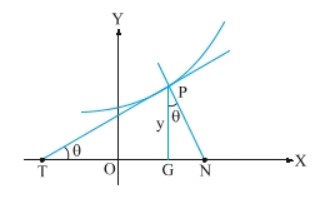
\includegraphics{images/tangentGraph}
\end{figure}
\subsubsection{Length of Subtangent}
Subtangent $= TG = \dfrac{\abs{y}}{\tan(\theta)} = \dfrac{\abs{y}}{\left( \dfrac{\dif y}{\dif x} \right)}$
\subsubsection{Length of Subnormal}
Subnormal $= GN = \abs{y} \tan(\theta) = \abs{y} \dfrac{\dif y}{\dif x}$
\subsubsection{Length of Tangent}
Tangent $= PT = \dfrac{\abs{y}}{\sin(\theta)} = \abs{y} \csc(\theta) = \abs{y} \sqrt{1 + \cot^2(\theta)} = \dfrac{\abs{y} \sqrt{1 + \left(\dfrac{\dif y}{\dif x}\right)^2}}{\abs{\dfrac{\dif y}{\dif x}}}$
\subsubsection{Length of Normal}
Normal $= PN = \abs{y} \sec(\theta) = \abs{y} \sqrt{1 + \tan^2(\theta)} = \abs{y} \sqrt{1 + \left(\dfrac{\dif y}{\dif x}\right)^2}$
\subsubsection{Length of the Curve from $a$ to $b$}
Length of curve = $\bigints\limits_a^b \left(1 + \left(\dfrac{\dif y}{\dif x}\right)^2\right) \dif x$
\subsubsection{Radius of Curvature}
$R = \dfrac{\left[ 1 + \left(\dfrac{\dif y}{\dif x}\right)^2\right]^{\dfrac32}}{\dfrac{\dif^{\;2}y}{\dif x ^2}}$
\pagebreak
\subsection{Local Maxima and Minima}
\subsubsection{Local Maximum}
\begin{define}
Let a function $f$ be defined on a set $S$. The point $c \in S$ is called a \underline{point of local maximum} if there exists an open interval $I$ containing $c$ such that $f(c) \geq f(x) \forall x \in I \cap S$ and $I$ should be a subset of $S$.
\end{define}
\subsubsection{Local Minimum}
\begin{define}
Let a function $f$ be defined on a set $S$. The point $c \in S$ is called a \underline{point of local minimum} if there exists an open interval $I$ containing $c$ such that $f(c) \leq f(x) \forall x \in I \cap S$ and $I$ should be a subset of $S$.
\end{define}
Note that Local Maxima and Local Minima don't exist at end-points because you can't have an open interval which contains the end-point and is a subset of $S$.
\subsection{Fermat's Theorem}
\begin{theorem}
If a function attains a local maximum or a local minimum at an interior point $c$, and if the function is differentiable at $c$, then $f'(c) = 0$.
\end{theorem}
\subsection{Rolle's Theorem}
\begin{theorem}
If a function $f$ is continuous in $[a, b]$ and differentiable in $(a, b)$ and $f(a) = f(b)$, then there exists at least one $c \in (a, b)$ such that $f'(c) = 0$.
\end{theorem}
\subsubsection{Conclusions}
Let $f$ be a function which is infinitely continuously differentiable (i.e. all subsequent derivatives are also continuous), then:
\begin{itemize}
\item Between two real roots of $f(x) = 0$ lies at least one real root of $f'(x) = 0$.
\item Between $n$ real roots of $f(x) = 0$ lie at least $(n - 1)$ real roots of $f'(x) = 0$
\item Between $n$ real roots of $f(x) = 0$ lie at least $(n - 2)$ real roots of $f''(x) = 0$\\
(Generalizing)
\item Between $n$ real roots of $f(x) = 0$ lie at least $(n - k)$ real roots of $f^{(k)}(x) = 0$
\item If $f^{(k)}(x) = 0$ has $(n - k)$ roots, then $f(x) = 0$ has at most $n$ roots.
\end{itemize}
\subsection{Linear Differential Equation and Inequality}
\[f'(x) + k f(x) = 0\]
\[f'(x) - k f(x) = 0\]
Whenever we see an equation or inequality of this form, we will multiply both sides by the integrating factor. The integrating factor of $f'(x) + k f(x)$ is ${\rm e}^{kx}$ and that of $f'(x) - k f(x)$ is ${\rm e}^{-kx}$. Notice that both are positive and won't change the sign of the inequality.
\begin{align*}
{\rm e}^{kx}f'(x) + k {\rm e}^{kx} f(x) = 0\\
\dfrac{\dif}{\dif x}\left({\rm e}^{kx} f(x)\right) = 0
\end{align*}
\pagebreak
\subsection{Darboux's Theorem}
\begin{theorem}
If a function $f$ is differentiable in the closed interval $I = [a, b]$ and $f'(a) < k < f'(b)$, then $\exists \; c \in (a, b) : f'(c) = k$.\\
In other words, $f'(x)$ will have intermediate value property.
\end{theorem}
\subsection{Multiplicity of Roots and Rolle's Theorem}
Suppose $f$ is a polynomial of which $\alpha$ is a zero with multiplicity $r$ where $f(x) = (x-\alpha)^r \cdot g(x)$, where $g$ is another polynomial and $g(\alpha) \neq 0$. Then $f'(x)$ has $\alpha$ as one of its zeros with multiplicity $(r - 1)$.
\begin{proof}
\begin{align*}
f(x) &= (x - \alpha)^r \cdot g(x)\\
f'(x) &= r(x - \alpha)^{r-1}\cdot g(x) + (x - \alpha)^r \cdot g'(x)\\
&= (x - \alpha)^{r-1} \left[ r g(x) + (x - \alpha) g'(x) \right]
\end{align*}
Now, observing $\left[ r g(x) + (x - \alpha) g'(x) \right]$. This won't be zero at $x = \alpha$ since $g(\alpha) \neq 0$ [given].\\
Also, $(x - \alpha)^{r-1}$ has $\alpha$ as a zero with multiplicity $(r - 1)$.\\
Therefore, $f'(x)$ will have $\alpha$ as one of its zeros with multiplicity $(r - 1)$.\\
\end{proof}
Similarly, the multiplicity of $\alpha$ in $f''(x)$ will be $(r - 2)$ and so on...\\
The converse is also true.
\pagebreak
\subsection{Problems on Rolle's Theorem and Roots}
\begin{prob}
Prove that $x {\rm e}^x = 1$ has exactly one root in $(0, 1)$.
\begin{proof}
Consider a function $f(x) = x {\rm e}^x - 1$.\\
We need to prove that $f(x)$ has at least one root in $(0, 1)$.\\
Now, $f$ is continuous everywhere, so it's also continuous in $[0, 1]$.\\
Applying Bolzano's Theorem:
\begin{align*}
f(0) &= 0 - 1 = -1 < 0\\
f(1) &= {\rm e} - 1 > 0\\
\Rightarrow f(0) \cdot f(1) &< 0
\end{align*}
Therefore, there exists \textbf{at least one} root of $f(x)$ in $(0, 1)$.\\
But we have to prove that it has exactly one root.\\
Assume for the purpose of contradiction that $f(x)$ has two roots in $(0, 1)$.\\
Then by Rolle's theorem, $f'(x)$ will have at least one root in $(0, 1)$.\\
\begin{equation*}
f'(x) = {\rm e} ^ x + x {\rm e}^x
\end{equation*}
But ${\rm e} ^ x + x {\rm e}^x > 0 \; \forall x \in (0, 1)$\\
Or, $f'(x)$ has no root in $(0, 1)$.\\ This contradicts our assumption that $f(x)$ has two roots in $(0, 1)$.\\
$\therefore f$ has exactly one root in (0, 1). 
\end{proof}
\end{prob}
\begin{prob}
Comment on the number of roots of $f(x) = x^4- 4x - 1$.\\
\textbf{Solution: } The given polynomial is of even degree and has the leading coefficient and constant term of opposite signs. Therefore it has at least 2 real roots: one in $(-\infty, 0)$ and the other in $(0, \infty)$.\\
Assume $f(x)$ has 3 or more roots.\\
Then $f'(x)$ should have at least 2 real roots.\\
\begin{align*}
f'(x) &= 4x^3 - 4\\
&= 4(x^3 - 1)
\end{align*}
But $f'(x)$ has exactly 1 real root (i.e. $x = 1$). This is a contradiction.\\
Therefore, $f(x)$ has exactly 2 roots.
\end{prob}
\pagebreak
\begin{prob}
Let $f$ be a function which is differentiable on $\mathbb{R}$ and $\alpha$ and $\beta$ be two numbers such that $\alpha < \beta$ and $f(\alpha) = f(\beta) = 0$. Then which of the following is/are correct?\\
\begin{enumerate*}[label=(\Alph*)]
\item There exists $c \in (\alpha, \beta)$ such that $f'(c) = f(c)$\\
\item There exists $c \in (\alpha, \beta)$ such that $f'(c) = 2f(c)$\\
\item There exists $c \in (\alpha, \beta)$ such that $f'(c) = 3f(c)$\\
\item There exists $c \in (\alpha, \beta)$ such that $f'(c) = kf(c)$ for any real $k$\\
\end{enumerate*}\\
\textbf{Solution: (A, B, C, D) } D is just a generalization of A, B and C. So if we prove D, that will prove all the options.\\
We have to prove that $\exists c \in (\alpha, \beta) \mid f'(c) - kf(c) = 0 \;\forall k > 0$\\
Consider $g(x) = {\rm e}^{-kx} f(x)$\\
$g$ is continuous in $[a, b]$ and differentiable in $(a, b)$\\
Now, $g(\alpha) = 0$ and $g(\beta) = 0$ because $f(\alpha) = f(\beta) = 0$ [Given]\\
Then by Rolle's Theorem,
\begin{align*}
\exists c \in (\alpha, \beta) : g'(c) &= 0\\
\Rightarrow {\rm e}^{-kc} f'(c) - k{\rm e}^{-kc}f(c) &= 0 && \text{Divide by } {\rm e}^{-kc}\\
\Rightarrow f'(c) - k f(c) &= 0\\
\Rightarrow f'(c) &= kf(c)
\end{align*}
This completes the proof. Hence all the options \textbf{A, B, C and D} are correct.
\end{prob}
\begin{prob}
If $\dfrac{a}{3} + \dfrac{b}{2} + c = 0$, then prove that the equation $ax^2 + bx + c = 0$ has at least one root in $(0, 1)$
\end{prob}
\begin{proof}
We will treat $ax^2 + bx + c$ as the derivative of some function.\\
Let $f(x) = \dfrac{ax^3}{3} + \dfrac{bx^2}{2} + cx$.
\begin{align*}
f'(x) &= ax^2 + bx + c\\
f(x) &= \dfrac{ax^3}{3} + \dfrac{bx^2}{2} + cx\\
f(1) &= \dfrac{a}3 + \dfrac{b}2 + c = 0\\
f(0) &= 0
\end{align*}
Since $f(x)$ is continuous in $[0, 1]$ and differentiable in $(0, 1)$, Applying Rolle's Theorem,\\
\begin{align*}
\Rightarrow \exists k \in (0, 1) : f'(k) &= 0\\
\Rightarrow \exists k \in (0, 1) : ak^2 + bk + c &= 0
\end{align*}
i.e. $ax^2 + bx + c = 0$ has at least one root in $(0, 1)$
\end{proof}
\pagebreak
\begin{prob}
The Legendre Polynomial is defined by the following formula (Rodrigues Formula).
\[P_n(x) = \dfrac{1}{2^n n!} \dfrac{\dif^{\;n}}{\dif x^n} (x^2 - 1)^n\]
Prove that $P_n(x)$ has $n$ different real roots, all of which are found between $-1$ and $1$.
\begin{proof}
Notice that $\dfrac{1}{2^n n!}$ is just a constant. So the roots of $P_n(x)$ will be the same as the roots of $\dfrac{\dif^{\;n}}{\dif x^n} (x^2 - 1)^n$.\\
Consider $g(x) = (x^2 - 1)^n$. This is a polynomial of degree $2n$. If we differentiate it $n$ times, we will get a polynomial of degree $n$.\\
So $\dfrac{\dif^{\;n}}{\dif x^n} (x^2 - 1)^n$ is a polynomial of degree $n$.
By the Fundamental Theorem of Algebra, it will have at most $n$ roots.\\
\begin{align*}
g(x) &=  (x^2 - 1)^n\\
&= (x+1)^n(x-1)^n
\end{align*}
$g(x)$ has two roots: $-1$ and $1$, each having multiplicity $n$.\\\\
By Rolle's Theorem, $g'(x)$ will have at least one root in $(-1, 1)$. Also $g'(x)$ will have $-1$ and $1$ as roots, each having multiplicity $(n-1)$. So $g'(x)$ has at least $3$ distinct roots.\\\\
Again applying Rolle's Theorem, between 3 roots of $g'(x)$ will lie at least 2 real roots of $g''(x)$. And $g''(x)$ will have $-1$ and $1$ as roots of multiplicity $(n-2)$. So $g''(x)$ will have at least $4$ distinct roots.\\\\
And so on...\\\\
Applying Rolle's Theorem $(n-1)$ times. Then $g^{(n-1)}(x)$ will have at least $n-1$ roots in $(0, 1)$ and also $-1$ and $1$ as roots of multiplicity $1$ each. So $g^{(n-1)}(x)$ will have at least $(n + 1)$ real roots.\\\\
\begin{figure}[h]
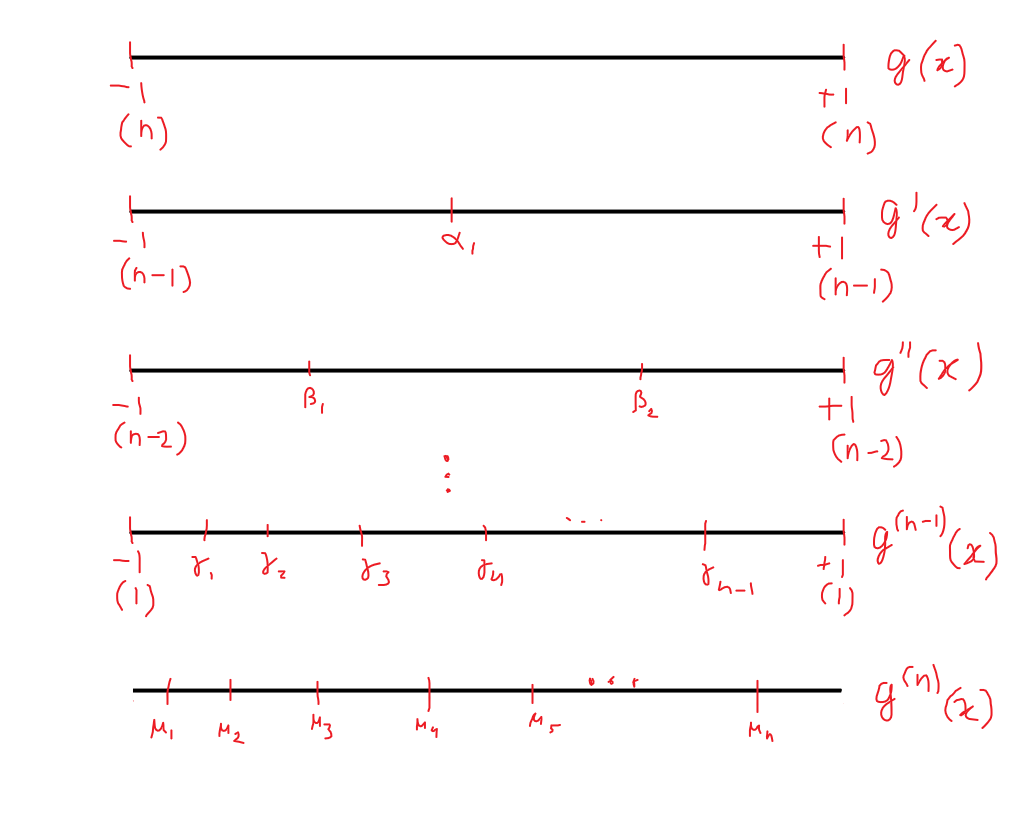
\includegraphics[scale=0.35]{images/legendre}
\end{figure}
Finally, applying Rolle's Theorem, $g^{(n)}(x)$ will have at least $n$ roots, all of which lie in $(0, 1)$.\\
Therefore, $P_n(x)$ will have exactly $n$ real roots, all of which lie in $(0, 1)$
\end{proof}
\end{prob}
\pagebreak
\subsection{Mean Value Theorems}
\subsubsection{Lagrange's Mean Value Theorem}
\begin{theorem}
If a function $f$ is continuous in $[a, b]$ and differentiable in $(a, b)$, then there exists at least one $c \in (a, b)$ such that:
\[\dfrac{f(b) - f(a)}{b - a} = f'(c)\]
Geometrically, it means at that at some point in the interval $(a, b)$, the tangent will be parallel to the chord.
\end{theorem}
\begin{proof}
Consider the following function.
\[g(x) = \left( f(b) - f(a) \right)x - f(x)\cdot (b - x)\]
Then,
\[g'(x) = f(b) - f(a) - f'(x) \cdot (b - a)\]
Now, $g$ is continuous in $[a, b]$ and differentiable in $(a, b)$ and $g(a) = g(b)$. Applying Rolle's Theorem.\\
$\exists c \in (a, b)$ such that $g'(c) = 0$.\\
\begin{align*}
\Rightarrow f(b) - f(a) - f'(c) \cdot (b - a) &= 0\\
\Rightarrow f(b) - f(a) &= f'(c) \cdot (b - a)\\
\Rightarrow \dfrac{f(b) - f(a)}{b - a} &= f'(c)
\end{align*}
\end{proof}
\subsubsection{Cauchy's Mean Value Theorem}
\begin{theorem}
Let $f$ and $g$ be two functions continuous in $[a, b]$ and differentiable in $(a, b)$, then there exists at least one $c \in (a, b)$ such that $\dfrac{f(b) - f(a)}{g(b) - g(a)} = \dfrac{f'(c)}{g'(c)}$
\end{theorem}
\begin{proof}
We need to prove that for some $x = c$, where $c \in (a, b)$, $\dfrac{f(b) - f(a)}{g(b) - g(a)} = \dfrac{f'(x)}{g'(x)}$.\\
Or $g'(x) \cdot \left( f(b) - f(a) \right) - f'(x) \cdot \left( g(b) - g(a) \right) = 0$.
Consider the following function:
\[h(x) = g(x) \cdot \left( f(b) - f(a) \right) - f(x) \cdot \left( g(b) - g(a) \right)\]
Then,
\[h'(x) = g'(x) \cdot \left( f(b) - f(a) \right) - f'(x) \cdot \left( g(b) - g(a) \right)\]
Now, $h(x)$ is  continuous in $[a, b]$ and differentiable in $(a, b)$ and $h(a) = h(b)$. Applying Rolle's Theorem.\\
$\exists c \in (a, b)$ such that $h'(c) = 0$\\
Or $g'(c) \cdot \left( f(b) - f(a) \right) - f'(c) \cdot \left( g(b) - g(a) \right) = 0$\\
$\Rightarrow \dfrac{f(b) - f(a)}{g(b) - g(a)} = \dfrac{f'(c)}{g'(c)}$\\
\end{proof}
\pagebreak
\subsubsection{Important Result from Lagrange's Mean Value Theorem}
\begin{theorem}
If $f'(x) > g'(x) \; \forall x$ and $f(a) = g(a)$, then $f(x) > g(x) \; \forall x > a$ and $f(x) < g(x) \; \forall x < a$.
\end{theorem}
\begin{proof}
Consider $h(x) = f(x) - g(x)$\\
Then $h'(x) = f'(x) - g'(x)$\\
Also, $h'(x) > 0 \; \forall x$\\
Then we have to prove that $h(x) > 0 \; \forall x > a$ and $h(x) < 0 \; \forall x < a$.\\
Now,
\begin{align*}
h(a) = f(a) - g(a) = 0 && \because f(a) = g(a) \text{ [given]}
\end{align*}
Consider any real number $x \neq a$.\\
Note that $h$ is continuous and differentiable. Applying Lagrange's Mean Value Theorem.
\[\exists c : \dfrac{h(x) - h(a)}{x - a} = h'(c) > 0\]
\textbf{Case 1:} $x > a$\\
Then $x - a > 0$,\\
Therefore,\\
\[h(x) - h(a) > 0\]
\[\Rightarrow h(x) > h(a)\]
\textbf{Case 2:} $x < a$\\
Then $x - a < 0$,\\
Therefore,\\
\[h(x) - h(a) < 0\]
\[\Rightarrow h(x) < h(a)\]
\end{proof}
\pagebreak
\subsubsection{Example Problems}
\begin{prob}
Suppose $f'(x) \geq M$ in the interval $[a, b]$, then prove that $f(b) \geq f(a) + M(b - a)$
\end{prob}
\begin{proof}
$f(x)$ is continuous in $[a, b]$ and differentiable in $(a, b)$.\\
Applying Lagrange's Mean Value Theorem.
\[\exists c \in (a, b) : \dfrac{f(b) - f(a)}{b - a} = f'(c)\]
But $f'(x) \geq M \; \forall x \in [a, b]$ (Given), so\\
\begin{align*}
\dfrac{f(b) - f(a)}{b - a} &\geq M\\
f(b) - f(a) &\geq M (b - a)\\
f(b) &\geq f(a) + M (b - a)
\end{align*}
\end{proof}
\begin{prob}
Suppose $f'(x) \leq M$ in the interval $[a, b]$, then prove that $f(b) \leq f(a) + M(b - a)$
\end{prob}
\begin{proof}
$f(x)$ is continuous in $[a, b]$ and differentiable in $(a, b)$.\\
Applying Lagrange's Mean Value Theorem.
\[\exists c \in (a, b) : \dfrac{f(b) - f(a)}{b - a} = f'(c)\]
But $f'(x) \leq M \; \forall x \in [a, b]$ (Given), so\\
\begin{align*}
\dfrac{f(b) - f(a)}{b - a} &\leq M\\
f(b) - f(a) &\leq M (b - a)\\
f(b) &\leq f(a) + M (b - a)
\end{align*}
\end{proof}
\begin{prob}
Let the second derivative $f''$ of a function be continuous and satisfy $\abs{f''(x)} \leq 1$. If $f(0) = f(1)$, show that $\abs{f'(x)} < 1 \;\forall x \in (0, 1)$.
\end{prob}
\begin{proof} $\text{}$\\
$f$ is continuous in $[0, 1]$ and differentiable in $(0, 1)$, and $f(0) = f(1)$. Applying Rolle's Theorem.\\
$\exists c \in (0, 1) : f'(c) = 0$ or $\abs{f'(c)} \leq 1$\\
But we have to prove it for all $x$ not just some specific value.\\
\textbf{General advice:} If you see an inequality in the second derivative, using Lagrange's Mean Value Theorem could be helpful.\\
Applying Lagrange's Mean Value Theorem.\\
Consider any $x \in (0, 1) - \{c\}$.\\
The function $f'$ is continuous in $[x, c]$ or $[c, x]$ and differentiable in $(x, c)$ or $(c, x)$
\[\dfrac{f'(x) - f'(c)}{x - c} = f''(c_1) \text{\; for some } c_1 \in (x, c) \text{ or } (c, x)\]
\[\abs{f'(x) - f'(c)} = \abs{x - c} \cdot \abs{f''(c_1)} \;\; [\text{Now, } f'(c) = 0 \text{ and } \abs{f''(c_1)} \leq 1 ]\]
\[\abs{f'(x)} = \abs{x - c} \cdot \abs{f''(c_1)} \leq \abs{x - c} < 1\]
\end{proof}
\pagebreak
\begin{prob}
Assume that $\abs{f''(x)} \leq m$ for each $x$ in the interval $[0, a]$ and assume that $f$ takes its largest value at an interior point in this interval. If $f''$ is continuous in the closed interval $[0, a]$, show that $\abs{f'(0)} + \abs{f'(a)}\leq am$ where $f'(0)$ denotes the right-hand derivative of $f$ at $0$ and $f'(a)$ denotes the left-hand derivative of $f$ at $a$.
\end{prob}
\begin{proof}
$f$ takes its largest value at an interior point of $[0, a]$.\\
Or, $f$ has a point of maximum in $(0, a)a$.\\
By Fermat's Theorem, \[\exists c \in (0, a) : f'(c) = 0\]\\
Applying Lagrange's Mean Value Theorem on $f'$ in $[0, c]$.\\
\[\dfrac{f'(0) - f'(c)}{0 - c} = f''(c_1) \text{\;\;\; for some } c_1 \in (0, c)\]
But $f'(c) = 0$\\
Taking modulus on both sides and multiplying by $\abs{c}$
\[\abs{f'(0)} = \abs{c} \cdot \abs{f''(c_1)}\]
But $\abs{f''(c_1)}\leq m$
\begin{equation}\label{eqn:c1}
\abs{f'(0)} = \abs{c} \cdot \abs{f''(c_1)} \leq \abs{c} \cdot m
\end{equation}
Applying Lagrange's Mean Value Theorem on $f'$ in $[c, a]$.\\
\[\dfrac{f'(a) - f'(c)}{a - c} = f''(c_2) \text{\;\;\; for some } c_2 \in (c, a)\]
But $f'(c) = 0$
Taking modulus on both sides and multiplying by $\abs{a - c}$
\[\abs{f'(a)} = \abs{a - c} \cdot \abs{f''(c_2)}\]
But $\abs{f''(c_2)} \leq m$
\begin{equation}\label{eqn:c2}
\abs{f'(a)} = \abs{a - c} \cdot \abs{f''(c_2)} \leq \abs{a - c} \cdot m
\end{equation}
Adding $(\ref{eqn:c1})$ and $(\ref{eqn:c2})$,
\begin{align*}
\abs{f'(0)} + \abs{f'(a)} &\leq \abs{c} \cdot m + \abs{a - c} \cdot m\\
\abs{f'(0)} + \abs{f'(a)} &\leq m \cdot \left(\abs{c} + \abs{a - c}\right)\\
\abs{f'(0)} + \abs{f'(a)} &\leq m \cdot \abs{a} && \text{But } a \geq 0 \text{ so } \abs{a} = a \\
\Rightarrow \abs{f'(0)} + \abs{f'(a)} &\leq a m
\end{align*}
\end{proof}
\pagebreak
\begin{prob}
Suppose $f$ is continuous on $[a, b]$ and differentiable on $(a, b)$. Assume further that $f(b) - f(a) = b - a$, then prove that for all positive integer $n$, there exist distinct points $c_1, c_2, c_3, \cdots, c_n$ such that $f'(c_1) + f'(c_2) + f'(c_3) + \cdots + f'(c_n) = n$.
\end{prob}
\begin{proof}
We will try to prove it for $n = 1$ and $n = 2$, and then we'll try to draw inspiration from it to prove for any general $n$.\\
\textbf{For $n = 1$,}\\
$f$ is continuous in $[a, b]$ and differentiable in $(a, b)$.\\
Applying Lagrange's Mean Value Theorem.\\
\[
\exists c_1 \in (a, b) : \dfrac{f(b) - f(a)}{b - a} = f'(c_1)
\]
But $f(b) - f(a) = b - a$ (Given),
\begin{align*}
\Rightarrow\exists c_1 \in (a, b) &: \dfrac{\cancel{b - a}}{\cancel{b - a}} = f'(c_1)\\
\Rightarrow\exists c_1 \in (a, b) &: f'(c_1) = 1
\end{align*}
And this proves the result for $n = 1$.\\
\textbf{For $n = 2$,}\\
We need to prove that there exist $c_1$ and $c_2$ such that $f'(c_1) + f'(c_2) = 2$
We will divide the interval $[a, b]$ into $2$ equal parts using the point $\dfrac{a + b}{2}$.\\
Applying Lagrange's Mean Value Theorem and Adding the equations.\\
For some $c_1$ and $c_2$,
\begin{align*}
\cancel{f\left(\dfrac{a+b}{2}\right)} - f(a) &= \dfrac{b-a}{2} f'(c_1)\\
f(b) - \cancel{f\left(\dfrac{a+b}{2}\right)} &= \dfrac{b - a }{2} f'(c_2)\\
\cline{0-1}
f(b) - f(a) &= \dfrac{b - a}{2} \left(f'(c_1) + f'(c_2)\right)\\
\cline{0-1}
\end{align*}
$\Rightarrow \dfrac{f(b) - f(a)}{b - a} = \dfrac12 \left(f'(c_1) + f'(c_2)\right)$\\
But $f(b) - f(a) = b - a$ (Given),
\[\Rightarrow \dfrac{\cancel{b - a}}{\cancel{b - a}} = \dfrac12 \left(f'(c_1) + f'(c_2)\right) \]
\[f'(c_1) + f'(c_2) = 2\]
This proves the result for $n = 2$.
\pagebreak
Now we will prove it for any general $n$ by the same analogy.\\\\
\textbf{For any General $n$,}\\
For the case of $n = 2$, we divided the interval $(a, b)$ into two equal parts.\\
So for the general case, we will try to divide the interval into $n$ equal parts, i.e. $\left(a, a + \dfrac{b - a}{n}\right),\\ \left(a + \dfrac{b - a}{n}, a + \dfrac{2(b - a)}{n}\right), \left(a + \dfrac{2(b - a)}{n}, a + \dfrac{3(b - a)}{n}\right), \cdots, \left(a + \dfrac{(n-1)(b - a)}{n}, b\right)$\\\\
Applying Lagrange's Mean Value Theorem $n$ times (on each of these intervals) and adding all the resulting equations. This makes a telescopic sum. There exist $c_1, c_2, c_3, \cdots, c_n$ such that:
\begin{align*}
\cancel{f\left(a + \dfrac{b - a}{n}\right)} - f(a) &= \left(\dfrac{b - a}{n}\right) \cdot f'(c_1)\\
\cancel{f\left(a + \dfrac{2(b - a)}{n}\right)} - \cancel{f\left(a + \dfrac{b - a}{n}\right)} &= \left(\dfrac{b - a}{n}\right) \cdot f'(c_2)\\
\cancel{f\left(a + \dfrac{3(b - a)}{n}\right)} - \cancel{f\left(a + \dfrac{2(b - a)}{n}\right)} &= \left(\dfrac{b - a}{n}\right) \cdot f'(c_3)\\
\cancel{f\left(a + \dfrac{3(b - a)}{n}\right)} - \cancel{f\left(a + \dfrac{2(b - a)}{n}\right)} &= \left(\dfrac{b - a}{n}\right) \cdot f'(c_3)\\
\cancel{f\left(a + \dfrac{4(b - a)}{n}\right)} - \cancel{f\left(a + \dfrac{3(b - a)}{n}\right)} &= \left(\dfrac{b - a}{n}\right) \cdot f'(c_4)\\
\vdots\;\;\;\;\;\;\;\;\;\;\;\;\;\;\;\;\;\;\;\;\;\;\;\;\vdots\;\;\;\;\;\;\;\;\;\;\;\;\;&= \;\;\;\;\;\;\;\;\vdots\\
f\left(b \right) - \cancel{f\left(a + \dfrac{(n-1)(b - a)}{n}\right)} &= \left(\dfrac{b - a}{n}\right) \cdot f'(c_n)\\
\cline{0-1}
f(b) - f(a) &= \left(\dfrac{b-a}{n}\right)\cdot \left(f'(c_1) + f'(c_2) + \cdots + f'(c_n)\right)\\
\cline{0-1}
\end{align*}
$\Rightarrow \dfrac{f(b) - f(a)}{b - a} =\dfrac1{n} \left(f'(c_1) + f'(c_2) + \cdots + f'(c_n)\right)$\\\\
But $f(b) - f(a) = b - a$
\begin{align*}
\Rightarrow \dfrac{\cancel{b - a}}{\cancel{b - a}} =\dfrac1{n} \left(f'(c_1) + f'(c_2) + \cdots + f'(c_n)\right)\\
\Rightarrow f'(c_1) + f'(c_2) + f'(c_3) + \cdots + f'(c_n) = n
\end{align*}
\end{proof}
\pagebreak
\subsubsection*{Proving Some Inequalities}
\begin{prob}
Prove that $\forall a, b \in \mathbb{R}$, 
\[\abs{\sin(a) - \sin(b)} \leq \abs{a - b}\]
\end{prob}
\begin{proof} (using Lagrange's Mean Value Theorem)\\
\textbf{Case 1:} If $a = b$\\
This inequality is trivially true if $a = b$, because $LHS = \sin(a) - \sin(a) = 0$ and $RHS = a - a = 0$\\\\
\textbf{Case 2:} If $a \neq b$\\
Consider a function $f(x) = \sin(x)$
$f$ is continuous and differentiable everywhere. Applying Lagrange's Mean Value Theorem.\\
There exists $c \in (a, b)$ or $(b, a)$ such that
\begin{align*}
\dfrac{\sin(a) - \sin(b)}{a - b} &= \cos(c)\\
\Rightarrow \abs{\dfrac{\sin(a) - \sin(b)}{a - b}} &= \abs{\cos(c)} \leq 1 && \text{Multiply by } \abs{a - b}\\
\Rightarrow \abs{\sin(a) - \sin(b)} &\leq \abs{a - b}
\end{align*}
\end{proof}
\begin{prob}
Prove that $\forall x > 0$,
\[\dfrac{x}{1+x} < \log_{\rm e}(1+x) < x\]
\end{prob}
\begin{proof}
Consider the function $f(t) = \log_{\rm e}(t)$\\
$f$ is continuous in $[1, 1+x]$ and differentiable in $(1, 1+x)$. Applying Lagrange's Mean Value Theorem.\\
There exists $c \in (1, 1 + x)$ such that
\[\dfrac{\ln(1 + x) - \ln(1)}{1 + x - 1} = \dfrac1{c}\]
Now,
\[1 < c < 1+x\]
\[\Rightarrow \dfrac1{1 + x} < \dfrac1{c} < 1\]
\[\Rightarrow \dfrac1{1 + x} < \dfrac{\ln(1 + x) - \ln(1)}{\cancel{1} + x \cancel{- 1}} < 1\]
But $\ln(1) = 0$
\[\Rightarrow \dfrac1{1 + x} < \dfrac{\ln(1 + x)}{x} < 1\]
Now, $x > 0$ (Given), so multiplying by x,
\[\dfrac{x}{1 + x} < \ln(1+x) < x\]
\end{proof}
\pagebreak
\begin{prob}
Show that the square roots two successive natural numbers greater than $N^2$ differ by less than $\dfrac1{2N}$.
\end{prob}
\begin{proof}
Consider any two consecutive natural numbers $m$ and $m + 1$, both greater than $N^2$.\\
Also consider the function $f(x) = \sqrt{x}$.\\
Applying Lagrange's Mean Value Theorem,\\
$f(x)$ is continuous in $[m, m + 1]$ and differentiable in $(m, m + 1)$.\\
Therefore, there exists $c \in (m, m+1)$ such that
\begin{align*}
\dfrac{\sqrt{m + 1} - \sqrt{m}}{m + 1 - m} &= f'(c)\\
\sqrt{m + 1} - \sqrt{m} &= \dfrac{1}{2\sqrt{c}}
\end{align*}
Now,
\[m < c < m + 1\]
\[\sqrt{m} < \sqrt{c} < \sqrt{m + 1}\]
\[\dfrac1{\sqrt{m + 1}} < \dfrac{1}{\sqrt{c}} < \dfrac1{\sqrt{m}}\]
Also, it is given that
\[N^2 < m < m + 1\]
\[\Rightarrow N < \sqrt{m} < \sqrt{m + 1}\]
\[\Rightarrow\dfrac1{\sqrt{m + 1}} < \dfrac1{\sqrt{m}} < \dfrac{1}{N}\]
So $\dfrac1{\sqrt{c}} < \dfrac1{\sqrt{m}}$ and $\dfrac{1}{\sqrt{m}} < \dfrac1{N}$
\[\Rightarrow \dfrac1{\sqrt{c}} < \dfrac1{N}\]
Therefore,
\[\sqrt{m + 1} - \sqrt{m} = \dfrac{1}{2\sqrt{c}} < \dfrac{1}{2N}\]
\[\Rightarrow\sqrt{m + 1} - \sqrt{m} < \dfrac{1}{2N}\]
\end{proof}
\begin{prob}
If $f$ and $g$ are differentiable functions in $(0, 1)$ satisfying $f(0) = 2 = g(1)$, $g(0) = 0$ and $f(1) = 6$, then for some $c \in [0, 1]$:\\\\
\begin{enumerate*}[label=(\Alph*)]
\item $2 f'(c) = g'(c)$\\
\item $2 f'(c) = 3g'(c)$\\
\item $f'(c) = g'(c)$\\
\item $f'(c) = 2 g'(c)$
\end{enumerate*}
\end{prob}
\paragraph{Solution: (D)}
Simply invoke Cauchy's Mean Value Theorem.\\
\[\exists c \in (0, 1) : \dfrac{f(1) - f(0)}{g(1) - g(0)} = \dfrac{f'(c)}{g'(c)}\]
\[\Rightarrow \dfrac{f'(c)}{g'(c)} = \dfrac{6 - 2}{2-0} = 2 \Rightarrow f'(c) = 2 g'(c)\]
\pagebreak
\subsubsection{Differentiation of Determinants}
To differentiate a determinant, we differentiate each row (or column) one at a time, leaving the rest unchanged, and take the sum.
\[\text{Let } p(x)= 
\begin{vmatrix}a(x)&b(x)&c(x)\\d(x)&e(x)&f(x)\\g(x)&h(x)&i(x)\end{vmatrix}
\]
Then
\[p'(x) = 
\begin{vmatrix}a'(x)&b'(x)&c'(x)\\d(x)&e(x)&f(x)\\g(x)&h(x)&i(x)\end{vmatrix} +
\begin{vmatrix}a(x)&b(x)&c(x)\\d'(x)&e'(x)&f'(x)\\g(x)&h(x)&i(x)\end{vmatrix} +
\begin{vmatrix}a(x)&b(x)&c(x)\\d(x)&e(x)&f(x)\\g'(x)&h'(x)&i'(x)\end{vmatrix}
\]
Or
\[p'(x) = 
\begin{vmatrix}a'(x)&b(x)&c(x)\\d'(x)&e(x)&f(x)\\g'(x)&h(x)&i(x)\end{vmatrix} +
\begin{vmatrix}a(x)&b'(x)&c(x)\\d(x)&e'(x)&f(x)\\g(x)&h'(x)&i(x)\end{vmatrix} +
\begin{vmatrix}a(x)&b(x)&c'(x)\\d(x)&e(x)&f'(x)\\g(x)&h(x)&i'(x)\end{vmatrix}
\]
\subsubsection{The General Mean Value Theorem}
\begin{theorem}
Let $f$, $g$ and $h$ be functions which are continuous in $[a, b]$ and differentiable in $(a, b)$, then there exists at least one $c \in (a, b)$ such that
\[
\begin{vmatrix}
f'(c) & g'(c) & h'(c)\\
f(a) & g(a) & h(a)\\
f(b) & g(b) & h(b)
\end{vmatrix} = 0
\]
\end{theorem}
\begin{proof}
Consider the function $p$ defined as the following.
\[p(x) = 
\begin{vmatrix}
f(x) & g(x) & h(x)\\
f(a) & g(a) & h(a)\\
f(b) & g(b) & h(b)
\end{vmatrix}
\]
Then,
\begin{align*}
p'(x) &= 
\begin{vmatrix}
f'(x) & g'(x) & h'(x)\\
f(a) & g(a) & h(a)\\
f(b) & g(b) & h(b)
\end{vmatrix}
+
\begin{vmatrix}
f(x) & g(x) & h(x)\\
0 & 0 & 0\\
f(b) & g(b) & h(b)
\end{vmatrix}
+
\begin{vmatrix}
f(x) & g(x) & h(x)\\
f(a) & g(a) & h(a)\\
0 & 0 & 0
\end{vmatrix}\\
&=
\begin{vmatrix}
f'(x) & g'(x) & h'(x)\\
f(a) & g(a) & h(a)\\
f(b) & g(b) & h(b)
\end{vmatrix}
\end{align*}
Now, $p$ is continuous in $[a, b]$ and differentiable in $(a, b)$ because $f$, $g$ and $h$ are continuous in $[a, b]$ and differentiable in $(a, b)$.\\
Also, $p(a) = 0$ (because that would make the first two rows equal) and similarly $p(b) = 0$.\\
Applying Rolle's Theorem on $p$,
\[\exists c \in (a, b) : p'(c) = 0\]
\[\exists c \in (a, b) :
\begin{vmatrix}
f'(c) & g'(c) & h'(c)\\
f(a) & g(a) & h(a)\\
f(b) & g(b) & h(b)
\end{vmatrix} = 0
 \]
\end{proof}
\pagebreak
\subsection{Monotonicity}
\subsubsection{Definitions}
\begin{define}
A function $f$ is said to be \underline{non-decreasing} or \underline{monotonically increasing} in an interval if for all $x_1, x_2$ in the interval, $x_1 > x_2 \Rightarrow f(x_1) \geq f(x_2)$
\end{define}
\begin{define}
A function $f$ is said to be \underline{non-increasing} or \underline{monotonically decreasing} in an interval if for all $x_1, x_2$ in the interval, $x_1 > x_2 \Rightarrow f(x_1) \leq f(x_2)$
\end{define}
\begin{define}
A function $f$ is said to be \underline{strictly increasing} in an interval if for all $x_1, x_2$ in the interval, $x_1 > x_2 \Rightarrow f(x_1) > f(x_2)$
\end{define}
\begin{define}
A function $f$ is said to be \underline{strictly decreasing} in an interval if for all $x_1, x_2$ in the interval, $x_1 > x_2 \Rightarrow (x_1) < f(x_2)$
\end{define}\;\\
Note that by these definitions, the constant function is both monotonically increasing and monotonically decreasing.\\
Also note that a function doesn't have to be continuous or differentiable in order for it to be increasing or decreasing.
\subsubsection{Properties}
\begin{enumerate}
\item If a function is increasing in an interval $[a, b]$, then for this interval, the function assumes its greatest value at $b$ and its least value at $a$.
\item Similarly, if a function is decreasing in an interval $[a, b]$, then for this interval, the function assumes its greatest value at $a$ and its least value at $b$.
\item Let $f$ be a function which is continuous in $[a, b]$ and differentiable in $(a, b)$. Then,
\begin{enumerate}
\item If $f'(x) \geq 0 \; \forall x \in (a, b)$, then the function is monotonically increasing (or non-decreasing) in the interval.
\item If $f'(x) \leq 0 \; \forall x \in (a, b)$, then the function is monotonically decreasing (or non-increasing) in the interval.
\item If $f'(x) > 0 \; \forall x \in (a, b)$, then the function is strictly increasing in the interval.
\item If $f'(x) < 0 \; \forall x \in (a, b)$, then the function is strictly decreasing in the interval.
\end{enumerate}
\item A function can have its derivative equal to zero somewhere and still be strictly increasing or decreasing (For example, $y=x^3$ is strictly increasing). Let $f$ be a function continuous in $[a, b]$ and differentiable in $(a, b)$. Then,
\begin{enumerate}
\item If $f'(x) \geq 0 \; \forall x \in (a, b)$ and the equality holds at discrete points, then the function is strictly increasing.
\item If $f'(x) \leq 0 \; \forall x \in (a, b)$ and the equality holds at discrete points, then the function is strictly decreasing.
\end{enumerate}
\item Let $f$ be a continuous and differentiable function.\\ Then, $f$ is strictly increasing or strictly decreasing $\Leftrightarrow$ $f$ is one-one.
\pagebreak
\item If $f$ is increasing and $g$ is increasing, then $f\circ g$ is increasing.
\begin{proof}
Consider any two real numbers $a$ and $b$ such that $a < b$.\\
$\Rightarrow g(a) < g(b)$ because $g$ is increasing.\\
$\Rightarrow f(g(a)) < f(g(b))$ because $f$ is increasing.\\
$\Rightarrow (f \circ g)$ is decreasing
\end{proof}
\item Similarly if $f$ is decreasing and $g$ is decreasing, then $f \circ g$ is increasing.
\end{enumerate}
\subsubsection{Problems}
\begin{prob}
Find the total number of positive integer solutions of $a^b = b^a$ (where $b>a$).
\end{prob}
\paragraph{Solution:}
\begin{align*}
a^b &= b^a && \text{Raise both sides to } \dfrac1{ab}^{th}\text{ power}\\
\Rightarrow a^{\left(\dfrac{1}{a}\right)} &= b^{\left(\dfrac{1}{a}\right)} && \text{Take natural log  on both sides}\\
\Rightarrow \dfrac{1}{a} \ln(a) &= \dfrac{1}{b} \ln(b)\\
\Rightarrow \dfrac{\ln(a)}{a} &= \dfrac{\ln(b)}{b}\\
\Rightarrow \dfrac{a}{\ln(a)} &= \dfrac{b}{\ln(b)}
\end{align*}
Consider the function $f(x) = \dfrac{x}{\ln(x)}$, $x > 0$\\
Then we're looking for solutions of $f(a) = f(b)$ where $a, b \in \mathbb{Z}^+$, $b > a$.
\begin{align*}
f(x) &= \dfrac{x}{\ln(x)}\\\\
\Rightarrow f'(x) &= \dfrac{\ln(x) - 1}{(\ln(x))^2}
\end{align*}
Now, $f'(x) = 0$ at $x = {\rm e}$\\
So $f(x) > 0$ for $x \in ( {\rm e}, \infty)$ and $f(x) < 0$ for $x \in (0, {\rm e})$\\
Therefore $f$ is strictly decreasing in $(0, {\rm e})$ and $f$ is strictly increasing in $({\rm e}, \infty)$\\
$\Rightarrow f$ is one-one in $(0, {\rm e})$ and one-one in $({\rm e}, \infty)$\\
In other words, $f(a) = f(b)$ has no solution for $a, b \in (0, {\rm e})$ and $a, b \in ({\rm e}, \infty)$\\
Then the only case that remains is when $a \in (0, {\rm e})$ and $b \in ({\rm e}, \infty)$.\\
There are only two positive integers in $(0, e)$, namely 1 and 2.\\
If $a = 1$, we get
\[1^b = b ^1\]
where $b > 1$.\\
LHS = 1 but RHS will always be greater than $1$.\\
So there will be no solution corresponding to $a = 1$
Now, if $a = 2$, we get
\[2^b = b^2\]
There exists exactly one integer solution to this, i.e. $a = 2$ and $b = 4$.
\[2^4 = 4^2\]
Therefore, $a^b = b^a$ will have exactly one positive-integer solution for $b > a$.
\pagebreak
\begin{prob}
Let $\alpha$ be a repeated root of a quadratic equation $f(x) = 0$ and $A(x), B(x)$ and $C(x)$ be polynomials of degree 3, 4 and 5 respectively. Then show that $\begin{vmatrix}
A(x)&B(x)&C(x)\\A(\alpha)&B(\alpha)&C(\alpha)\\A'(\alpha)&B'(\alpha)&C'(\alpha)
\end{vmatrix}$ is divisible by $f(x)$.
\end{prob}
\begin{proof}
$\alpha$ is a root of $f(x)$. 
\[
f(\alpha) = 0
\]
\[
\Rightarrow f(x) = a(x - \alpha)^2
\]
Also, since $\alpha$ is a repeated root of $f(x)$, this implies $\alpha$ is also a root of $f'(x)$.
\[f'(\alpha) = 0\]
Now
\[\text{Let } h(x) = \begin{vmatrix}
A(x)&B(x)&C(x)\\A(\alpha)&B(\alpha)&C(\alpha)\\A'(\alpha)&B'(\alpha)&C'(\alpha)
\end{vmatrix}\]
\[h(\alpha) = 0\]
\[h'(x) = \begin{vmatrix}
A'(x)&B'(x)&C'(x)\\A(\alpha)&B(\alpha)&C(\alpha)\\A'(\alpha)&B'(\alpha)&C'(\alpha)
\end{vmatrix} + 0 + 0 = \begin{vmatrix}
A'(x)&B'(x)&C'(x)\\A(\alpha)&B(\alpha)&C(\alpha)\\A'(\alpha)&B'(\alpha)&C'(\alpha)
\end{vmatrix}\]
Therefore,
\[h'(\alpha) = 0\]
$\Rightarrow \alpha$ has a multiplicity of $2$ in $h(x)$.\\
$\Rightarrow h(x)$ is divisible by f(x).\\
\end{proof}
\begin{prob}
Let $p(x)$ be a polynomial such that $p(1) = 0$ and $\dfrac{\dif}{\dif x} p(x) > p(x) \; \forall x > 1$. Show that $p(x) > 0 \; \forall x > 1$. 
\end{prob}
\begin{proof}
\begin{align*}
\dfrac{\dif}{\dif x} \left(p(x)\right) &> p(x) && \forall x > 1\\
\Rightarrow p'(x) &> p(x) && \forall x > 1\\
\Rightarrow p'(x) - p(x) &> 0 && \forall x > 1\\
\text{Multiply by the integrating factor } {\rm e}^{-x}\\
\Rightarrow {\rm e}^{-x} p'(x) - {\rm e}^{-x} p(x) &> 0 && \forall x > 1\\
\Rightarrow \dfrac{\dif}{\dif x} \left( {\rm e}^{-x} \cdot p(x) \right) &>0 && \forall x > 1
\end{align*}
Let $g(x) = {\rm e}^{-x}\cdot p(x)$.\\
Then, $g'(x) > 0 \; \forall x > 1 \Rightarrow g$ is strictly increasing $\forall x > 1$\\
And $g(1) = {\rm e}^{-1} p(1) = 0$\\
$\Rightarrow g(x) > 0 \; \forall x > 1$\\
$\Rightarrow {\rm e}^{-x} \cdot p(x) > 0$\\ 
$\Rightarrow p(x) > 0 \; \forall x > 1$
\end{proof}
\textbf{Actually, this problem is fundamentally flawed.} We can prove that no such polynomial exists by contradiction. However, such a function can exist. Had $p(x)$ been given as a differentiable function, this problem and solution would have been valid.
\pagebreak
\paragraph{Proof that such a polynomial doesn't exist:}
\begin{proof} (By contradiction)\\
Assume for the purpose of contradiction that such a polynomial exists. Let us call it $p(x).$\\
\[p(x) = a_n x^n + a_{n-1} x^{n-1} + a_{n-2} x^{n-2} + \cdots + a_3 x^3 + a_2 x^2 + a_1 x + a_0\]
\[\Rightarrow p'(x) = n a_n x^{n-1} + (n-1)a_{n-1}x^{n-2} + (n-2) a_{n-2}x^{n-3} + \cdots + a_1\]
Now, it is given that $p'(x) > p(x) \forall x > 1$\\
i.e. $p'(x) - p(x) > 0\; \forall x > 1$
\begin{align*}
p'(x) - p(x) &= -a_n x^n + x^{n-1} (na_n - a_{n-1}) + x^{n-2} \left((n-1)a_{n-1} - a_{n-2}\right)+ \cdots \\
&= -a_n x^n - x^{n-1}(a_{n-1} - na_n) - x^{n-2} \left( a_{n-2} - (n-1)a_{n-1}\right) - \cdots
\end{align*}
If $p'(x) - p(x) > 0 \; \forall x > 1$
\[-a_n x^n - x^{n-1}(a_{n-1} - na_n) - x^{n-2} \left( a_{n-2} - (n-1)a_{n-1}\right) - \cdots > 0 \; \forall x > 1\]
Then this should also be true for values of $x$ approaching infinity.\\
\[\Rightarrow a_n < 0\]
But we proved that $p(x) > 0 \; \forall x > 1$.
\[\Rightarrow a_n x^n + a_{n-1} x^{n-1} + a_{n-2} x^{n-2} + \cdots + a_3 x^3 + a_2 x^2 + a_1 x + a_0 > 0 \;\forall x > 1\]
This should also be true for infinitely great values of x.
\[\Rightarrow a_n > 0\]
And we have derived a contradiction.\\
Therefore the assumption that such a polynomial exists is incorrect.\\
Hence, the given problem is fundamentally flawed.
\end{proof}
\pagebreak
\begin{prob}
If $f : \mathbb{R} \to \mathbb{R}$ is a differentiable function such that $f'(x) > 2f(x) \; \forall x \in \mathbb{R}$ and $f(0) = 1$. Then:\\
\begin{enumerate*}[label=(\Alph*)]
\item $f(x) > {\rm e}^{2x}$ in $(0, \infty)$\\
\item $f(x)$ is decreasing in $(0, \infty)$\\
\item $f(x)$ is increasing in $(0, \infty)$\\
\item $f'(x) < {\rm e}^{2x}$ in $(0, \infty)$\\
\end{enumerate*}
\textbf{Solution: (AC)}\\
\begin{align*}
f'(x) &> 2f(x) && \text{(Given)}\\
\Rightarrow f'(x) - 2f(x) &> 0 && \text{(Multiply by the integrating factor)}\\ 
\Rightarrow {\rm e}^{-2x} f'(x) - 2 {\rm e}^{-2x} f(x) &> 0\\
\Rightarrow \dfrac{\dif}{\dif x}\left( {\rm e}^{-2x} f(x) \right) &> 0 && \text{Let } g(x) = {\rm e}^{-2x} f(x)\\
\Rightarrow g'(x) &> 0 && \forall x \in \mathbb{R}\\
\Rightarrow g(x) \text{ is strictly increasing.}\\
\Rightarrow g(x) &> g(0) && \forall x > 0\\
\Rightarrow g(x) &> {\rm e}^0 f(0) && \forall x > 0\\
\Rightarrow {\rm e}^{-2x} f(x) &> 1 && \forall x > 0\\
\Rightarrow f(x) &> {\rm e}^{2x} && \forall x \in (0, \infty)\\
\text{Therefore, option A is correct}\\
\text{Now, since } f'(x) > 2f(x) \text{ and } f(x) > {\rm e}^{2x},\\
\Rightarrow f'(x) > 2f(x) &> 2 {\rm e}^{2x} && \forall x \in (0, \infty)\\
\Rightarrow f'(x) &> 2{\rm e}^{2x} && \forall x \in (0, \infty)\\
\Rightarrow f'(x) &> 0 && \forall x \in (0, \infty)\\ 
\Rightarrow f(x) \text{ is strictly increasing in } (0, \infty)\\
\text{Therefore, option C is correct}
\end{align*}
\end{prob}
\pagebreak
\subsection{Testing for Local Maxima and Minima}
\begin{define}
The critical point of a function is defined as a point where the derivative of the function is either zero or not defined.
\end{define}
\begin{algo}
Consider a function $f(x)$. We have to find its local maxima and minima.
\begin{enumerate}
\item Differentiate $f$ to get $f'(x)$.
\item Find all the points where $f'(x)$ changes sign.
\item If $f'(x)$ changes sign from positive to negative, then the point is a local maximum. If $f'(x)$ changes sign from negative to positive, then the point is a local minimum.
\end{enumerate}
This algorithm is preferred as it gives the answer definitively and in exactly 3 steps.
\end{algo}
\begin{prob}
The function $f(x) = x\left(x^2 - 4\right)^n\left(x^2 - x + 1\right)$, $n \in \mathbb{N}$ assumes a local minimum at $x = 2$, then:\\
\begin{enumerate*}[label=(\Alph*)]
\item $n$ can be any odd number\\
\item $n$ can only be an odd prime number\\
\item $n$ can be any even integer\\
\item $n$ can only be a multiple of four\\
\end{enumerate*}
\paragraph{Solution: (C)}
\[f(x) = x\left(x^2 - 4\right)^n\left(x^2 - x + 1\right)\]
\begin{align*}
f'(x) &= (x^2 - 4)^n \cdot (x^2 - x + 1) + n(x^2-4)^{n-1} \cdot(2x)(x)(x^2-x+1) + x(x^2-4)^n \cdot (2x-1)\\
&= (x^2 - 4)^{n-1}\left( (x^2-4)(x^2-x+1) + n(2x)(x)(x^2-x+1)+x(x^2-4)(2x-1) \right)
\end{align*}
By Fermat's Theorem, since $f$ attains a local maximum at $x = 2$,
\[f'(2) = 0\]
\[\Rightarrow n - 1 \geq 1\]
\[\Rightarrow n \geq 2\]
Now, \\
$\left( (x^2-4)(x^2-x+1) + n(2x)(x)(x^2-x+1)+x(x^2-4)(2x-1) \right)$ is positive in the neighbourhood of $x=2$.\\
So $(x^2-4)^{n-1}$ must change sign at $x = 2$ from negative to positive.\\
\begin{figure}[h]
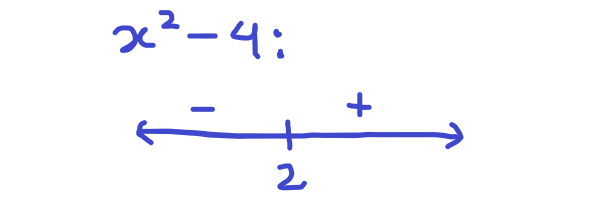
\includegraphics[scale=0.5]{images/prob40}
\end{figure}
This is only possible when $n - 1$ is odd.\\
$\Rightarrow n$ is any even number.
\end{prob}
\pagebreak
\begin{prob}
The least value of $a \in \mathbb{R}$ for which $4ax^2 + \dfrac1{x} \geq 1$ for all $x > 0$ is:\\
\begin{enumerate*}[label=(\Alph*)]
\item $\dfrac1{64}\quad\quad$
\item $\dfrac1{32}\quad\quad$
\item $\dfrac1{27}\quad\quad$
\item $\dfrac1{25}$\\
\end{enumerate*}\\
\textbf{Solution (C):}
\paragraph{Method 1:} Using Calculus\\
Consider the function $f(x) = 4ax^2 + \dfrac1{x}$ in the interval $(0, \infty)$.\\
The problem stipulates that $f(x) \geq 1 \; \forall x \in (0, \infty)$\\
\textbf{Proposition:} If the minimum value of the function is greater than or equal to 1, then it is necessary and sufficient for the condition to be satisfied.
\[f'(x) = 8ax - \dfrac1{x^2}\]
Finding Critical points:
\[8 ax^3 - 1 = 0\]
\[\Rightarrow x^3 = \dfrac1{8a}\]
\[\Rightarrow x = \dfrac1{2(a)^{\frac13}}\]
\begin{figure}[h]
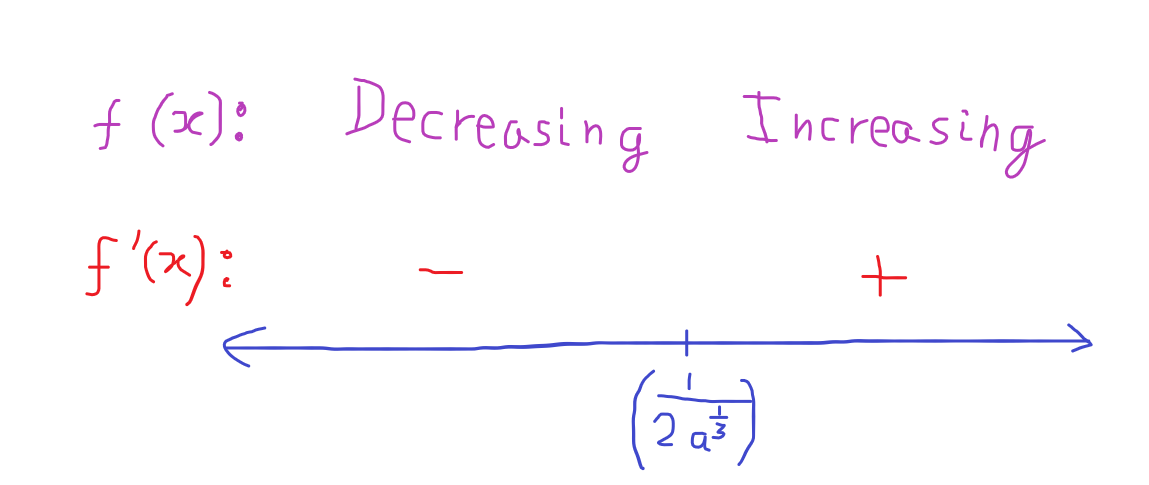
\includegraphics[scale=0.25]{images/prob41}
\end{figure}
Therefore $f(x)$ attains its minimum value at $x = \dfrac1{2(a)^{\frac13}}$, which is $f\left(\dfrac1{2(a)^{\frac13}}\right)$.
\[\Rightarrow f\left(\dfrac1{2(a)^{\frac13}}\right) \geq 1\]
\[\Rightarrow 4a\cdot \left( \dfrac1{2a^{\frac13}}\right)^2 + 2a^{\frac13}\geq 1\]
\[\Rightarrow 3a^{\frac13} \geq 1\]
\[\Rightarrow a^{\frac13} \geq \dfrac1{3}\]
\[\Rightarrow a \geq \left(\dfrac13\right)^3\]
\[\Rightarrow a \geq \dfrac1{27}\]
Therefore, option \textbf{C} is correct.
\pagebreak
\paragraph{Method 2:} Using AM-GM Inequality
\[f(x) = 4ax^2 + \dfrac1{x} \geq 1, \quad x \in (0, \infty)\]
In order to apply the AM-GM inequality, we must ensure that the terms are all non-negative, which will be the case if and only if $a$ is non-negative.\\
\textbf{Claim:} $a \geq 0$
\begin{proof}
Assume for the purpose of contradiction that a is negative.\\
Then,
\[\lim\limits_{x \to \infty} f(x) = \lim\limits_{x \to \infty} 4ax^2 + \dfrac1{x} < 0\]
This contradicts the fact that $f(x) \geq 1 \quad \forall x \in (0, \infty)$\\
Therefore, $a \geq 0$.\\
\end{proof}
Now, applying AM-GM inequality on $4ax^2$, $\dfrac1{2x}$ and $\dfrac1{2x}$
\[4ax^2 + \dfrac1{2x} + \dfrac1{2x} \geq 3 \left( (4ax^2)\left(\dfrac1{2x}\right)\left(\dfrac1{2x}\right) \right)^{\dfrac13}\]
\[\Rightarrow 4ax^2 + \dfrac1{x} \geq 3a^{\frac13}\]
The equality holds when $4ax^2 = \dfrac1{2x}$ or at $x^3 = \dfrac1{8a} \Rightarrow x = \dfrac1{2a^{\frac13}}$, which is permissible.\\
This implies that the minimum value of $f(x)$ is $3a^{\frac13}$, but $f(x) \geq 1 \; \forall x \in (0, \infty)$.\\
\[\Rightarrow 3a^{\frac13} \geq 1\]
\[\Rightarrow a^{\frac13} \geq \dfrac13\]
\[\Rightarrow a \geq \dfrac1{3^3}\]
\[\Rightarrow a \geq \dfrac1{27}\]
Therefore, option \textbf{C} is correct.
\end{prob}
\pagebreak
\begin{prob}
The function $f(x) = 2 \abs{x} + \abs{x + 2} - \abs{\;\abs{x + 2} - 2 \abs{x}}$ has a local minimum or a local maximum at $x$ equal to:\\
\begin{enumerate*}[label=(\Alph*)]
\item $-2\quad\quad\quad\quad$ 
\item $\dfrac{-2}3\quad\quad\quad\quad$
\item $2\quad\quad\quad\quad$
\item $\dfrac23\quad\quad\quad\quad$\\
\end{enumerate*}
\textbf{Solution (AB):}\\
We know that, 
\[\text{max}\{f(x), g(x)\} = \dfrac{f(x) + g(x)}{2} + \dfrac{\abs{f(x) - g(x)}}{2}\]
\[\text{min}\{f(x), g(x)\} = \dfrac{f(x) + g(x)}{2} - \dfrac{\abs{f(x) - g(x)}}{2}\]
Then, \[f(x) = 2 \cdot \text{min}\{\;\abs{x - 2}, 2\abs{x}\}\]
\begin{figure}[h]
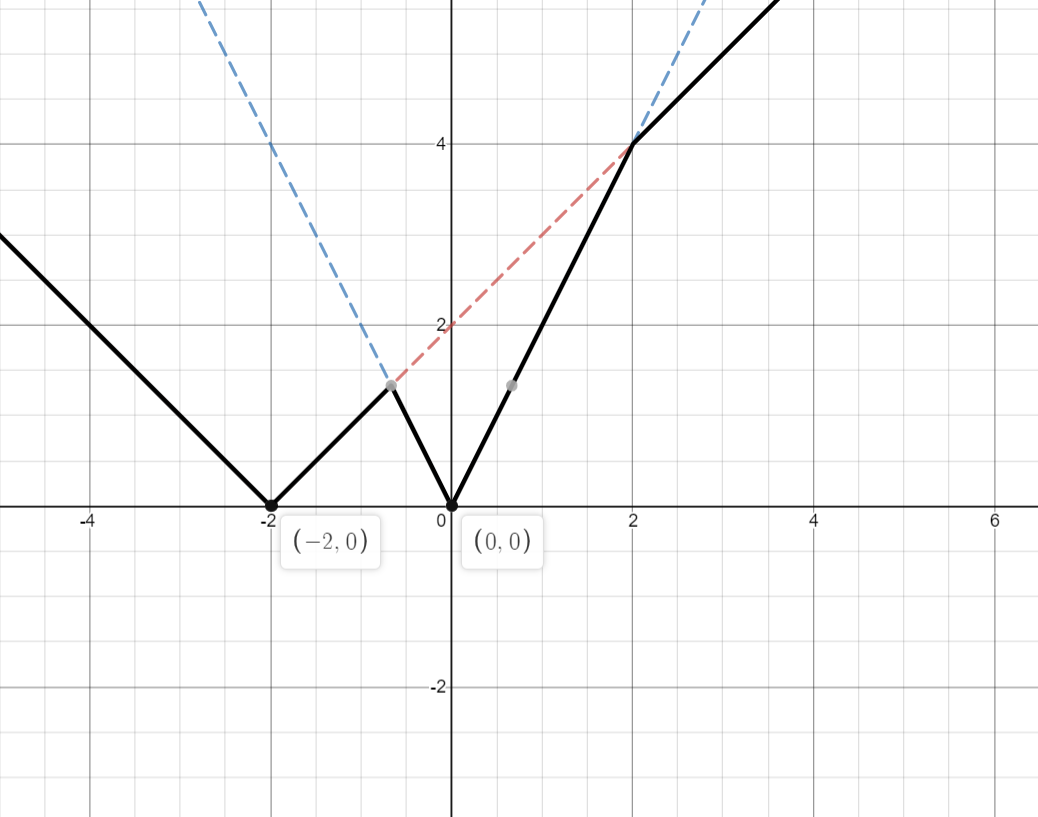
\includegraphics[scale=0.5]{images/prob42}
\end{figure}
We can plot the graph here.\\
The critical points are at $x = -2, -\dfrac23, 0, 2$
\end{prob}
The point at $x=2$ is neither that of a minimum, nor of a maximum, because the derivative is positive both to its immediate left and right.\\
The points of minima are at $x = -2$ and $x = 0$, and the point of maximum is at $x = \dfrac{-2}{3}$.\\
Therefore, options \textbf{(A)} and \textbf{(B)} are correct.
\pagebreak
\begin{prob}
If the roots of the equation $x^4 - 4x^3 + ax^2 + bx + 1 = 0$ are all positive, find the value of $(a - b)$.\\
\textbf{Solution: }
\[x^4 - 4x^3 + ax^2 + bx + 1 = 0\]
Say the roots are $x_1$, $x_2$, $x_3$ and $x_4$.\\
Then,
\[\text{Sum of roots } = x_1 + x_2 + x_3 + x_4 = 4\]
\[\Rightarrow \dfrac{x_1 + x_2 + x_3 + x_4}4 = 1\]
And
\[
\text{Product of roots } = x_1 \cdot x_2 \cdot x_3 \cdot x_4 = 1
\]
\[
\Rightarrow (x_1 \cdot x_2 \cdot x_3 \cdot x_4)^{\frac14} = 1^{\frac14} = 1
\]
That means, AM of the roots $=$ GM of the roots.\\
The equality holds for the AM-GM inequality if and only if all the terms are equal.\\
Therefore,
\[x_1 = x_2 = x_3 = x_4 = 1\]
Then,
\[
a = \text{Sum of roots taken two at a time} = {}^4C_2 = 6
\]
\[
-b = \text{Sum of roots taken three at a time} = {}^4C_3 = 4
\]
\[
\Rightarrow b = -4
\]
\begin{align*}
a - b &= 6 - (- 4)\\
&= 6 + 4\\
&= 10
\end{align*}
Therefore, we get the value of $(a - b)$ as 10.
\end{prob}
\pagebreak
\begin{prob}
Find the total number of points of global maxima of $ f(x) = \cos(x) + \cos(\sqrt{2} x)$\\
\textbf{Solution:}
We know that the maximum value of $\cos(A) + \cos(B)$ can be at most $1$ because the range of $\cos(x)$ is $[-1, 1]$.\\
It is clear that $\cos(x) + \cos(\sqrt2 x)$ will have the value $2$ at $x = 0$. Therefore, $x = 0$ is a point of global maximum.\\
To check if other such points exist, we can solve $\cos(x) = 1$ and $cos(\sqrt2 x) = 1$ simultaneously, which will give us $x = 0$ as the only solution.\\
\end{prob}
\subsection{Concavity}
\begin{define}
A function is said to be (weakly) \underline{concave up} if a line joining any two arbitrary points of the curve lies on or above the curve.
\end{define}
\begin{define}
A function is said to be \underline{strictly concave up} if a line joining any two arbitrary points always lies above the curve.
\end{define}
\begin{define}
A function is said to be (weakly) \underline{concave down} if a line joining any two arbitrary points of the curve lies on or below the curve.
\end{define}
\begin{define}
A function is said to be \underline{strictly concave down} if a line joining any two arbitrary points always lies below the curve.
\end{define}
\subsubsection{Mathematical Condition for a Function to be Concave Up}
\begin{figure}[h]
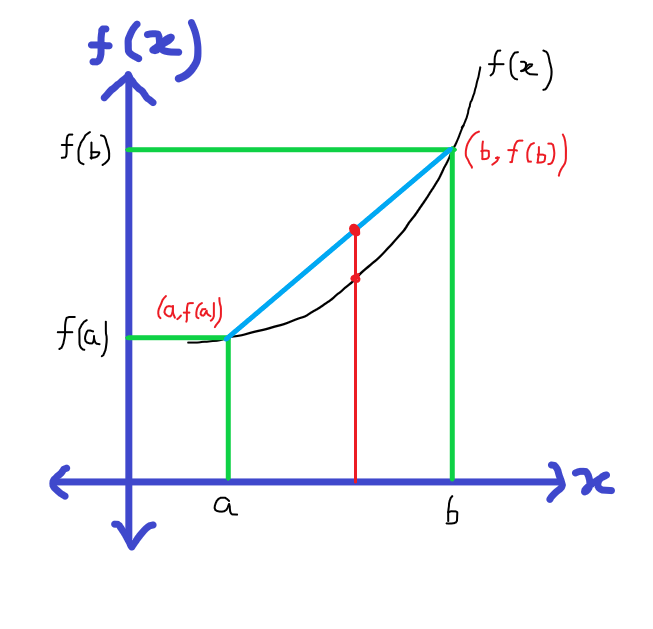
\includegraphics[scale=0.417]{images/concave_up}
\end{figure}
Equation of line joining the points:
\[y - f(a) = \dfrac{f(b) - f(a)}{b - a} (x-a)\]
\[\Rightarrow y = \dfrac{f(b) - f(a)}{b - a} (x-a) + f(a)\]
Condition for concave up:
\[
\dfrac{f(b) - f(a)}{b - a} (x-a) + f(a) \geq f(x)\quad \forall x \in [a, b]
\]
\[\Rightarrow \dfrac{f(b) - f(a)}{b - a} \geq \dfrac{f(x) - f(a)}{x - a} \quad \forall x \in [a, b]\]\\
\pagebreak
Similarly,\\
For strictly concave up:
\[\dfrac{f(b) - f(a)}{b - a} > \dfrac{f(x) - f(a)}{x - a} \quad \forall x \in (a, b)\]
For concave down:
\[\dfrac{f(b) - f(a)}{b - a} \leq \dfrac{f(x) - f(a)}{x - a} \quad \forall x \in [a, b]\]
For strictly concave down:
\[\dfrac{f(b) - f(a)}{b - a} < \dfrac{f(x) - f(a)}{x - a} \quad \forall x \in (a, b)\]
\subsubsection{Properties}
Let $f$ be a differentiable function, then:
\begin{enumerate}
\item If $f$ is concave up in $(a, b)$ then $f'(a) \leq f'(b)$ and $f'$ is non-decreasing.
\item If $f$ is strictly concave up in $(a, b)$ then $f'(a) < f'(b)$ and $f'$ is strictly increasing.
\item If $f$ is concave down in $(a, b)$ then $f'(a) \geq f'(b)$ and $f'$ is non-increasing.
\item If $f$ is strictly concave down in $(a, b)$, then $f'(a) > f'(b)$ and $f'$ is strictly decreasing.
\end{enumerate}
Let $f$ be a twice-differentiable function, then:
\begin{enumerate}
\item $f$ is concave up when $f''(x) \geq 0$.
\item $f$ is strictly concave up when $f''(x) > 0$.
\item $f$ is concave down when $f''(x) \leq 0$.
\item $f$ is strictly concave down when $f''(x) < 0$.
\end{enumerate}
Suppose $f$ is a twice-differentiable function in $(a, b)$ and strictly concave up. If $f(a) = f(b)$, then $f(x) < f(a) \quad \forall x \in (a, b)$
\subsection{Inflection Points}
\begin{define}
A point $c$ is called a \underline{point of inflection} for a function $f$ if:
\begin{enumerate}
\item There exists a tangent at $c$, and
\item $f$ changes its concavity about $c$.
\end{enumerate}
\end{define}
\begin{define}
If $f$ is a doubly-differentiable function, then $c$ is said to be a \underline{point of inflection} when:
\begin{enumerate}
\item There exists a tangent at $c$,
\item $f''(c) = 0$ and
\item $f''(x)$ must change its sign about the point $c$.
\end{enumerate}
\end{define}
\pagebreak
\begin{prob}
For what values of $a$ will the curve $y = x^4 + ax^3 + 3x^2 + 1$ be concave about the entire real number line?\\
\textbf{Solution:}
\[y = x^4 + ax^3 + 3x^2 + 1\]
\[\Rightarrow y' = 4x^3 + 3ax^2 + 6x\]
\[\Rightarrow y'' = 12x^2 + 6ax + 6\]
\[\Rightarrow y'' = 6 \cdot (2x^2 + ax + 1)\]
For the curve to be concave up, $y'' \geq 0 \quad \forall x$.\\
This is only possible when the discriminant of the quadratic is non-positive.\\
\[\Rightarrow a^2 - 8 \leq 0\]
\[\Rightarrow \left(a + 2\sqrt2\right)\left(a - 2\sqrt2\right) \leq 0\]
\[\Rightarrow a \in \left[-2\sqrt2,\; 2\sqrt2\right]\]
\end{prob}
\begin{prob}
What conditions must the coefficients $a, b$ and $c$ satisfy for the curve $f(x) = ax^4 + bx^3 + cx^2 + dx + e$ to have point(s) of inflection?\\
\textbf{Solution:}\\
\[f(x) = ax^4 + bx^3 + cx^2 + dx + e\]
\[f'(x) = 4ax^3 + 3bx^2 + 2cx + d\]
\[f''(x) = 12ax^2 + 6bx + 2c\]
For $f$ to have a point of inflection, $f$ must be differentiable (which it is, because $f$ is a polynomial function), and should have a point $c$ where $f''(c) = 0$ and $f''(x)$ changes sign at $c$.\\
This means the discriminant of the quadratic must be positive.
\[\Rightarrow (6b)^2 - 4(12a)(2c) > 0\]
\[\Rightarrow 36b^2 - 96ac > 0\]
\[\Rightarrow 6b^2 - 16ac > 0\]
\[\Rightarrow 3b^2 - 8ac > 0\]
\[\Rightarrow 3b^2 > 8ac\]
Therefore, for $f$ to have a point of inflection, the coefficients $a$, $b$ and $c$ must satisfy the condition $3b^2 > 4ac$.
\end{prob}
\pagebreak
\subsection{Jensen's Inequality}
Say a function is concave up in an interval $(x_1, x_2)$\\
\begin{figure}[h]
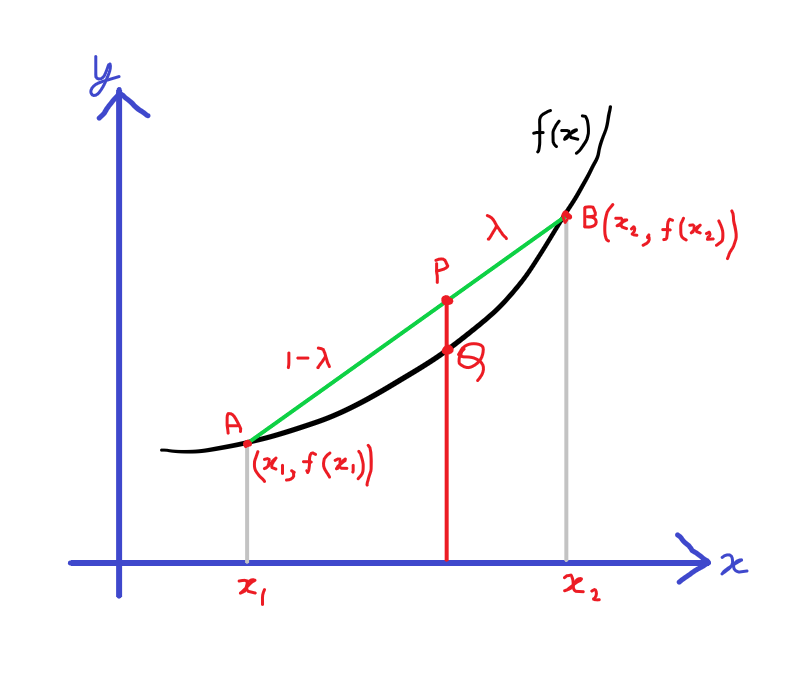
\includegraphics[scale=0.417]{images/jensen}
\end{figure}
Say the point $P$ divides the line segment $AB$ in the ratio $(1 - \lambda):\lambda$\\
Then, using section formula,\\
$P$ will have coordinates 
$\left( \lambda x_1 + (1 - \lambda) x_2,\; \lambda f(x_1) + (1 - \lambda) f(x_2) \right)$.\\
Then, $Q$ will have coordinates $\left( \lambda x_1 + (1 - \lambda) x_2,\; f\left(\lambda x_1 + (1 - \lambda) x_2\right) \right)$\\
As $\lambda$ varies from $0$ to $1$, the point $P$ takes all positions between $A$ and $B$.\\
Since the curve is concave up,\\
$y$-coordinate of $P$ $>$ $y$-coordinate of $Q$
\[\Rightarrow \lambda f(x_1) + (1 - \lambda) f(x_2) > f\left(\lambda x_1 + (1 - \lambda) x_2\right) \]
Say $\lambda = \lambda_1$ and $(1 - \lambda) = \lambda_2$\\
$\lambda_1 > 0, \; \lambda_2 > 0\\ \lambda_1 + \lambda_2 = 1$
\[\Rightarrow \lambda_1 f(x_1) + \lambda_2f(x_2) \geq f\left( \lambda_1 x_1 + \lambda_2x_2 \right)\]
Generalizing,\\
\[\lambda_1 f(x_1) + \lambda_2 f(x_2) + \lambda_3 f(x_3) + \cdots + \lambda_n f(x_n) \geq f\left( \lambda_1 x_1 + \lambda_2 x_2 + \cdots + \lambda_n x_n \right)\]
where $0 < \lambda_i < 1$, $i \in \{1, 2, 3, \cdots, n\}$ and $\lambda_1 + \lambda_2 + \cdots + \lambda_n = 1$\\
This is the general Jensen's inequality for a function that is concave up. The generalization can be proved using Mathematical Induction. However, we are more interested in the special case when $\lambda_1 = \lambda_2 = \cdots = \lambda_n = \dfrac1{n}$.\\
\[\dfrac{f(x_1) + f(x_2) + f(x_3) + \cdots + f(x_n)}{n} \geq f\left(\dfrac{x_1 + x_2 + x_3 + \cdots + x_n}{n}\right)\]
\pagebreak
The sign reverses for a function that is concave down.\\\\
So Jensen's inequality becomes:
\[\dfrac{f(x_1) + f(x_2) + f(x_3) + \cdots + f(x_n)}{n} \geq f\left(\dfrac{x_1 + x_2 + x_3 + \cdots + x_n}{n}\right)\]
if the function is concave up, and
\[\dfrac{f(x_1) + f(x_2) + f(x_3) + \cdots + f(x_n)}{n} \leq f\left(\dfrac{x_1 + x_2 + x_3 + \cdots + x_n}{n}\right)\]
if the function is concave down.
\subsubsection{Proof of the AM-GM Inequality}
\begin{proof}
Consider $f(x) = \ln(x)$. Note that $x > 0$ (from the domain of $f$).\\
\[f'(x) = \dfrac1x\]
\[f''(x) = \dfrac{-1}{x^2}\]
i.e. $f''(x) < 0 \; \forall x > 0$\\
$\Rightarrow f(x) = \ln(x)$ is concave down. Applying Jensen's Inequality:\\
\begin{align*}
\dfrac{f(x_1) + f(x_2) + f(x_3) + \cdots + f(x_n)}{n} &\leq f\left( \dfrac{x_1 + x_2 + x_3 + \cdots + x_n}{n} \right)\\
\dfrac1{n}\left[\ln(x_1) + \ln(x_2) + \ln(x_3) + \cdots + \ln(x_n)\right] &\leq \ln\left( \dfrac{x_1 + x_2 + x_3 + \cdots + x_n}{n} \right)\\
\Rightarrow \dfrac1n \ln \left( x_1 x_2 x_3 \cdots x_n\right)&\leq \ln\left( \dfrac{x_1 + x_2 + x_3 + \cdots + x_n}{n} \right)\\
\Rightarrow \ln \left( (x_1 x_2 x_3 \cdots x_n)^\frac1n \right)&\leq \ln\left( \dfrac{x_1 + x_2 + x_3 + \cdots + x_n}{n} \right)
\end{align*}
Now, since $\ln(x)$ is an increasing function, this means $\ln(x_1) \leq \ln(x_2) \Leftrightarrow x_1 \leq x_2$.
\[\Rightarrow (x_1 x_2 x_3 \cdots x_n)^{\frac1n}\leq \dfrac{x_1 + x_2 + x_3 + \cdots + x_n}{n}\]
\[\Rightarrow\dfrac{x_1 + x_2 + x_3 + \cdots + x_n}{n} \geq (x_1 x_2 x_3 \cdots x_n)^{\frac1n} \]
\[\Rightarrow AM \geq GM\]
\end{proof}
\pagebreak
\subsubsection{Problems}
\begin{prob}
Prove that in a triangle $ABC$, $\sin(A) + \sin(B) + \sin(C) \leq \dfrac{3\sqrt3}{2}$.\\
\begin{proof}
Since $A, B, C$ are angles in a triangle,\\
$0 < A, B, C < \pi$ and $A + B + C = \pi$.\\
Consider the function $f(x) = \sin(x)$ in the interval $[0, \pi].$
\[f(x) = \sin(x)\]
\[f'(x) = \cos(x)\]
\[f''(x) = -\sin(x)\]
\[f''(x) \leq 0 \; \forall x \in [0, \pi]\]
$\sin(x)$ is concave down in $[0, \pi]$. Applying Jensen's Inequality:
\begin{align*}
\dfrac{\sin(A) + \sin(B)+ \sin(C)}{3} &\leq \sin \left( \dfrac{A+B+C}{3} \right)\\
\Rightarrow \dfrac{\sin(A) + \sin(B)+ \sin(C)}{3} &\leq \sin \left( \dfrac{\pi}{3} \right)\\
\Rightarrow \dfrac{\sin(A) + \sin(B)+ \sin(C)}{3} &\leq \dfrac{\sqrt3}{2}\\
\Rightarrow \sin(A) + \sin(B)+ \sin(C) &\leq \dfrac{3\sqrt3}{2}
\end{align*}
\end{proof}
\end{prob}
\begin{prob}
Prove that for an acute-angled triangle $ABC$, $\tan(A) + \tan(B) + \tan(C) \geq 3\sqrt3$
\end{prob}
\begin{proof}
\[A + B + C = \pi\]
\[0 < A, B, C < \dfrac{\pi}2\]
Consider the function $f(x) = \tan(x)$ in the interval $\left[0, \dfrac{\pi}{2}\right)$.
\[f(x) = \tan(x)\]
\[f'(x) = \sec^2(x)\]
\[f''(x) = 2\sec(x)\tan(x) \geq 0 \; \forall x \in \left[ 0, \dfrac{\pi}{2} \right)\]
i.e. $\tan(x)$ is concave up in $\left[0, \dfrac{\pi}{2}\right)$. Applying Jensen's Inequality:
\[\dfrac{\tan(A) + \tan(B) + \tan(C)}{3} \geq \tan \left( \dfrac{A+B+C}{3} \right)\]
\[\Rightarrow \tan(A) + \tan(B) + \tan(C) \geq 3 \tan \left( \dfrac{\pi}{3} \right)\]
\[\Rightarrow \tan(A) + \tan(B) + \tan(C) \geq 3\sqrt3\]
\end{proof}
\pagebreak
\subsection{Problems on Functional Equations}
\begin{prob}
A function $f:\mathbb{R} \to \mathbb{R}$ satisfies the equation $f(x+y) = f(x)\cdot f(y) \; \forall x, y \in \mathbb{R}$ and $f(x) \neq 0$ for any $x$ in $\mathbb{R}$. Let the function be differentiable at $0$ and let $f'(0) = 2$. Find the value of $f(\ln(10))$.\\
\textbf{Solution:}
\[f(x+y) = f(x) \cdot f(y) \; \forall x, y \in \mathbb{R}\]
\[\Rightarrow f(0+0) = f(0) \cdot f(0)\]
\[\Rightarrow f(0) = \left(f(0) \right)^2\]
\[\Rightarrow f(0) = 1 \lor f(0) = 0\]
But $f(x) \neq 0$ for any $x \in \mathbb{R}$ (Given).\\
Therefore,
\[f(0) = 1\]
\fbox{
\parbox{\dimexpr\linewidth-2\fboxsep-2\fboxrule\relax}{
\centering 
\textbf{But why did the problem say that $f(x)$ is never zero?}\\
Suppose $f(0) = 0$\\
Then $f(x+0) = f(x) \cdot f(0) \forall x$\\
Or $f(x) = 0 \; \forall x \in \mathbb{R}$\\
i.e. $f$ will become constant and equal to $0$.\\
In fact, if a function satisfying such a functional equation is zero anywhere, then it's actually zero everywhere.\\
If $f(c) = 0$,
\[f(x+c) = f(x) \cdot f(c) \; =\forall x \in \mathbb{R}\]
\[\Rightarrow f(x+c) = 0 \; \forall x \in \mathbb{R}\]
\[\Rightarrow f(x) = 0 \; \forall x \in \mathbb{R}\]
}
}\\\\
\textbf{Claim 1:} If the function is continuous at $0$, then it is continuous everywhere.
\begin{proof}
$f$ is continuous at 0\\
\[\Rightarrow \lim\limits_{h \to 0} f(h) = f(0) = 1\]
If we can prove that $\lim\limits_{h \to 0} f(x+h) = f(x)$, then we're done.
\[\Rightarrow\lim\limits_{h \to 0} f(x+h) = \lim\limits_{h \to 0} \left( f(x) \cdot f(h) \right) = f(x) \cdot 1 = f(x)\]
\end{proof}
\textbf{Claim 2:} If the function is differentiable at $0$, then it is differentiable everywhere.
\begin{proof}
\[f'(0) =\lim\limits_{h \to 0}  \dfrac{f(h) - f(0)}{h} = \lim\limits_{h \to 0}\dfrac{f(h) - 1}{h} = 2\]
\[f'(x) =\lim\limits_{h \to 0} \dfrac{f(x)\cdot f(h) - f(x)}{h} = \lim\limits_{h \to 0} f(x) \cdot \left( \dfrac{f(h) - 1}{f(h)} \right) = 2f(x)\]
Therefore, it is differentiable everywhere.
\end{proof}
Now,
\[f'(x) = 2f(x)\]
Since we know that $f(x)$ is not zero anywhere, we can divide by $f(x)$.
\[\dfrac{f'(x)}{f(x)} = 2\]
Integrating both sides\\
\[\int\dfrac{f'(x)}{f(x)} \dif x = \int 2 \dif x\]
Let $f(x) = t$. This means $f'(x) \dif x = \dif t$.
\[\Rightarrow \int \dfrac{\dif t}{t} = \int 2\dif x\]
\[\Rightarrow \ln \left(f(x) \right) = 2x + c\]
\[\Rightarrow f(x) = {\rm e}^{2x+c} \]
\[\Rightarrow f(x) = {\rm e}^{2x} \cdot {\rm e}^c\]
But ${\rm e}^c$ is just a constant. Call it $k$.
\begin{align*}
\Rightarrow f(x) &= k {\rm e}^{2x}\\
f(0) &= k{\rm e}^0\\
\Rightarrow f(0) &= k && \text{But } f(0) = 1 \text{ (Given)}\\
\Rightarrow k &= 1\\
\Rightarrow f(x) &= {\rm e}^{2x}
\end{align*}
Now,
\begin{align*}
f\left(\ln(10)\right) &= {\rm e}^{2 \ln(10)}\\
&= {\rm e}^{\ln\left(10^2\right)}\\
&= {\rm e}^{\ln(100)}\\
&= 100
\end{align*}
Therefore, $f\left(\ln(10)\right) = 100$.
\end{prob}
\subsection{Approximations}
\subsubsection{First Order Approximations}
\[f'(x) = \lim\limits_{h \to 0} \dfrac{f(x+h) - f(x)}{h}\]
Say $h = \Delta x$ is sufficiently small.
\[f'(x) \approx \dfrac{f(x + \Delta x) - f(x)}{\Delta x}\]
\[f(x + \Delta x) \approx f(x) + \Delta x f'(x)\]
Higher order approximations can be made using the Taylor Series of the function we're interested in approximating.
\pagebreak
\section{The Antiderivative}
\subsection{The First Fundamental Theorem of Calculus}
\begin{theorem}
Let $f$ be an integrable function in $[a, b]$ and let $F(x) = \displaystyle\int\limits_a^x f(x) \dif x$.Let $f$ be continuous at a point $c \in [a, b]$. Then $F'(c) = f(c)$.
\end{theorem}
In crude terms, it means that the indefinite integral (a.k.a the antiderivative) is the inverse operator of differentiation and does the reverse of that.
\subsection{Definition of the Antiderivative}
\begin{define}
A function $P$ is called the \underline{primitive} (or the \underline{antiderivative}) of a function $f$ in an open interval $I$ if the derivative of $P$ is $f$, i.e. $P'(x) = f(x) \; \forall x \in I$.
\end{define}
\[ F'(x) = f(x) \Rightarrow \int f(x) \dif x = F(x) + c \]
\subsection{Properties of the Antiderivative}
\begin{enumerate}
\item $\displaystyle\int k \cdot f(x) \dif x = k \cdot \displaystyle\int f(x) \dif x$
\item $\displaystyle\int \left[ f(x_1) \pm f(x_2) \pm f(x_3) \pm \cdots \pm f(x_n) \right]\dif x = \displaystyle\int f(x_1) \dif x \pm \displaystyle\int f(x_2) \dif x \pm \cdots \pm \displaystyle\int f(x_n) \dif x$
\item $\displaystyle\int \dfrac{f'(x)}{f(x)}\dif x = \log_{\rm e}\left( \; \abs{f(x)} \right) + c$
\item $\displaystyle\int \left(f(x)\right)^n \cdot f'(x) \dif x = \dfrac{\left[f(x)\right]^{n+1}}{n+1}+c$
\item If $\displaystyle\int f(x) \dif x = F(x)$, then $\displaystyle\int f(ax+b) \dif x = \dfrac{F(ax+b)}{a}+c$
\end{enumerate}
\subsection{Standard Integrals}
\begin{enumerate}
\item $\displaystyle\int x^n \dif x = \dfrac{x^{n+1}}{n+1} + c$, $n \neq -1$
\item $\displaystyle\int \dfrac1x \dif x = \log_{\rm e}\left(\;\abs{x}\right) + c$
\item $\displaystyle\int \dfrac1{x^2} \dif x = -\dfrac1x + c$
\item $\displaystyle\int\sqrt{x} \dif x = \dfrac23 x\sqrt{x} + c$
\item $\displaystyle\int \dfrac1{\sqrt{x}} \dif x =  2\sqrt{x} + c$\pagebreak
\item $\displaystyle\int \cos(x) \dif x = \sin(x) + c$
\item $\displaystyle\int \sin(x) \dif x = -\cos(x) + c$
\item $\displaystyle\int \sec^2(x) \dif x = \tan(x) + c$
\item $\displaystyle\int \sec(x) \tan(x) \dif x = \sec(x) + c$
\item $\displaystyle\int \csc(x) \cot(x) \dif x = -\csc(x) + c$
\item $\displaystyle\int \csc^2(x) \dif x = -\cot(x) + c$
\item $\displaystyle\int \dfrac{\dif x}{x^2 + a^2} = \dfrac1a \tan^{-1}\left(\dfrac{x}{a}\right) + c$
\item $\displaystyle\int \dfrac{\dif x}{x^2 - a^2} = \dfrac1{2a} \log\left(\;\abs{\dfrac{x-a}{x+a}} \right) + c$
\item $\displaystyle\int \dfrac{\dif x}{a^2 -x^2} = \dfrac1{2a} \log\left(\;\abs{\dfrac{a+x}{a-x}} \right) + c$
\item $\displaystyle \int \dfrac{\dif x}{\sqrt{x^2 + a^2}} = \log_{\rm e}\left( \abs{x + \sqrt{x^2 + a^2}}  \right) + c$
\item $\displaystyle \int \dfrac{\dif x}{\sqrt{x^2 - a^2}} = \log_{\rm e} \left( \abs{x + \sqrt{x^2 - a^2}} \right) + c$
\item $\displaystyle \int \dfrac{\dif x}{\sqrt{a^2 - x^2}} = \sin^{-1}\left( \dfrac{x}{a} \right) + c$
\item $\displaystyle \int \dfrac{\dif x}{x \sqrt{x^2 - a^2}} =  \dfrac1{a} \sec^{-1}\left(\;\abs{ \dfrac{x}{a}} \right) + c$
\item $\displaystyle \int \left( \sqrt{x^2 + a^2} 
\right) \dif x = \dfrac{x}{2}\sqrt{x^2 + a^2} + \dfrac{a^2}{2}\log_{\rm e} \left( \abs{x + \sqrt{x^2 + a^2}} \right) + c$
\item $\displaystyle \int \left( \sqrt{x^2 - a^2} 
\right) \dif x = \dfrac{x}{2}\sqrt{x^2 - a^2} - \dfrac{a^2}{2}\log_{\rm e} \left( \abs{x + \sqrt{x^2 - a^2}} \right) + c$
\item $\displaystyle \int \left( \sqrt{a^2 - x^2} \right) \dif x = \dfrac{x}{2}\sqrt{a^2 - x^2} + \dfrac{a^2}{2}\sin^{-1}\left( \dfrac{x}{a} \right) + c$
\end{enumerate}
\pagebreak
\subsection{Integration by Transformation and Adjustment}
\begin{prob}
$\displaystyle\int \dfrac{2 \dif x}{1+ cos(2x)}$
\begin{align*}
I &= \int \dfrac{2 \dif x}{1+ cos(2x)}\\
&= \int \dfrac{\cancel{2}\dif x}{\cancel{2}\cos^2(x) \dif x}\\
&= \int \dfrac{\dif x}{\cos^2(x)}\\
&= \int \sec^2(x) \dif x\\
&= \tan(x) + c
\end{align*}
\end{prob}
\begin{prob}
$\displaystyle\int \dfrac{1}{\sin^2(x) \cos^2(x)} \dif x$
\begin{align*}
I &= \int \dfrac{1}{\sin^2(x) \cos^2(x)} \dif x\\
&= \int \dfrac{\sin^2(x) + \cos^2(x)}{\sin^2(x) \cos^2(x)} \dif x\\
&= \int \dfrac{\cancel{\sin^2(x)}}{\cancel{\sin^2(x)} \cos^2(x)} \dif x + \int \dfrac{\cancel{\cos^2(x)}}{\sin^2(x) \cancel{\cos^2(x)}} \dif x\\
&= \int \sec^2(x) \dif x + \int \csc^2(x) \dif x\\
&= \tan(x) - \cot(x) + c
\end{align*}
\end{prob}
\begin{prob}
$\displaystyle\int \dfrac{x^3 - x^2 + x - 1}{x - 1} \dif x$
\begin{align*}
I &= \int \dfrac{x^3 - x^2 + x - 1}{x - 1} \dif x\\
&= \int \dfrac{x^2 (x-1) + 1(x-1)}{x-1} \dif x\\
&= \int \dfrac{(x^2 + 1)\cancel{(x - 1)}}{\cancel{x-1}} \dif x\\
&= \dfrac{x^3}3 + x + c
\end{align*}
\end{prob}
\pagebreak
\begin{prob}
$\displaystyle\int \cos(x) \cos(2x) \cos(3x) \dif x$
\begin{align*}
I &= \int \cos(x) \cos(2x) \cos(3x) \dif x\\
&= \int \cos(x) \cos(3x) \cos(2x) \dif x\\
&= \dfrac12 \int \left( \cos(4x) + \cos(2x) \right) \cos(2x) \dif x\\
&= \dfrac12 \left[ \int\left( \dfrac{\cos(6x) + \cos(2x)}{2}\right)\dif x + \int \cos^2(2x) \dif x \right]\\
&= \dfrac12 \left[ \dfrac{\sin(6x)}{12} + \dfrac{\sin(2x)}{4} + \int\left( \dfrac{1 + \cos(4x)}{2} \right)\dif x \right]\\
&= \dfrac12 \left[ \dfrac{\sin(6x)}{12} + \dfrac{\sin(2x)}{4} + \dfrac{x}2 + \dfrac{\sin(4x)}{8} \right]+c\\
&= \dfrac14 \left( \dfrac{\sin(6x)}{6} + \dfrac{\sin(2x)}{2} + x + \dfrac{\sin(4x)}{4} \right)+c\\
&= \dfrac14 \left( \dfrac{\sin(6x)}{6} + \dfrac{\sin(2x)}{2} + \dfrac{\sin(4x)}{4} +x \right)+c
\end{align*}
\end{prob}
\begin{prob}
$\displaystyle\int \dfrac{1}{1-\sin(x)} \dif x$
\begin{align*}
I &= \int \dfrac{1}{1-\sin(x)} \dif x && \text{Multiply and divide by the conjugate}\\
&= \int \left( \dfrac{1}{1-\sin(x)} \cdot \dfrac{1+\sin(x)}{1+\sin(x)} \right) \dif x\\
&= \int \dfrac{1 + \sin(x)}{1 - \sin^2(x)}\dif x\\
&= \int \dfrac{1 + \sin(x)}{\cos^2(x)}\dif x\\
&= \int \sec^2(x) \dif x + \int \sec(x) \tan(x) \dif x\\
&= \tan(x) + \sec(x) + c
\end{align*}
\end{prob}
\pagebreak
\begin{prob}
$\displaystyle\int \dfrac{x-1}{x+1} \dif x$
\begin{align*}
I &= \int \dfrac{x-1}{x+1}\dif x\\
&= \int \dfrac{x+1 -1 -1}{x+1} \dif x\\
&= \int \dfrac{x+1-2}{x+1}\dif x\\
&= \int \dfrac{\cancel{x+1}}{\cancel{x+1}} \dif x - 2\int \dfrac{\dif x}{x+1}\\
&= x - 2\log_{\rm e}\left(\; \abs{x+1}\right) + c
\end{align*}
\end{prob}
\begin{prob}
$\displaystyle \int \dfrac{x^2-1}{x^2+1}\dif x$
\begin{align*}
I &= \int \dfrac{x^2-1}{x^2+1}\dif x\\
&= \int \dfrac{x^2 + 1 - 1 - 1}{x^2 + 1} \dif x\\
&= \int \dfrac{\cancel{x^2 + 1}}{\cancel{x^2 + 1}}\dif x - 2 \int \dfrac{\dif x}{1 + x^2}\\
&= x - 2\tan^{-1}(x) + c
\end{align*}
\end{prob}
\pagebreak
\subsection{Integration By Substitution}
This method of integration is sort-of like reverse Chain Rule.\\
Generic Example:\\
Let the antiderivative of $f$ be $F$.
\[\int f\left(g(x)\right) g'(x)\]
Let $g(x) = t$.\\
$\Rightarrow g'(x) \dif x = \dif t$\\
So the integral becomes
\[\int f(t) \dif t = F(t) + c = F\left(g(x)\right) + c\]
If we want to assume $g(x) = t$, first ensure that $g'(x)$ is present along with $\dif x$ in the numerator.
\begin{prob}
$\displaystyle\int \sin^2(x) \cos(x) \dif x$
\end{prob}
\[I = \int \sin^2(x) \cos(x) \dif x\]
Let $\sin(x) = t$\\
$\Rightarrow \cos(x) \dif x = \dif t$
\begin{align*}
\Rightarrow I &= \int t^2 \dif t\\
&= \dfrac{t^3}{3} + c\\
&= \dfrac{\sin^3(x)}{3} + c
\end{align*}
\begin{prob}
$\displaystyle\int x^3 \sin\left( x^4 \right)$
\[I = \int x^3 \sin\left( x^4 \right)\]
Let $x^4 = t$\\
$\Rightarrow 4x^3 \dif x = \dif t$
\begin{align*}
I &= \int \dfrac{\sin(t) \dif t}{4}\\
&= \dfrac14 \int \sin(t) \dif t\\
&= \dfrac{-1}4 \cos(t) + c\\
&= \dfrac{-1}{4}\cos\left(x^4\right)+c
\end{align*}
\end{prob}
\pagebreak
\begin{prob}
$\displaystyle\int \dfrac{\sin(x) + \cos(x)}{\left(\sin(x)-\cos(x)\right)^3}\dif x$
\[I = \int \dfrac{\sin(x) + \cos(x)}{\left(\sin(x)-\cos(x)\right)^3}\dif x\]
Let $\sin(x) - \cos(x) = t$\\
$\Rightarrow \left(\cos(x) + \sin(x)\right) \dif x = \dif t$\\
$\Rightarrow \left(\sin(x)+\cos(x)\right) \dif x = \dif t$
\begin{align*}
I &= \int \dfrac{1}{t^3}\dif t\\
&= \int t^{-3} \dif t\\
&= \dfrac{t^{-3+1}}{-3+1} + c\\
&= \dfrac{t^{-2}}{-2} + c\\
&= \dfrac{\left( \sin(x) - \cos(x) \right)^{-2}}{-2} + c\\
&= \dfrac{-1}{2\left( \sin(x) - \cos(x) \right)^2}+c
\end{align*}
\end{prob}
\begin{prob}
$\displaystyle\int \dfrac{x \dif x}{\left(ax^2 + b\right)^p}$
\[I = \int \dfrac{x \dif x}{\left(ax^2 + b\right)^p}\]
Let $ax^2 + b = t$\\
$\Rightarrow 2ax \dif x = \dif t$\\
$\Rightarrow x \dif x = \dfrac{\dif t}{2a}$
\begin{align*}
I &= \dfrac1{2a} \int \dfrac{1}{t^p}\dif t\\
&= \dfrac1{2a} \int t^{-p} \dif t\\
&= \dfrac1{2a} \cdot \dfrac{t^{(-p+1)}}{-p+1} + c\\
&= \dfrac{t^{(1-p)}}{2a(1-p)}+c
\end{align*}
\end{prob}
\pagebreak
\begin{prob}
$\displaystyle\int \dfrac{\dif x}{{\rm e}^x + {\rm e}^{-x}}$
\begin{align*}
I &= \int \dfrac{\dif x}{{\rm e}^x + {\rm e}^{-x}}\\
&= \int \dfrac{\dif x}{{\rm e}^{-x} \left( 1+ {\rm e}^{2x} \right)}\\
&= \int \dfrac{{\rm e}^{x} \dif x}{1 + {\rm e^{2x}}}
\end{align*}
Let ${\rm e}^x = t$\\
$\Rightarrow {\rm e}^{x} \dif x = \dif t$
\begin{align*}
\Rightarrow I &= \int \dfrac{\dif t}{1 + t^2}\\
&= \tan^{-1}(t) + c\\
&= \tan^{-1}(e^x) + c
\end{align*}
\end{prob}
\begin{prob}
$\displaystyle\int \dfrac{x^3}{\sqrt{x^8 + 1}} \dif x$
\[I = \int \dfrac{x^3}{\sqrt{x^8 + 1}} \dif x\]
Let $x^4 = t$\\
$\Rightarrow 4x^3 \dif x = \dif t$\\
$\Rightarrow x^3 \dif x = \dfrac{\dif t}{4}$
\begin{align*}
I &= \dfrac14 \int\dfrac{1}{\sqrt{t^2 + 1}} \dif t && \text{Using } \int \dfrac{\dif x}{\sqrt{x^2 + a^2}} = \log_{\rm e} \left(\abs{x + \sqrt{x^2 + a^2}} \right) + c\\
&= \dfrac14 \ln\left( \abs{t + \sqrt{t^2 + 1}} \right) + c\\
&= \dfrac14 \ln \left( \abs{x^4 + \sqrt{x^8 + 1}} \right) + c
\end{align*}
\end{prob}
\pagebreak
\begin{prob}
$\displaystyle \int\dfrac{\sec^2(x)}{(\sec(x) + \tan(x))^{\frac32}} \dif x$
\[I = \int \dfrac{\sec^2(x)}{(\sec(x) + \tan(x))^{\frac32}} \dif x\]
Let $\sec(x) + \tan(x) = t$\\
Then $\sec^2(x) - \tan^2(x) = 1$\\
$\Rightarrow \left(\sec(x) + \tan(x) \right)\left( \sec(x) - \tan(x) \right) = 1$\\
$\Rightarrow t\left( \sec(x) - \tan(x) \right) = 1$\\
$\Rightarrow \sec(x) - \tan(x) = \dfrac1t$
\begin{align*}
\sec(x) + \tan(x) &= t\\
\sec(x) - \tan(x) &= \dfrac1t\\
\cline{1-2}
2\sec(x) &= t + \dfrac1t\\
\cline{1-2}
\end{align*}
$\Rightarrow \sec(x) = \dfrac12 \left(t + \dfrac1t\right)$\\
$\sec(x) + \tan(x) = t$\\
$\Rightarrow \sec(x) \left( \sec(x) + \tan(x) \right)\dif x = \dif t$\\
$\Rightarrow \sec(x) \dif x = \dfrac{\dif t}{t}$
\begin{align*}
I &= \bigints \dfrac{\dfrac12 \left( t + \dfrac1t \right) \dfrac{\dif t}{t}}{t^{\frac92}}\\
&=\dfrac12 \bigints \dfrac{ \left( t + \dfrac1t \right) \dfrac{1}{t}}{t^{\frac92}} \dif t =\dfrac12 \bigints \dfrac{ \left( 1 + \dfrac1{t^2} \right)}{t^{\frac92}} \dif t\\
&= \dfrac12 \int t^{\frac{-9}{2}}\dif t + \dfrac12 \int t^{\frac{-13}{2}}\\
&= \dfrac1{\cancel{2}} \left( \dfrac{t^{\frac{-7}{2}}}{\dfrac{-7}{\cancel{2}}}\right) + \dfrac1{\cancel{2}} \left( \dfrac{t^{\frac{-11}{2}}}{\dfrac{-11}{\cancel{2}}} \right) + c = \dfrac{1}{t^{\frac{11}{2}}}\left[\dfrac1{11} + \dfrac1{7}t^2 \right] + c\\
&= \dfrac{-1}{(\sec(x) + \tan(x))^{\frac{11}{2}}}\left[\dfrac1{11} + \dfrac1{7}(\sec(x) + \tan(x))^2 \right] + c
\end{align*}
\end{prob}
\pagebreak
\begin{prob}
$\displaystyle \int \dfrac{x^2 - 1}{x^3 \sqrt{2x^4 - 2x^2 + 1}} \dif x$
\begin{align*}
I &= \int \dfrac{x^2 - 1}{x^3 \sqrt{2x^4 - 2x^2 + 1}} \dif x\\
&= \bigints \left(\dfrac{x^2 - 1}{x^5 \sqrt{2 - \dfrac2{x^2} + \dfrac1{x^4}}}\right) \dif x
\end{align*}
Let $2 - \dfrac2{x^2} + \dfrac{1}{x^4} = t$\\\\
$\Rightarrow 2-2x^{-2} + x^{-4} = t$\\\\
$\Rightarrow \left(4x^{-3} - 4x^{-5}\right) \dif x = \dif t$\\\\
$\Rightarrow \left( \dfrac{1}{x^3} - \dfrac1{x^5}  \right) \dif x = \dfrac{\dif t}{4}$\\\\
$\Rightarrow \left( \dfrac{x^2 - 1}{x^5} \right)\dif x = \dfrac{\dif t}{4}$
\begin{align*}
\Rightarrow I &= \dfrac14 \int \dfrac{\dif t}{\sqrt{t}}\\
&= \dfrac14 \left(2\sqrt{t}\right) + c\\
&= \dfrac{\sqrt{t}}{2} + c\\
&= \dfrac{\sqrt{2x^4 - 2x^2 + 1}}{2} + c
\end{align*}
\end{prob}
\begin{prob}
$\displaystyle \int \dfrac{x^{n-1}}{x^{2n} + a^2} \dif x$
\[I = \int \dfrac{x^{n-1}}{x^{2n} + a^2} \dif x\]
Let $x^n = t$\\\\
$\Rightarrow nx^{n-1} \dif x = \dif t$\\\\
$\Rightarrow x^{n-1} \dif x = \dfrac{\dif t}{n}$
\begin{align*}
\Rightarrow I &= \dfrac1n \int \dfrac{\dif t}{t^2 + a^2}\\
&= \dfrac1a \tan^{-1}\left(\dfrac{t}a \right) + c\\
&= \dfrac1a \tan^{-1}\left(\dfrac{x^n}{a} \right) + c
\end{align*}
\end{prob}
\pagebreak
\begin{prob}
$\displaystyle \int \dfrac{\dif x}{x^2 (x^4 + 1)^{3/4}}$
\begin{align*}
I &= \int \dfrac{\dif x}{x^2 (x^4 + 1)^{3/4}}\\
&= \bigints \dfrac{\dif x}{x^2 \left[ x^4 \left(1 + \dfrac1{x^4} \right) \right]^{3/4}}\\
&= \bigints \dfrac{\dif x}{x^5 \left(1 + \dfrac1{x^4} \right)^{3/4}}
\end{align*}
Let $1 + \dfrac1{x^4} = t$\\\\
$\Rightarrow\dfrac{-4}{x^5} \dif x = \dif t$\\\\
$\Rightarrow \dfrac{\dif x}{x^5} = \dfrac{-\dif t}{4}$
\begin{align*}
\Rightarrow I &= \dfrac{-1}{4} \cdot \int \dfrac{1}{t^{3/4}} \dif t\\
&= \dfrac{-1}4 \cdot \dfrac{t^{\left(-\frac34 + 1\right)}}{\left(-\dfrac34 + 1\right)}+c\\
&= \dfrac{-1}4 \cdot \dfrac{t^{\frac14}}{\dfrac14}+c\\
&= -t^{1/4}+c\\
&= - \left(1 + \dfrac1{x^4} \right)^{1/4}+c\\
&= \dfrac{-(x^4 + 1)^{1/4}}{x}+c
\end{align*}
\end{prob}
\pagebreak
\begin{prob}
$\displaystyle \bigint \dfrac{x^2 - 1}{(x^4 + 3x^2 + 1) \tan^{-1} \left( \dfrac{x^2 + 1}{x} \right)} \dif x$
\begin{align*}
I &= \bigint \dfrac{x^2 - 1}{(x^4 + 3x^2 + 1) \tan^{-1} \left( \dfrac{x^2 + 1}{x} \right)} \dif x\\
&= \bigint \dfrac{1 - \cfrac1{x^2}}{\left[ \left( x + \dfrac1x \right)^2 + 1 \right] \tan^{-1} \left( x + \dfrac1x \right)} \dif x
\end{align*}
Let $x + \dfrac1x = t$\\
$\left( 1 - \dfrac1{x^2} \right) \dif x = \dif t$\\
\[
\Rightarrow I = \int \dfrac{\dif t}{(t^2 + 1) \tan^{-1}(t)}
\]
Let $\tan^{-1} (t) = u$\\
$\Rightarrow \dfrac{\dif t}{1 + t^2} = \dif u$\\
\begin{align*}
\Rightarrow I &= \int \dfrac{\dif u}{u}\\
&= \ln\left(\; \abs{u} \right) + c\\
&= \ln\left(\; \abs{\tan^{-1}(t)} \right) + c\\
&= \ln\left(\; \abs{\tan^{-1}\left(x + \dfrac1x\right)} \right) + c
\end{align*}
\end{prob}
\pagebreak
\begin{prob}
$\displaystyle \int \dfrac{\dif x}{a^2 \sin^2(x) + b^2 \cos^2(x)}$
\begin{align*}
I &= \int \dfrac{\dif x}{a^2 \sin^2(x) + b^2 \cos^2(x)} && \text{Divide numerator and denominator by } \cos^2(x)\\
&= \int \dfrac{\sec^2(x)}{a^2 \tan^2(x) + b^2}\dif x
\end{align*}
Let $\tan(x) = t$\\
$\Rightarrow \sec^2(x) \dif x = \dif t$
\begin{align*}
\Rightarrow I &= \int \dfrac{\dif t}{a^2 t^2 + b^2}\\
&= \dfrac1{a^2} \bigintss \dfrac{\dif t}{t^2 + \dfrac{b^2}{a^2}}\\
&= \dfrac1{a^{\cancel{2}}}\cdot \dfrac1{\left(\dfrac{b}{\cancel{a}}\right)} \tan^{-1}\left[\dfrac{t}{\left(\dfrac{b}{a}\right)}\right]+c\\
&=\dfrac1{ab} \tan^{-1} \left( \dfrac{at}{b} \right)+c\\
&=\dfrac1{ab} \tan^{-1} \left( \dfrac{a\tan(x)}{b} \right)+c
\end{align*}
\end{prob}
\begin{prob}
$\displaystyle \int \dfrac{1}{x\ln(x)}\dif x$
\[I = \int \dfrac1{x \ln(x)} \dif x\]
Let $\ln(x) = t$\\
$\Rightarrow \dfrac1{x} \dif x = \dif t$
\begin{align*}
\Rightarrow I &= \int \dfrac1{t} \dif t\\
&= \ln\left(\;\abs{t}\right) + c\\
&= \ln\left(\; \abs{\ln(x)} \right) + c
\end{align*}
\end{prob}
\pagebreak
\subsection{Integration by Parts}
We know from the product rule that
\[\dfrac{\dif}{\dif x}(uv) = v\dfrac{\dif u}{\dif x} + u \dfrac{\dif v}{\dif x}\]
\[\Rightarrow \dif\; (uv) = v \dif u + u \dif v\]
\[\Rightarrow u \dif v = \dif\; (uv) - v \dif u\]
Integrate both sides\\
\[\Rightarrow \int u \dif v = uv - \int v \dif u\]
We use this result to split the integrand into two ``parts" $u$ and $\dif v$.\\ We differentiate the first part $u$ and integrate the second part $\dif v$. 
\begin{prob}
$\displaystyle\int x \sin(x) \dif x$
\[I = \int x \sin(x) \dif x\]
Let us choose $u = x$ and $\dif v = \sin(x) \dif x$.\\
$\Rightarrow \dif u = \dif x$ and $v =-\cos(x)$
\begin{align*}
\Rightarrow I = \int u \dif v &= uv - \int v \dif u\\
&= -x \cos(x) - \int \left(- \cos(x)\right) \dif x\\
&= -x \cos(x) + \int \cos(x) \dif x\\
&= \sin(x) - x \cos(x) + c
\end{align*}
\end{prob}
\begin{prob}
$\displaystyle \int \sin^{-1}(x) \dif x$
\begin{align*}
I &= \int\sin^{-1}(x) \dif x\\
\end{align*}
Let us choose $u=\sin^{-1}(x)$ and $\dif v=\dif x$.\\
Then $\dfrac1{\sqrt{1 - x^2}} \dif x = \dif u$ and $v = x$
\begin{align*}
\Rightarrow I = \int u \dif v &= uv - \int v \dif u\\
&= x \sin^{-1}(x) - \int \dfrac{x \dif x}{\sqrt{1 - x^2}} && \text{Let } x^2 = t \Rightarrow 2x \dif x = \dif t\\
&= x \sin^{-1}(x) - \dfrac12 \int \dfrac{\dif t}{\sqrt{1 - t}}\\
&= x \sin^{-1}(x) + \dfrac1{\cancel{2}} \cdot \cancel{2}\sqrt{1-t}+c\\
&= x \sin^{-1}(x) + \sqrt{1-t}+c\\
&= x \sin^{-1}(x) + \sqrt{1-x^2}+c
\end{align*}
\end{prob}
\pagebreak
\begin{prob}
$\displaystyle \bigints \left( x - \dfrac1{x^3} \right) {\mathrm{e}}^{\left(x + \dfrac1x\right)} \dif x$
\begin{align*}
I &= \bigints \left( x - \dfrac1{x^3} \right) {\mathrm{e}}^{\left(x + \dfrac1x\right)} \dif x\\
&=\bigints \left(\dfrac{x^4 - 1}{x^3} \right) {\mathrm{e}}^{\left(x + \dfrac1x\right)} \dif x\\
&=\bigints \left(\dfrac{\left(x^2 + 1\right)\left(x^2 - 1\right)}{x^3} \right) {\mathrm{e}}^{\left(x + \dfrac1x\right)} \dif x\\
&= \bigints \left( \left( \dfrac{x^2 + 1}{x} \right) \left( \dfrac{x^2 - 1}{x^2} \right) \right) {\mathrm{e}}^{\left(x + \dfrac1x\right)} \dif x\\
&= \bigints  \left( x + \dfrac1x \right) \left( 1 - \dfrac1{x^2} \right) {\mathrm{e}}^{\left(x + \dfrac1x\right)} \dif x
\end{align*}
Let $x + \dfrac1x = t$, then $\left(1 - \dfrac1{x^2}\right) \dif x = \dif t$
\[\Rightarrow I = \int t \cdot \mathrm{e}^t \dif t\]
This essentially reduces to the next problem but let's just do it twice.\\
Integrating by parts.\\
Let us choose $u = t$ and $\dif v = e^t \dif t$\\
Then $\dif u = \dif t$ and $v = \mathrm{e}^t$
\begin{align*}
I = \int u \dif v &= uv - \int v \dif u\\
&= t\cdot \mathrm{e}^t - \int \mathrm{e}^t \dif t\\
&= t\cdot \mathrm{e}^t - e^t + c && \text{Substitute back}\\
&= {\left(x + \dfrac1x\right)} \cdot \mathrm{e}^{\left(x + \dfrac1x\right)} - \mathrm{e}^{\left(x + \dfrac1x\right)} + c
\end{align*}
\end{prob}
\pagebreak
\begin{prob}
$\displaystyle\int x \cdot {\rm e}^x \dif x$
\end{prob}
\[I = \int x \cdot {\rm e}^x \dif x\]
Integrating by parts.\\
Let us choose $u = x$ and $\dif v = {\rm e}^x \dif x$\\
$\Rightarrow \dif u = \dif x$ and $v = e^x$
\begin{align*}
\Rightarrow I = \int u \dif v &= uv - \int v \dif u\\
&= x\cdot {\rm e}^x - \int {\rm e}^x \dif x\\
&= x\cdot {\rm e}^x - {\rm e}^x + c
\end{align*}
\begin{prob}
$\displaystyle \int {\rm e}^x \cdot x^2 \dif x$
\end{prob}
\[I = \int {\rm e}^x \cdot x^2 \dif x\]
Integrating by parts.\\
Let us choose $u = x^2$ and $\dif v = {\rm e}^x \dif x$\\
Then $\dif u = 2x \dif x$ and $v = {\rm e}^x$\\
\begin{align*}
\Rightarrow I = \int u \dif v &= uv - \int v \dif u\\
&= x^2 \cdot {\rm e}^x - \int {\rm e}^x \cdot (2x \dif x)\\
&= x^2 \cdot {\rm e}^x - 2 \int x \cdot {\rm e}^x \dif x
\end{align*}
Integrating by parts again.\\
Let us choose $p = x$ and $\dif q = {\rm e}^x \dif x$\\
Then $\dif p = \dif x$ and $q = {\rm e}^x$
\begin{align*}
\Rightarrow I = x^2 \cdot {\rm e}^x - 2 \int p \dif q &= x^2 \cdot {\rm e}^x - 2 \left( pq - \int q \dif p \right)\\
&= x^2 \cdot {\rm e}^x - 2 \left( x {\rm e}^x - \int {\rm e}^x \dif x \right)\\
&= x^2 \cdot {\rm e}^x - 2 \left( x {\rm e}^x - {\rm e}^x \right) + c
\end{align*}
Note: We can also solve this problem using the method of indefinite coefficients.
\pagebreak
\subsection{The Method of Indefinite Coefficients}
\subsubsection{For Polynomial Functions}
\textbf{Claim: } Let $P_n(x)$ be a polynomial in $x$ of degree $n$. Then,
\[\int {\rm e}^{ax} P_n(x) \dif x = \rm {\rm e}^{ax} Q_n(x) + c\]
where $Q_n(x)$ is some polynomial in $x$ of degree $n$. 
\begin{prob}
$\displaystyle \int {\rm e}^x \cdot x^2 \dif x$
\[I = \int {\rm e}^x \cdot x^2 \dif x\]
Using the method of indefinite coefficients,\\
\[\int {\rm e}^x \cdot x^2 \dif x = {\rm e}^x \cdot \left(Ax^2 + Bx + C\right) + c\]
for some $A$, $B$ and $C$.\\
Differentiate both sides\\
\[\cancel{{\rm e}^x} \cdot x^2 = \cancel{{\rm e}^x} \left( Ax^2 + Bx + C + 2Ax + B \right)\]
\[\Rightarrow x^2 = Ax^2 + (2A + B)x + (B+C)\]
Comparing coefficients\\
\[A = 1\]
\[2A + B = 0\]
\[B + C = 0\]
\[\Rightarrow B = -2\]
\[\Rightarrow C = 2\]
Therefore,
\[I = {\rm e}^{x} \left(x^2 -2x + 2 \right) + c\]
\end{prob}
\pagebreak
\begin{prob}
$\displaystyle \int {\rm e}^x \cdot \left(x^3 + 3x^2 + 3x + 9\right) \dif x$
\[I = \int {\rm e}^x \cdot \left(x^3 + 3x^2 + 3x + 9\right) \dif x\]
Using the method of indefinite coefficients,\\
\[I = {\rm e}^x \cdot \left(Ax^3 + Bx^2 + Cx + D\right) + c\]
for some $A$, $B$, $C$ and $D$.\\
Differentiate both sides\\
\[\cancel{{\rm e}^x} \left(x^3 + 3x^2 + 3x + 9\right) = \cancel{{\rm e}^x} \left( Ax^3 + Bx^2 + Cx + D + 3Ax^2 + 2Bx + C \right)\]
\[\Rightarrow \left(x^3 + 3x^2 + 3x + 9\right) = Ax^3 + (B + 3A)x^2 + (C + 2B)x + (C + D)\]
Comparing coefficients\\
\[A = 1\]
\[B + 3A = 3 \Rightarrow B = 0\]
\[C + 2B = 3 \Rightarrow C = 3\]
\[C + D = 9 \Rightarrow D = 6\]
Therefore,
\[I = {\rm e}^{x} \left(x^3 + 3x + 6 \right) + c\]
\end{prob}
This idea can be extended to trigonometric functions as well.
\subsubsection{For Trigonometric Functions}
Extending the idea to Trigonometric functions,
\[\int {\rm e}^{ax} \sin(px+q) \dif x = {\rm e}^{ax} \left( A \sin(px+q) + B \cos(px+q) \right) + c\] for some $A$ and $B$.\\
Also,
\[\int {\rm e}^{ax} \cos(px+q) \dif x= {\rm e}^{ax}\left[ A \cos(px +q) + B \sin(px + q) \right] + c\]
for some A and B
\subsection{Integrals of the form $\int {\rm e}^x \left( f(x) + f'(x) \right) \dif x$}
\[\int {\rm e}^x \left( f(x) + f'(x)\right) \dif x = {\rm e}^x f(x) + c\]
\pagebreak
\begin{prob}
$\displaystyle \bigintsss {\rm e}^x \left[ \dfrac{x^2 + 1}{(x + 1)^2} \right]\dif x$
\begin{align*}
I &= \bigintsss {\rm e}^x \left[ \dfrac{x^2 + 1}{(x + 1)^2}\right]\dif x\\
&= \bigintsss {\rm e}^x \left[ \dfrac{x^2 - 1 + 2}{(x + 1)^2}\right]\dif x\\
&=\bigintsss {\rm e}^x \left[ \dfrac{x^2 - 1}{(x + 1)^2} +  \dfrac{2}{(x + 1)^2} \right]\dif x\\
&=\bigintsss {\rm e}^x \left[ \dfrac{\cancel{(x+1)}(x-1)}{(x + 1)^{\cancel{2}}} +  \dfrac{2}{(x + 1)^2} \right]\dif x\\
&=\bigintsss {\rm e}^x \left[ \dfrac{x - 1}{x + 1} +  \dfrac{2}{(x + 1)^2} \right]\dif x
\end{align*}
Now, we can see that $\dfrac{\dif}{\dif x}\left(\dfrac{x-1}{x+1}\right) = \dfrac{x-1 - (x + 1)}{(x+1)^2} = \dfrac2{(x+1)^2}$
\[\Rightarrow I = {\rm e}^x\left(\dfrac{x-1}{x+1}\right) + c\]
\end{prob}
\begin{prob}
$\displaystyle \int {\rm e}^x \left( \dfrac{2+ \sin(2x)}{1+\cos(2x)}\right)\dif x $
\begin{align*}
I &= \int {\rm e}^x \left( \dfrac{2+ \sin(2x)}{1+\cos(2x)}\right)\dif x\\
&= \int {\rm e}^x \left( \dfrac{2+ 2\sin(x)\cos(x)}{1+\cos(2x)}\right)\dif x\\
&= \int {\rm e}^x \left( \dfrac{\cancel{2} \left(1 + \sin(x)\cos(x)\right)}{\cancel{2}\cos^2(x)}\right)\dif x\\
&= \int {\rm e}^x \left(\sec^2(x) + \tan(x)\right)\dif x && \text{Notice that } \dfrac{\dif}{\dif x}\tan(x) = \sec^2(x)\\
&= {\rm e}^x \tan(x) + c
\end{align*}
\end{prob}
\begin{prob}
$\displaystyle \int \left[\ln\left(\ln(x)\right)+ \dfrac1{\ln(x)} \right] \dif x$
\[I = \int \left[\ln\left(\ln(x)\right)+ \dfrac1{\ln(x)} \right] \dif x\]
Let $\ln(x) = t$\\
$\Rightarrow x = {\rm e}^t \\\Rightarrow \dif x = {\rm e}^t \dif t$
\begin{align*}
\Rightarrow I &= \int \left[ \ln(t) + \dfrac1{\ln(t)} \right] {\rm e}^t \dif t\\
&= {\rm e}^t \ln(t) + c\\ &= {\rm e}^{\ln(x)}\cdot \ln(\ln(x)) + c
\end{align*}
\end{prob}
\pagebreak
\subsection{General Formula for Integration by Parts}
\[\int u(x) \cdot v(x) \dif x = u(x)\cdot v_1(x) - u'(x)\cdot v_2(x) + u''(x)\cdot v_3(x) - \cdots + (-1)^{(n-1)} u^{(n-1)}(x)\cdot v_n(x)\; +\; (-1)^n \int u^{(n)}(x) \cdot v_n(x) \dif x \]
Where $u^{(i)}(x) = \dfrac{\dif^{\;i}}{\dif x^i} u(x)$  for $i \in \{1, 2, 3, \cdots n\}$\\
And $v_1(x) = \int v(x) \dif x$,\\ $v_2(x) = \int v_1(x) \dif x,$\\ $\vdots$\\ $v_i(x) = \int v_{i-1}(x) \dif x$ for $i \in \{2, 3, 4, \cdots, n\}$
\begin{prob}
Find a formula for $\displaystyle\int P_n(x)\cdot {\rm e}^{kx} \dif x$ where $P_n(x)$ is a polynomial in $x$ of degree $n$.
\[I = \int P_n(x)\cdot {\rm e}^{kx} \dif x\]
Using the general formula for integration by parts.\\
Let us choose $u(x) = P_n(x)$ and $v(x) = {\rm e}^x $\\
Then $u'(x) = P_n'(x)$, $u''(x) = P_n''(x)$, $\cdots$, $u^{(n)}(x) = P_n^{(n)}(x)$\\
And,\\ 
$v_1(x) = \dfrac{{\rm e}^{kx}}{k}$\\
$v_2(x) = \dfrac{{\rm e}^{kx}}{k^2}$\\
$v_3(x) = \dfrac{{\rm e}^{kx}}{k^3}$\\
$\vdots$\\
$v_i(x) = \dfrac{{\rm e}^{kx}}{k^i} \; \forall i$\\
$\vdots$\\
$v_n(x) = \dfrac{{\rm e}^{kx}}{k^n}$\\
Applying the formula,
\[I = \int P_n(x)\cdot {\rm e}^{kx} \dif x
= P_n(x) \dfrac{{\rm e}^{kx}}{k} - P_n'(x)\dfrac{{\rm e}^{kx}}{k^2}+P_n''(x)\dfrac{{\rm e}^{kx}}{k^3}-\cdots\;+\;(-1)^{n-1} P_n^{(n-1)}(x)\dfrac{{\rm e}^{kx}}{k^n} \;+\; (-1)^n P_n^{(n)}(x)\dfrac{{\rm e}^{kx}}{k^{n+1}}
\]
The advantage of using this formula is that this process will end in exactly $n$ (i.e. finitely many) steps.
\end{prob}
\pagebreak
\subsection{Reduction Formulas}
Reduction formulas are basically just recurrence relations in integrals. Here, we try to express an integral for $n$ in terms of its successor or predecessor.
\begin{prob}
$I_n = \displaystyle \int \dfrac{\dif x}{(x^2 + a^2)^n}$
\[I_n = \int \dfrac{\dif x}{(x^2 + a^2)^n}\]
Integrating by parts,\\
Let $u = \dfrac{1}{(x^2 + a^2)^n}$ and $\dif v = \dif x$\\
$\Rightarrow \dif u = \dfrac{-n(2x) \dif x}{(x^2 + a^2)^{n+1}}$ and $v = x$\\
\begin{align*}
\Rightarrow I_n = \int u \dif v &= uv - \int v \dif u\\
&= \dfrac{x}{(x^2 + a^2)^n} + \int \dfrac{2n(x^2) \dif x}{(x^2 + a^2)^{n+1}}\\
&= \dfrac{x}{(x^2 + a^2)^n} + \int \dfrac{2n(x^2 + a^2 - a^2)}{(x^2 + a^2)^{n+1}}\dif x\\
&= \dfrac{x}{(x^2 + a^2)^n} + \int \dfrac{2n(x^2 + a^2)}{(x^2 + a^2)^{n+1}}\dif x - 2na^2\int \dfrac{\dif x}{(x^2 + a^2)^{n+1}}\\
&= \dfrac{x}{(x^2 + a^2)^n} + \int \dfrac{2n}{(x^2 + a^2)^{n}}\dif x - 2na^2\int \dfrac{\dif x}{(x^2 + a^2)^{n+1}}\\
&= \dfrac{x}{(x^2 + a^2)^n} + 2n \int \dfrac{1}{(x^2 + a^2)^{n}}\dif x - 2na^2\int \dfrac{\dif x}{(x^2 + a^2)^{n+1}}\\
I_n&= \dfrac{x}{(x^2 + a^2)^n} + 2n \cdot I_n - 2na^2\cdot I_{n+1}\\
\Rightarrow 2na^2\cdot I_{n+1} &= \dfrac{x}{(x^2 + a^2)^n} + 2n \cdot I_n - I_n\\
&=\dfrac{x}{(x^2 + a^2)^n} + (2n-1) \cdot I_n\\
\Rightarrow I_{n+1} &= \dfrac1{2na^2} \cdot \left( \dfrac{x}{(x^2 + a^2)^n} \right)+\dfrac{2n-1}{2na^2}\cdot I_n
\end{align*}
\end{prob}
\pagebreak
\begin{prob}
Find a reduction formula for $I_n = \displaystyle \int \left( \ln(x) \right)^n \dif x$\\
\[I_n = \int \left( \ln(x) \right)^n \dif x\]
Integrating by parts,\\
Let us choose $u = \left(\ln(x)\right)^n$ and $\dif v = \dif x$\\
Then, $\dif u = \dfrac{n \left(\ln(x)\right)^{n-1}}{x} \dif x$ and $v = x$.
\begin{align*}
I_n = \int u \dif v &= uv - \int v \dif u\\
&= x \left( \ln(x) \right)^n - \bigintsss \cancel{x} \cdot \dfrac{n \left(\ln(x)\right)^{n-1}}{\cancel{x}} \dif x\\
&= x \left( \ln(x) \right)^n - n \int \left( \ln(x) \right)^{n-1} \dif x\\
&=  x \left( \ln(x) \right)^n - n \cdot I_{n-1}
\end{align*}
So our reduction formula becomes
\[I_n = x \left( \ln(x) \right)^n - n \cdot I_{n-1}\]
\end{prob}
\begin{prob}
$I_n = \displaystyle \int x^{\alpha}\left( \ln(x) \right)^n$\\
Integrating by parts.\\
Choosing $u = \left(\ln(x)\right)^n$ and $\dif v = x^{\alpha} \dif x$\\
Then, $\dif u = \dfrac{n \left(\ln(x)\right)^{n-1}}{x} \dif x$ and $v = \dfrac{x^{(\alpha + 1)}}{(\alpha + 1)}$.
\begin{align*}
\Rightarrow I_n = \int u \dif v &= uv - \int v \dif u\\
&= \left(\ln(x)\right)^n \cdot \dfrac{x^{(\alpha + 1)}}{(\alpha + 1)} - \int \dfrac{x^{(\alpha + 1)}}{(\alpha + 1)} \cdot \dfrac{n \left(\ln(x)\right)^{n-1}}{x} \dif x\\
&= \left(\ln(x)\right)^n \cdot \dfrac{x^{(\alpha + 1)}}{(\alpha + 1)} - \dfrac{n}{\alpha + 1}\int \dfrac{(x^{(\alpha + 1)}) \left(\ln(x)\right)^{n-1}}{x} \dif x\\
&= \left(\ln(x)\right)^n \cdot \dfrac{x^{(\alpha + 1)}}{(\alpha + 1)} - \dfrac{n}{\alpha + 1}\int \dfrac{(x^{(\alpha + 1)}) \left(\ln(x)\right)^{n-1}}{x} \dif x\\
&= \left(\ln(x)\right)^n \cdot \dfrac{x^{(\alpha + 1)}}{(\alpha + 1)} - \dfrac{n}{\alpha + 1}\int x^{\alpha} \left(\ln(x)\right)^{n-1} \dif x\\
&= \left(\ln(x)\right)^n \cdot \dfrac{x^{(\alpha + 1)}}{(\alpha + 1)} - \dfrac{n}{\alpha + 1} \left(I_{n-1}\right)\\
&= \dfrac1{\alpha + 1} \left[ x^{\alpha + 1} \left( \ln(x) \right)^n - n \cdot I_{n-1} \right]
\end{align*}
This gives us the following reduction formula:\\
\[I_n = \dfrac1{\alpha + 1} \left[ x^{\alpha + 1} \left( \ln(x) \right)^n - n \cdot I_{n-1} \right]\]
\end{prob}
\pagebreak
\subsubsection*{The Beta Function}
More about it in Definite Integration. The Beta function actually has the limits of integration from 0 to 1. For now, we're concerned with just the antiderivative and a reduction formula for it.
\begin{prob}
$\beta(m, n) = \displaystyle \int x^m (1-x)^{n-1} \dif x$
\[\beta(m, n) = \int x^m (1-x)^{n-1} \dif x\]
Integrating by parts\\
Let us choose $u = (1-x)^{n-1}$ and $\dif v = x^m \dif x$\\
$\Rightarrow \dif u = -(n-1)(1-x)^{n-2} \dif x$ and $v = \dfrac{x^{m+1}}{m+1}$
\begin{align*}
\Rightarrow \beta(m, n) = \int u \dif v &= uv - \int v \dif u\\
&= (1-x)^{n-1} \cdot \dfrac{x^{m+1}}{m+1}+ \int \dfrac{x^{m+1}}{m+1} (n-1)(1-x)^{n-2} \dif x\\
&= (1-x)^{n-1} \cdot \dfrac{x^{m+1}}{m+1}+ \dfrac{n-1}{m+1} \int x^{m+1}(1-x)^{n-2} \dif x\\
&= (1-x)^{n-1} \cdot \dfrac{x^{m+1}}{m+1}+ \dfrac{n-1}{m+1} \beta(m+1, n-2)\\
\end{align*}
\end{prob}
\subsubsection*{The Gamma Function}
Again, more details in Definite Integration. The Gamma Function actually has limits from $0$ to $\infty$ but for now, we're just concerned with its reduction formula. It is used to extend the idea of factorial to the set of real numbers.
\begin{prob}
$\Gamma(n) = \displaystyle\int x^n {\rm e}^{-x} \dif x$
\[\Gamma(n) = \int x^n {\rm e}^{-x} \dif x\]
Integrating by parts\\
(Note that we are violating the ``ILATE" principle. It is not really a rule and just a matter of what's easy to integrate and differentiate.)\\
Let us choose $u = {\rm e}^{-x}$ and $\dif v = x^n \dif x$\\
$\Rightarrow \dif u = -{\rm e}^{-x} \dif x$ and $v = \dfrac{x^{n+1}}{n+1}$
\begin{align*}
\Gamma(n) = \int u \dif v &= uv - \int v \dif u\\
&= {\rm e}^{-x} \cdot \dfrac{x^{n+1}}{n+1} - \int \dfrac{x^{n+1}}{n+1} \cdot \left(-{\rm e}^{-x}\right) \dif x\\
&= {\rm e}^{-x} \cdot \dfrac{x^{n+1}}{n+1} + \dfrac1{n+1}\int x^{n+1} \cdot {\rm e}^{-x} \dif x\\
&= {\rm e}^{-x} \cdot \dfrac{x^{n+1}}{n+1} + \dfrac1{n+1}\cdot \Gamma(n+1)
\end{align*}
So we get the following reduction formula:
\[\Gamma(n) = \dfrac{x^{n+1}}{n+1} \left({\rm e}^{-x}\right) + \dfrac1{n+1} \Gamma(n+1)\]
\end{prob}
\pagebreak
\begin{prob}
$I_n = \displaystyle \int \left( a^2 - x^2 \right)^n \dif x$
\[I_n = \int \left( a^2 - x^2 \right)^n \dif x\]
Integrating by parts\\
Let us choose $u = \left( a^2 - x^2\right)^n$ and $\dif v = \dif x$\\
$\Rightarrow \dif u = -2nx\left( a^2 - x^2 \right)^{n-1}\dif x$ and $v=x$
\begin{align*}
I_n = \int u \dif v &= uv - \int v \dif u\\
&= x\left( a^2 - x^2\right)^n - \bigintsss x\cdot \left( -2nx\left( a^2 - x^2 \right)^{n-1} \right) \dif x\\
&= x\left( a^2 - x^2\right)^n - \bigintsss 2n\left( a^2 - x^2 + a^2\right)\cdot \left( a^2 - x^2 \right)^{n-1} \dif x\\
&= x\left( a^2 - x^2\right)^n - 2n \bigintsss\left( a^2 - x^2\right)^n \dif x + 2na^2 \int \left( a^2 - x^2 \right)^{n-1} \dif x\\
&= x\left( a^2 - x^2\right)^n - 2n I_n + 2na^2 I_{n-1}
\end{align*}
\[I_n = x\left( a^2 - x^2\right)^n - 2n I_n + 2na^2 I_{n-1}\]
\end{prob}
\begin{prob}
$I_{(n, -m)} = \displaystyle \int \dfrac{\sin^n(x)}{\cos^m(x)} \dif x$
\[I_{(n, -m)} = \int \dfrac{\sin^n(x)}{\cos^m(x)} \dif x\]
\[I_{(n, -m)} = \int\sin^{n-1}(x) \dfrac{\sin(x)}{\cos^m(x)} \dif x\]
Integrating by parts\\
Let us choose $u = \sin^{n-1}(x)$ and $\dif v = \dfrac{\sin(x)}{\cos^m(x)} \dif x$\\
$\Rightarrow \dif u = (n-1)\sin^{n}(x) \cos(x) \dif x$ and $v = \dfrac{\left(\cos(x)\right)^{-m+1}}{-m+1}$
\begin{align*}
I_{(n, -m)} = \int u \dif v &= uv - \int v \dif u\\
&= \dfrac{\sin^{n-1}(x)\cdot \left(\cos(x)\right)^{-m+1}}{m-1} - \dfrac{n-1}{m-1} \int \dfrac{\sin^{n-2}(x)}{\cos^{m-2}(x)}\dif x\\
&= \dfrac{\sin^{n-1}(x)\cdot \left(\cos(x)\right)^{-m+1}}{m-1} - \dfrac{n-1}{m-1} I_{(n-2, -(m-2))}
\end{align*}
This gives us the reduction formula as:
\[I_{(n, -m)}= \dfrac{\sin^{n-1}(x)\cdot \left(\cos(x)\right)^{-m+1}}{m-1} - \dfrac{n-1}{m-1} \left(I_{(n-2, 2-m)}\right)\]
\end{prob}
\pagebreak
\subsection{Integration of Rational Functions and Integration by Partial Fractions}
An expression is said to be rational if it is of the form $\dfrac{P(x)}{Q(x)}$ where $P$ and $Q$ are polynomials.\\
The rational function is said to be \textbf{proper} when the degree of $Q(x)$ is greater than the degree of $P(x)$; otherwise it is called \textbf{improper}.\\
Given an improper rational function as the integrand, our first job is to convert it into a proper or mixed fraction, possibly by long division.\\\\
\textbf{Step 1:} If $deg(P(x)) > deg(Q(x))$, then use long division to convert to mixed fraction, and try to integrate. Proceed to step 2\\
Say from long division, $P(x) = q(x) \cdot Q(x) + r(x)$.
Then,
\[\int \dfrac{P(x)}{Q(x)} \dif x = \int q(x) \dif x + \int \dfrac{r(x)}{Q(x)} \dif x\]
\textbf{Step 2:} Here, we have two cases:\\
\begin{addmargin}[3em]{1em}% 1em left, 2em right
\textbf{Case 1:} If $Q(x)$ is a polynomial of odd degree, then $Q(x)$ will have at least one root. Even if all other roots are non-real conjugates, they can be made into quadratics. Try to factor $Q(x)$ in such a form to get only linear or quadratic factors.\\
\[Q(x) = (x-\alpha)(x^2 + \beta x + \gamma)\cdots\]
\textbf{Case 2:} If $Q(x)$ is a polynomial of even degree, try to factor $Q(x)$. If all roots of $Q(x)$ are non-real, it can be expressed as a product of quadratics.\\
In general, we'll try to factor $Q(x)$ as a product of linear and quadratic expressions.\\
\end{addmargin}
\textbf{Step 3:} Once that is done, we'll try to integrate, possibly by Partial Fractions.\\
\subsubsection{Integration by Partial Fractions}
The idea is to decompose a given rational function into a sum of simpler fractions (called partial fractions) that can be integrated by the techniques discussed earlier.\\
We will separate the discussion into cases depending on the way in which the denominator $Q(x)$ can be factored.\\\\
\textbf{Case 1:} If $Q(x)$ can be expressed as a product of distinct linear factors, such as
\[Q(x) = (x - \alpha_1)(x-\alpha_2)(x-\alpha_3)\cdots (x-\alpha_n)\] then we can find constants $A_i$ for all $i$ such that
\[\dfrac{P(x)}{Q(x)} = \dfrac{A_1}{x-\alpha_1} + \dfrac{A_2}{x-\alpha_2} + \dfrac{A_3}{x-\alpha_3} + \cdots + \dfrac{A_n}{x-\alpha_n}\]\\
\textbf{Case 2:} If $Q(x)$ can be represented as a product of linear or quadratic factors, some of which are repeated, such as,
\[Q(x) = (x-\alpha)^m \left( x^2 + \beta x + \gamma\right)^n\]
Then,

\[\dfrac{P(x)}{Q(x)} = \dfrac{A_1}{x - \alpha} +\dfrac{A_2}{(x- \alpha)^2} + \cdots + \dfrac{A_m}{(x-\alpha)^m} + \dfrac{B_1 x + C_1}{\left( x^2 + \beta x + \gamma\right)} + \dfrac{B_2 x + C_2}{\left( x^2 + \beta x + \gamma\right)^2} + \cdots + \dfrac{B_n x + c_n}{\left( x^2 + \beta x + \gamma\right)^n}\]
Then, we can make a common denominator (LCM) on the right and compare coefficients, giving us a system of equations to solve. Alternatively, we can substitute values that make the variable vanish.
\pagebreak
\begin{prob}
$\displaystyle \int \dfrac{2x-3}{(x-1)(2x-1)} \dif x$
\[I = \int \dfrac{2x-3}{(x-1)(2x-1)} \dif x\]
\begin{align*}
\text{Let } \dfrac{2x-3}{(x-1)(2x-1)} &= \dfrac{A}{x-1} + \dfrac{B}{2x-1}\\
&=\dfrac{A(2x-1) + B(x-1)}{(x-1)(2x-1)}\\
\Rightarrow 2x-3 &= A(2x-1) + B(x-1)
\end{align*}
Substitute $x=1$\\
$\Rightarrow 2-3 = A(2-1) \Rightarrow A = -1$\\
Substitute $x = \dfrac12$\\
$\Rightarrow B = 4$
\begin{align*}
\Rightarrow I &= \int \left( \dfrac{-1}{x-1} + \dfrac4{2x-1} \right) \dif x\\
&= -\int \dfrac{\dif x}{x-1} + 4\int \dfrac{\dif x}{2x-1}\\
&= -\ln\left(\; \abs{x-1} \right) + \dfrac{4 \ln \left(\; \abs{2x-1} \right)}{2}+c\\
&= -\ln\left(\; \abs{x-1} \right) + 2 \ln \left(\; \abs{2x-1} \right)+c
\end{align*}
\end{prob}
\pagebreak
\subsection{Integration of Irrational Functions}
\subsubsection{Type 1:}
$\displaystyle \int \dfrac{\dif x}{\text{linear} \sqrt{\text{linear}}}$\\
If you see something of this form, substitute $\sqrt{\text{linear}} = t$.\\
Why? It will give us $\dfrac{\dif x}{2\sqrt{\text{linear}}} = \dif t$. Then, we can express the linear part outside the square root in terms of $t$ and integrate.
\begin{prob}
$\displaystyle \int \dfrac{\dif x}{(2x+3)\sqrt{x+1}}$
\[I =\int \dfrac{\dif x}{(2x+3)\sqrt{x+1}}\]
Let $\sqrt{x+1} = t$\\
$\Rightarrow \dfrac{\dif x}{2\sqrt{x+1}} = \dif t$\\
$\Rightarrow \dfrac{\dif x}{\sqrt{x+1}} = 2\dif t$\\\\
$x + 1 = t^2$\\
$\Rightarrow 2x + 2 = 2t^2$\\
$\Rightarrow 2x + 3 = 2t^2 + 1$\\
\begin{align*}
\Rightarrow I &= \int \dfrac{2\dif t}{2t^2 + 1}\\
&= \bigints \dfrac{\cancel{2} \dif t}{\cancel{2}\left( t^2 + \dfrac12 \right)}\\
&= \dfrac{1}{\left(\dfrac{1}{\sqrt2}\right)}\tan^{-1}\left(\dfrac{t}{\left(\dfrac{1}{\sqrt2}\right)}\right) + c\\
&= \sqrt2 \tan^{-1}\left(\sqrt{2} t\right) + c\\
&= \sqrt2 \tan^{-1}\left(\sqrt{2} \cdot \sqrt{x+1}\right) + c\\
&= \sqrt2 \tan^{-1}\left(\sqrt{2(x+1)}\right) + c
\end{align*}
\end{prob}
\pagebreak
\subsubsection{Type 2:}
$\displaystyle \int \dfrac{\dif x}{(ax^2 + b)\sqrt{cx^2 + d}}$\\
For integrals of this type, substitute $x = \dfrac1{t}$.\\
This will give us $\dif x = -\dfrac1{t^2} \dif t$.
\begin{prob}
$\displaystyle \int \dfrac{\dif x}{(x^2 + 1)\sqrt{x^2 + 2}}$
\[I = \int \dfrac{\dif x}{(x^2 + 1)\sqrt{x^2 + 2}}\]
Let $x = \dfrac1{t}$.\\
$\Rightarrow \dif x = -\dfrac1{t^2} \dif t$
\begin{align*}
\Rightarrow I &= - \bigint \dfrac{\dfrac{\dif t}{t^2}}{\left( \dfrac1{t^2} + 1 \right) \sqrt{\dfrac1{t^2} + 2}}\\
&= - \bigint \dfrac{\dfrac{\dif t}{\cancel{t^2}}}{\left( \dfrac{t^2 + 1}{\cancel{t^2}} \right) \sqrt{\dfrac{1 + 2t^2}{t^2}}}\\
&= - \int \dfrac{t \dif t}{(t^2 + 1)\sqrt{1 + 2t^2}}
\end{align*}
Let $1 + 2t^2 = u^2$\\
$\Rightarrow 4t\dif t = 2u\dif u$\\
$\Rightarrow t \dif t = \dfrac{u \dif u}2$\\
Now $1 + 2t^2 = u^2$\\
$\Rightarrow 2t^2 = u^2 - 1$\\
$\Rightarrow t^2 = \dfrac{u^2 - 1}{2}$\\
$\Rightarrow t^2 + 1 = \dfrac{u^2 - 1}{2} + 1 = \dfrac{u^2 + 1}2$
\begin{align*}
\Rightarrow I &= -\dfrac1{\cancel{2}} \bigintss \dfrac{\cancel{u} \dif u}{\left(\dfrac{u^2 + 1}{\cancel{2}}\right)\cancel{u}} = -\int \dfrac{\dif u}{u^2 + 1}\\
&= - \tan^{-1}(u) + c\\
&= - \tan^{-1}(1 + 2t^2) + c\\
&= - \tan^{-1}\left(1 + \dfrac2{x^2}\right) + c\\
\end{align*}
\end{prob}
\pagebreak
\subsubsection{Type 3:}
$\displaystyle \int \dfrac{\dif x}{\text{linear} \sqrt{\text{quadratic}}}$\\
For this type, we substitute $\text{linear} = \dfrac1t$.                                                                                                                                                                                                                                                                                                                                                                                                                                                                                                                                                                                                                                                                                                                                                                                                                                                                                                                                                                                                                                                                                                                                                                                                                                                                                                                                                                                                                                                                                                                                                                                                                                                                                                                                                                                                                                                                                                                                                                                                                                                                                                                                                                                                                                 
\begin{prob}
$\displaystyle \int \dfrac{\dif x}{(x+2)\sqrt{x^2 + 6x + 7}}$
\[I = \int \dfrac{\dif x}{(x+2)\sqrt{x^2 + 6x + 7}}\]
Let $x + 2 = \dfrac1t$\\
$\Rightarrow \dif x = - \dfrac1{t^2} \dif t$\\\\
And $x = \left(\dfrac1t - 2\right)$\\
$\Rightarrow x^2 + 6x + 7 = \left(\dfrac1t - 2\right)^2 + 6\left(\dfrac1t - 2\right) + 7 = \dfrac{1 + 2t - t^2}{t^2}$
\begin{align*}
\Rightarrow I &= \bigint \dfrac{- \dfrac1{t^2} \dif t}{\dfrac1t \sqrt{\dfrac{1 + 2t - t^2}{t^2}}}\\
&= -\int \dfrac{\dif t}{\sqrt{1 + 2t - t^2}}\\
&= - \int\dfrac{\dif t}{\sqrt{2-(t-1)^2}}\\
&= - \sin^{-1}\left(\dfrac{\sqrt2}{(t-1)}\right) + c\\
&= \sin^{-1}\left(\dfrac{\sqrt2}{(1-t)}\right) + c
\end{align*}
\end{prob}
\pagebreak
\subsubsection{Type 4:}
If there is a polynomial function of the form\\
$f\left(x, x^{p_1/q_1}, x^{p_2/q_2} + x^{p_3/q_3} + \cdots + x^{p_r/q_r}\right)$,\\
Then substitute $x = t^s$ where $s = LCM\left( q_1, q_2, q_3, \cdots, q_r\right)$.\\
Similarly, if we have\\
$f\left(x, (ax+b)^{p_1/q_1}, (ax+b)^{p_2/q_2} + (ax+b)^{p_3/q_3} + \cdots + (ax+b)^{p_r/q_r}\right)$\\
Then substitute $(ax+b) = t^s$ where $s = LCM\left( q_1, q_2, q_3, \cdots, q_r\right)$.\\
This will make it a rational function which can be evaluated.
\begin{prob}
$\displaystyle \int \dfrac{x + x^{2/3} + x^{1/6}}{x (1 + x^{1/3})} \dif x$
\[I = \int \dfrac{x + x^{2/3} + x^{1/6}}{x (1 + x^{1/3})} \dif x\]
Let $x = t^6$\\
$\Rightarrow \dif x = 6t^5 \dif t$
\begin{align*}
\Rightarrow I &= \int\dfrac{6t^5 \left( t^6 + t^4 + t \right)}{t^6 \left( 1 + t^2 \right)} \dif t\\
&= 6 \int \dfrac{t^6 + t^4 + t}{t\left( 1 + t^2 \right)} \dif t && \text{Long division}\\
&= 6 \int \left[ t^3 + \dfrac1{t^2 + 1} \right] \dif t\\
&= 6 \left[ \dfrac{t^4}{4} + \tan^{-1}(t) \right] + c\\
&= 6 \left[ \dfrac{x^{4/6}}{4} + \tan^{-1}(x^{1/6}) \right] + c\\
&= \dfrac32 x^{2/3} + 6 \tan^{-1}\left( x^{1/6} \right) + c\\
\end{align*}
\end{prob}
\subsubsection{Type 5:}
Integrals of the type $\displaystyle \int x^m \left( a + bx^n \right)^p \dif x$\\
\begin{enumerate}
\item If $m$ and $p$ are positive integers, simply use Binomial Theorem and evaluate.
\item If $p$ is an integer but $m$ and $n$ are not integers (but rational), then substitute $x = t^s$ where $s$ is the $LCM$ of the denominators of $m$ and $n$.
\item If $m$ and $p$ are not integers but $\dfrac{m+1}n$ is an integer, then substitute $a + bx^n = t^s$ where $s$ is the denominator of the fraction $p$.
\item If $m$ and $p$ are not integers but $\dfrac{m+1}n + p$ is an integer, then put $ax^{-n} + b = t^s$ where $s$ is the denominator of the fraction $p$.
\end{enumerate}
\pagebreak
\subsection{Other ``Special" Integrals}
\subsubsection{When the Denominator is a Quadratic in $x^2$}
Divide the numerator and denominator by $x^2$ and try to make some substitution from here.
\begin{prob}
$\displaystyle \int \dfrac{x^2 + 1}{x^4 + 1} \dif x$
\begin{align*}
I &= \int \dfrac{x^2 + 1}{x^4 + 1} \dif x\\
&= \bigints \left(\dfrac{1 + \dfrac1{x^2}}{x^2 + \dfrac1{x^2}}\right) \dif x
\end{align*}
Let $x - \dfrac1{x} = t$.\\
Then $\left(1 + \dfrac1{x^2}\right) \dif x = \dif t$\\
$\left( x - \dfrac1{x} \right)^2 = t^2$\\
$\Rightarrow x^2 - 2 + \dfrac1{x^2} = t^2$\\
$\Rightarrow x^2 + \dfrac1{x^2} = t^2 + 2$
\begin{align*}
\Rightarrow I &= \int \dfrac{\dif t}{t^2 + 2}\\
&= \int \dfrac{\dif t}{\left( \sqrt2 \right)^2 + t^2}\\
&= \dfrac1{\sqrt2} \tan^{-1} \left(\dfrac{t}{\sqrt 2} \right) + c\\
&= \dfrac1{\sqrt2} \tan^{-1} \left(\dfrac{\left(x - \dfrac1{x}\right)}{\sqrt 2} \right) + c
\end{align*}
\end{prob}
\pagebreak
\begin{prob}
$\displaystyle \int \dfrac{x^2 - 1}{x^4 + 1} \dif x$
\begin{align*}
I &= \int \dfrac{x^2 - 1}{x^4 + 1} \dif x\\
&= \bigints \left(\dfrac{1 - \dfrac1{x^2}}{x^2 + \dfrac1{x^2}}\right) \dif x
\end{align*}
Let $x + \dfrac1{x} = t$.\\
Then $\left(1 - \dfrac1{x^2}\right) \dif x = \dif t$\\
$\left( x + \dfrac1{x} \right)^2 = t^2$\\
$\Rightarrow x^2 + 2 + \dfrac1{x^2} = t^2$\\
$\Rightarrow x^2 + \dfrac1{x^2} = t^2 - 2$
\begin{align*}
\Rightarrow I &= \int \dfrac{\dif t}{t^2 - 2}\\
\Rightarrow I &= \int \dfrac{\dif t}{t^2 - \left( \sqrt2 \right)^2}
\end{align*}
Using $\displaystyle\int \dfrac{\dif x}{x^2 - a^2} = \dfrac1{2a} \log\left(\;\abs{\dfrac{x-a}{x+a}} \right) + c$
\[\Rightarrow I = \dfrac1{2\sqrt2} \ln\left(\;\abs{\dfrac{t-\sqrt2}{t+\sqrt2}} \right) + c\]
\[\Rightarrow I = \dfrac1{2\sqrt2} \ln\left(\;\abs{\dfrac{x + \dfrac1{x}-\sqrt2}{x + \dfrac1{x}+\sqrt2}} \right) + c\]
\end{prob}
\pagebreak
\subsubsection{Special Integrals Involving Sine and Cosine}
\subsubsection*{Integrals of the form $\displaystyle\int \sin^m(x) \dif x$ or $\displaystyle \int \cos^m (x) \dif x$, where $m \in \mathbb{Z}$}
If $m$ is even:\\
\indent\indent Use $\sin^2(x) = \dfrac{1-\cos(2x)}{2}$ or $\cos^2(x) = \dfrac{1 + \cos(2x)}{2}$\\\\
Otherwise, if $m$ is odd:\\
\indent\indent Break it into power 1 and the nearest even power and use one of the following:\\
\indent\indent\indent\indent $\sin^2(x) = 1-\cos^2(x)$ and substitute $\cos(x) = t$\\
\indent\indent\indent\indent Or $\cos^2(x) = 1-\sin^2(x)$ and substitute $\sin(x) = t$
\begin{prob}
$\displaystyle \int \sin^4(x) \dif x$
\begin{align*}
I &= \int \sin^4(x) \dif x\\
&= \int \left( \sin^2(x) \right)^2 \dif x\\
&= \int \left( \dfrac{1-\cos(2x)}{2} \right)^2 \dif x\\
&= \dfrac14 \int \left( 1 - 2\cos(2x) + \cos^2(x) \right)\dif x\\
&= \dfrac14\int \dif x - \dfrac12 \int\cos(2x) \dif x + \dfrac14 \int \cos^2(2x) \dif x\\
&= \dfrac{x}{4} - \dfrac12 \cdot \dfrac{\sin(2x)}2 + \dfrac14 \int \dfrac{1 + cos(4x)}{2} \dif x\\
&=\dfrac{x}{4} - \dfrac12 \cdot \dfrac{\sin(2x)}2 + \dfrac18 \displaystyle \int \left(1 + \cos(4x)\right) \dif x\\
&=\dfrac{x}{4} - \dfrac12 \cdot \dfrac{\sin(2x)}2 + \dfrac18 \left( x + \dfrac{\sin(4x)}{4} \right) + c\\
&= \dfrac{x}4 - \dfrac{\sin(2x)}{4} + \dfrac{x}8 + \dfrac{\sin(4x)}{32} + c\\
&= \dfrac{12x}{32} - \dfrac{\sin(2x)}{4}+ \dfrac{\sin(4x)}{32} + c\\
&= \dfrac{12x - 8\sin(2x) + \sin(4x)}{32} + c
\end{align*}
\end{prob}
\pagebreak
\begin{prob}
$\displaystyle \int \cos^5(x) \dif x$
\begin{align*}
I &= \int \cos^5(x) \dif x\\
&= \int \cos(x) \cdot \cos^4(x) \dif x\\
&= \int \cos(x) \cdot \left(\cos^2(x)\right)^2 \dif x\\
&= \int \cos(x) \cdot \left( 1 - \sin^2(x) \right)^2 \dif x
\end{align*}
Let $\sin(x) = t$\\
$\Rightarrow \cos(x) \dif x = \dif t$
\end{prob}
\begin{align*}
\Rightarrow I &= \int \left( 1 - t^2 \right)^2 \dif t\\
&= \int \left( 1 -2t^2 + t^4 \right) \dif t\\
&= t -\dfrac{2t^3}{3} + \dfrac{t^5}{5} + c\\
&= \sin(x) - \dfrac{2\sin^3(x)}{3} + \dfrac{\sin^5(x)}{5} + c
\end{align*}
\subsubsection*{Integrals of the form $\displaystyle\int \sin^m(x) \cdot \cos^n(x) \dif x$, where $m,n \in \mathbb{Z}^+$}
If any of $m$ and $n$ is/are odd:\\
\indent \indent Break the (least) odd power to nearest even like before and use one of the following:\\
\indent\indent\indent\indent $\sin^2(x) = 1-\cos^2(x)$ and substitute $\cos(x) = t$\\
\indent\indent\indent\indent Or $\cos^2(x) = 1-\sin^2(x)$ and substitute $\sin(x) = t$\\\\
Else if $m$ = $n$, i.e. $\displaystyle \int sin^m(x) \cos^m(x) \dif x$:\\
\indent \indent Multiply and divide by $2^m$ and try to solve like before.
\subsubsection*{Integrals of the form $\displaystyle\int \sin(mx) \cdot \sin(nx) \dif x$, $\displaystyle\int \cos(mx) \cdot \cos(nx) \dif x$ or $\displaystyle\int \sin(mx) \cdot \cos(nx) \dif x$, where $m,n \in \mathbb{R}^+$}
Multiply and divide by 2; use the transformation formulae from trigonometry to split them into sum/difference of sine and cosine.
\pagebreak
\section{Definite Integrals}
\subsection{The Second Fundamental Theorem of Calculus}
\begin{theorem}
Let $f$ be a continuous function on $[a, b]$ and $f(x) = g'(x) \quad \forall x \in [a,b]$. Then,
\[\int\limits_a^b f(x) \dif x = \int\limits_a^b f = g(b) - g(a)\]
\end{theorem}
\subsection{Geometrical Interpretation}
Let $f$ be a non-negative function on the closed interval $[a, b]$. Then the integral $\displaystyle \int\limits_a^b f(x) \dif x = R(f, a, b)$ represents the area bounded by the function $f$, the lines $x = a$, $x = b$ and the $x$-axis.
\begin{figure}[h]
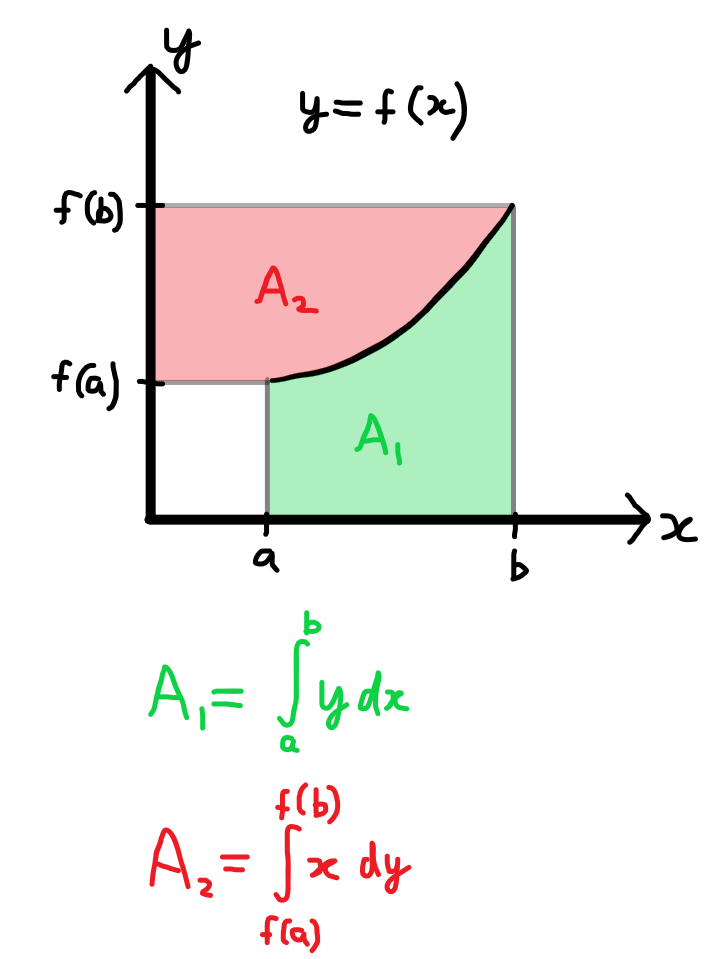
\includegraphics[scale=0.5]{images/integral_area}
\end{figure}
\pagebreak
\subsection{Examples}
\begin{prob}
$\displaystyle \int\limits_0^{\dfrac{\pi}{2}} \sin(2x) \dif x$
\[\int\limits_0^{\pi/2} \sin(2x) \dif x = \left[ \dfrac{-\cos(2x)}{2} \right]_0^{\pi/2} = -\dfrac{\cos(\pi)}{2} + \dfrac{\cos(0)}{2} = \dfrac{-(-1)}{2} + \dfrac12 = 1 \]
\end{prob}
\begin{prob}
$\displaystyle \int\limits_{\dfrac{\pi}6}^{\dfrac{\pi}2} \dfrac{\cos(x)}{\sin^3(x)} \dif x $
\end{prob}
\[I = \int\dfrac{\cos(x)}{\sin^3(x)} \dif x \]
Let $\sin(x) = t$\\
$\Rightarrow \cos(x) \dif x = \dif t$\\
\[I = \int \dfrac{\dif t}{t^3} = \dfrac{t^{-2}}{-2} + c = \dfrac{\left( \sin(x) \right)^{-2}}{-2} + c\]
So,
\[\displaystyle \int\limits_{\pi/6}^{\pi/2} \dfrac{\cos(x)}{\sin^3(x)} \dif x = \left[ \dfrac{\left(\sin(x)\right)^{-2}}{-2}   \right]_{\pi/2}^{\pi/6} = \left[ \dfrac{-1}{2\sin^2(x)} \right]_{\pi/2}^{\pi/6} = \dfrac{-1}{2\sin^2\left(\dfrac{\pi}{6} \right)} + \dfrac1{2\sin^2\left( \dfrac{\pi}{2} \right)} = -2 + \dfrac12 = -\dfrac32\]
\begin{prob}
$\displaystyle \int\limits_0^2 \dfrac{\dif x}{\sqrt{16 - x^2}}$
\[\int\limits_0^2 \dfrac{\dif x}{\sqrt{16 - x^2}} = \int\limits_0^2 \dfrac{\dif x}{\sqrt{4^2 - x^2}} = \left[ \sin^{-1}\left(\dfrac{x}4 \right) \right]_0^2 = \sin^{-1}\left(\dfrac12 \right) - \sin^{-1}(0) = \dfrac{\pi}{6}\]
\end{prob}
\pagebreak
\subsection{Properties of Definite Integrals}
\begin{enumerate}
\item $\displaystyle \int\limits_a^a f(x) \dif x = 0$
\item $\displaystyle \int\limits_a^b f(x) \dif x = \displaystyle \int\limits_a^b f(t) \dif t$
\item $\displaystyle \int\limits_a^b f(x) \dif x = - \displaystyle \int\limits_b^a f(x) \dif x$
\item $\displaystyle \int\limits_a^b f(x) \dif x = \displaystyle \int\limits_a^c f(x) \dif x + \displaystyle \int\limits_c^b f(x) \dif x$
\item $\displaystyle \int\limits_a^b f(x) \dif x = \displaystyle \int\limits_a^{c_1} f(x) \dif x + \displaystyle \int\limits_{c_1}^{c_2} f(x) \dif x + \displaystyle \int\limits_{c_2}^{c_3} f(x) \dif x + \cdots +  \displaystyle \int\limits_{c_n}^{b} f(x) \dif x$
\item $\displaystyle \int\limits_a^b f(x) \dif x = \displaystyle \int\limits_a^b f(a+b-x) \dif x$
\item $\displaystyle \int\limits_0^a f(x) \dif x = \displaystyle \int\limits_0^a f(a-x) \dif x$
\item $\displaystyle \int\limits_0^{2a} f(x) \dif x= \displaystyle \int\limits_0^a f(x) \dif x + \displaystyle \int\limits_0^a f(2a-x) \dif x$
\item $\displaystyle \int\limits_0^{2a} f(x) \dif x = \begin{cases}
      2\displaystyle\int\limits_0^a f(x) \dif x & \text{if }f(2a-x)=f(x) \\
      0 & \text{if }f(2a-x)=-f(x)
\end{cases}\, $
\item $\displaystyle\int\limits_{-a}^a f(x) \dif x = \int\limits_0^a \left[ f(x) + f(-x) \right] \dif x$
\item $\displaystyle \int\limits_{-a}^{a} f(x) \dif x = \begin{cases}
      2\displaystyle\int\limits_0^a f(x) \dif x & \text{if }f(-x)=f(x) \text{ (even function)} \\
      0 & \text{if }f(-x)=-f(x) \text{ (odd function)}
\end{cases}\, $
\item If $f(x)$ is a periodic function with period $T$, then\\
$\displaystyle \int\limits_0^{nT} f(x) \dif x = n \int\limits_0^T f(x) \dif x$
\end{enumerate}
\pagebreak
\subsection{Substitution in Definite Integrals}
When we use the method of Integration by Substitution in Definite Integrals, we must ensure that the substituted function satisfies some criteria.\\
Say we have $\displaystyle \int\limits_a^b f(x) \dif x$. Then if we want to make the substitution $x = g(t)$, we must ensure that $g$ is:
\begin{enumerate}
\item Defined on the interval $[a, b]$
\item Continuously differentiable on $[a, b]$
\item One-one
\end{enumerate}
Also, upon making a substitution, we must update the limits of the integral accordingly.\\
So the following is ``obviously" incorrect:\\
\fbox{
\parbox{\dimexpr\linewidth-2\fboxsep-2\fboxrule\relax}{
\textcolor{red}{
\[I = \int\limits_{-1}^{1} x^4 \dif x\]
Let $x^2 = t$\\
Then, $t = 1$ when $x= -1$ and $t = 1$ when $x = 1$\\
So the integral becomes
\[I = \int\limits_1^1t^2 \dif t = 0\]
}
}}
\subsection{Derivative of an Integral and Leibniz' Formula}
If $h(x) = \displaystyle \int\limits_{q(x)}^{p(x)}f(t) \dif t$\\
Then $h'(x) = f \left(p\left(x\right)\right) \cdot p'(x) - f \left(q\left(x\right)\right) \cdot q'(x)$
\pagebreak
\begin{prob}
Consider the function $f$ defined as:
\[
f\left(x\right) = \left\{
        \begin{array}{ll}
            x^2 & \quad \text{if } 0 \leq x \leq 1  \\\\
            \sqrt{x} & \quad \text{if } 1 < x \leq 2
        \end{array}
    \right.
\]
Find $\displaystyle \int \limits_0^2 f(x) \dif x$.\\
\textbf{Solution:} Note that the function is continuous at $x=1$.\\
Using  $\displaystyle \int\limits_a^b f(x) \dif x = \displaystyle \int\limits_a^c f(x) \dif x + \displaystyle \int\limits_c^b f(x) \dif x$
\begin{align*}
I = \int\limits_0^2 f(x) \dif x &= \int\limits_0^1 f(x) \dif x + \int \limits_1^2 f(x) \dif x\\
&= \int\limits_0^1 x^2 \dif x + \int\limits_1^2 \sqrt{x} \dif x\\
&= \left[ \dfrac{x^3}3 \right]_0^1 + \left[ \dfrac23 x\sqrt{x} 
\right]_1^2\\
&= \dfrac13 + \dfrac23 \left(2\sqrt2 - 1 \right)\\
&= \dfrac13 + \dfrac{4\sqrt2}3 - \dfrac23\\
&= \dfrac{4\sqrt2 - 1}{3}
\end{align*}
\end{prob}
\begin{prob}
$\displaystyle \int\limits_0^2 \abs{1-x} \dif x$\\
Using $\displaystyle \int\limits_a^b f(x) \dif x = \displaystyle \int\limits_a^c f(x) \dif x + \displaystyle \int\limits_c^b f(x) \dif x$.
\begin{align*}
I &= \int\limits_0^2 \abs{1-x} \dif x = \int\limits_0^1 \abs{1-x} \dif x + \int\limits_1^2 \abs{1-x} \dif x\\
&= \int\limits_0^1 (1-x) \dif x + \int\limits_1^2 (x-1) \dif x\\
&= \left[ x - \dfrac{x^2}{2} \right]_0^1 + \left[ \dfrac{x^2}{2} - x \right]_1^2\\
&= 1 - \dfrac12 + 0 - \left( \dfrac{-1}2 \right) \\
&= 1
\end{align*}
\end{prob}
\pagebreak
\subsection{Newton's Proposition}
Suppose $f$ is an increasing, integrable and invertible function. Then,
\[\int \limits_a^b f^{-1} = b \cdot f^{-1}(b) - a \cdot f^{-1}(a) - \int\limits_{f^{-1}(a)}^{f^{-1}(b)} f\]
Note that the above notation is perfectly acceptable and is equivalent to:
\[\int \limits_a^b f^{-1}(x) \dif x = b \cdot f^{-1}(b) - a \cdot f^{-1}(a) - \int\limits_{f^{-1}(a)}^{f^{-1}(b)} f(x) \dif x\]
\subsubsection{Formal Proof}
\begin{proof}
Let $I = \displaystyle\int\limits_a^b f^{-1}(x) \dif x$\\
Let us make the substitution $x = f(t)$. Note that this is a valid substitution since $f$ is one-one because it is invertible.\\
$\Rightarrow \dif x = f'(t) \dif t$\\
$x = a \Rightarrow t = f^{-1}(a)$\\
And $x = b \Rightarrow t = f^{-1}(b)$\\
So, 
\begin{align*}
I &= \int\limits_a^b f^{-1}(x) \dif x\\
&= \int\limits_{f^{-1}(a)}^{f^{-1}(b)} f^{-1}\left(f(t) \right) \cdot f'(t) \dif t\\
&= \int\limits_{f^{-1}(a)}^{f^{-1}(b)} t \cdot f'(t) \dif t
\end{align*}
Integrating by parts,\\
Let $u = t$ and $\dif v = f'(t) \dif t$\\
$\Rightarrow \dif u = \dif t$ and $v = f(t)$\\
$\int u \dif v = uv - \int v \dif u$
\begin{align*}
\Rightarrow I &= \left[ t \cdot f\big( t \big) \right]_{f^{-1}(a)}^{f^{-1}(b)} \; - \int\limits_{f^{-1}(a)}^{f^{-1}(b)} f(t) \dif t\\
&= \left[ f^{-1}(b) \cdot f\left( f^{-1}(b) \right) - f^{-1}(a) \cdot f\left( f^{-1}(a) \right)\right] - \int\limits_{f^{-1}(a)}^{f^{-1}(b)} f(t) \dif t\\
&= b \cdot f^{-1}(b) - a \cdot f^{-1}(a) - \int\limits_{f^{-1}(a)}^{f^{-1}(b)} f(x) \dif x\\
\end{align*}
\end{proof}
\pagebreak
\subsubsection{Geometric Intuition}
We know that the graph of $y = f^{-1}(x)$ is simply the mirror image of the graph of $y = f(x)$ along the line $y = x$ since the mirror image of any point $(x_0, y_0)$ along $y = x$ is $(y_0, x_0)$ and $f^{-1}$ also does the same thing that is changes $(x, y)$ to $(y, x)$.\\
\begin{figure}[h]
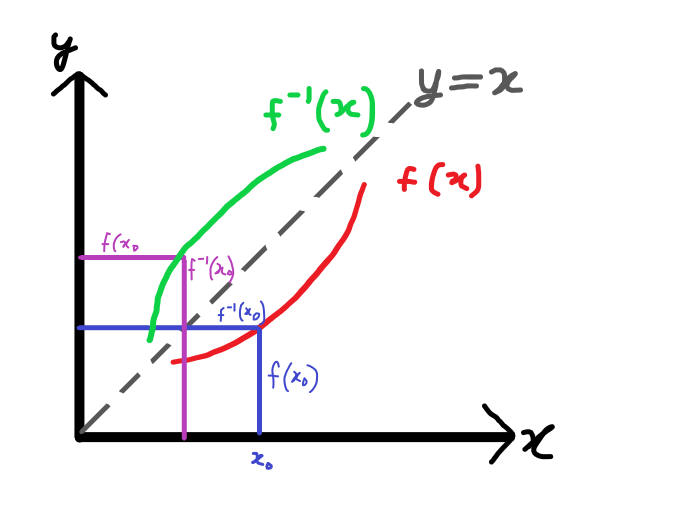
\includegraphics[scale=0.4]{images/newton_prop_1}
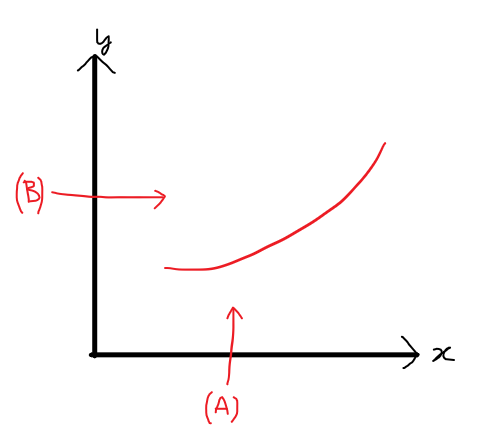
\includegraphics[scale=0.4]{images/newton_prop_2}
\end{figure}\\
So, if we look from {\color{red} (A)}, it's $f(x)$ and if we look from {\color{red} (B)}, it's $f^{-1}(x)$.\\
Now, looking at Newton's Proposition.
\[\int \limits_a^b f^{-1} = b \cdot f^{-1}(b) - a \cdot f^{-1}(a) - \int\limits_{f^{-1}(a)}^{f^{-1}(b)} f \]
\[\Leftrightarrow \int \limits_a^b f^{-1} + \int\limits_{f^{-1}(a)}^{f^{-1}(b)} f = b \cdot f^{-1}(b) - a \cdot f^{-1} (a)\]
\[\Leftrightarrow \text{Area of region {\color{blue}(i)}} + \text{Area of region {\color{purple}(ii)}} = \text{Area of rectangle OABC} - \text{Area of rectangle ODEF}\]\\
\begin{figure}[h]
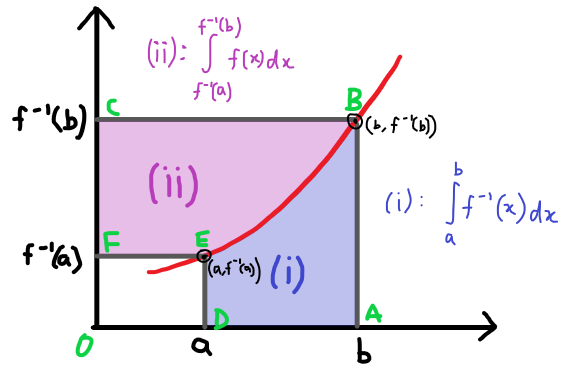
\includegraphics[scale=0.73]{images/newton_prop_3}
\end{figure}
\pagebreak
\subsection{Young's Inequality}
Suppose that $f$ is a continuous increasing function with $f(0) = 0$. Then for $a, b > 0$,
\[\int\limits_0^a f(x) \dif x + \int\limits_0^b f^{-1}(x) \dif x  \geq ab\]
and the equality holds iff $a = f^{-1}(b)$
\subsubsection{Formal Proof}
\textbf{Note:} In such theoretical proofs, one nice way of substitution can be such that the limits of integration can be made equal to those of the integral on the RHS, just like we did for proving Newton's Proposition.\\
\begin{proof}
\begin{align*}
I &= \int\limits_0^a f(x) \dif x + \int\limits_0^b f^{-1}(x) \dif x  && \text{Using Newton's Proposition}\\
&= \int\limits_0^a f(x) \dif x + b \cdot f^{-1}(b) - \int\limits_0^{f^{-1}(b)}f(x) \dif x && \text{Using } \int\limits_a^b f = - \int\limits_b^a f\\
&= \int\limits_{f^{-1}(b)}^0 f(x) \dif x + \int\limits_0^a f(x) \dif x + b \cdot f^{-1}(b) && \text{Using } \int\limits_a^c f + \int\limits_c^b f = \int\limits_a^b f\\
&= \int\limits_{f^{-1}(b)}^a f(x) \dif x + b \cdot f^{-1}(b) && \text{Add and subtract } ab\\
&= \int\limits_{f^{-1}(b)}^a f(x) \dif x + b \cdot f^{-1}(b) - ab + ab && \text{Factor out } b
\end{align*}
$\left[ \text{Wishful thinking: if we can prove }\displaystyle\int\limits_{f^{-1}(b)}^a f(x) \dif x + b \cdot f^{-1}(b) - ab \text{ is nonnegative, we are done.} \right]$
\begin{align*}
\Rightarrow I &= \int\limits_{f^{-1}(b)}^a f(x) \dif x + b \cdot \left( f^{-1}(b) - a\right) + ab && \text{Express } f^{-1}(b) - a = \int\limits_a^{f^{-1}(b)}1\dif x\\
&= \int\limits_{f^{-1}(b)}^a f(x) \dif x + b \int\limits_a^{f^{-1}(b)}\dif x + ab && \text{Using } \int\limits_a^b f = - \int\limits_b^a f \text{ and } k \int\limits_a^b f = \int\limits_a^b kf\\
&= \int\limits_{f^{-1}(b)}^a f(x) \dif x - \int\limits_{f^{-1}(b)}^a b \dif x + ab && \text{Using } \int\limits_a^b f + \int\limits_a^b g = \int\limits_a^b (f+g)\\
&= \int\limits_{f^{-1}(b)}^a \left(f(x) - b\right) \dif x + ab
\end{align*}
We have
$I = \displaystyle\int\limits_{f^{-1}(b)}^a \left(f(x) - b\right) \dif x + ab$.\\
Three cases arise.
\begin{case} {If $a = f^{-1}(b)$}\\
\begin{align*}
I &= \int\limits_a^a \left(f(x) - b\right) \dif x + ab && \text{Using } \int\limits_a^a f = 0\\
&= 0 + ab\\
&= ab \geq ab
\end{align*}
This proves that equality holds if $a = f^{-1}(b)$
\end{case}
\begin{case}
If $a > f^{-1}(b)$
\[I = \displaystyle\int\limits_{f^{-1}(b)}^a \left(f(x) - b\right) \dif x + ab\]
\[\Rightarrow f^{-1}(b) \leq x \leq a\]
Since $f$ is a strictly increasing function, we can compose this with $f$.
\[\Rightarrow f\left( f^{-1}(b) \right) \leq f(x) \leq f(a)\]
\[\Rightarrow b \leq f(x) \leq f(a)\]
So $f(x) \geq b$\\
Therefore $f(x) - b \geq 0$\\
And since $a > f^{-1}(b)$,
\[\int\limits_{f^{-1}(b)}^a \left( f(x) - b \right) > 0\]
\[\Rightarrow \int\limits_{f^{-1}(b)}^a \left( f(x) - b \right) + ab > ab\]
\end{case}
\begin{case}
If $a < f^{-1}(b)$
\[I = \displaystyle\int\limits_{f^{-1}(b)}^a \left(f(x) - b\right) \dif x + ab = \int\limits_a^{f^{-1}(b)} \left(b - f(x)\right) \dif x + ab\]
\[\Rightarrow a \leq x \leq f^{-1}(b) \Rightarrow f(a) \leq f(x) \leq b\]
Therefore $b - f(x) \geq 0$\\
And since $f^{-1(b)} > a$,
\[\int\limits_a^{f^{-1}(b)} \left(b - f(x)\right) \dif x > 0\]
\[\Rightarrow \int\limits_a^{f^{-1}(b)} \left(b - f(x)\right) \dif x + ab > ab\]
\end{case}
\end{proof}
\pagebreak
\subsubsection{Graphical Intuition}
$f$ is a strictly increasing function and $f(0) = 0$.
\begin{figure}[h]
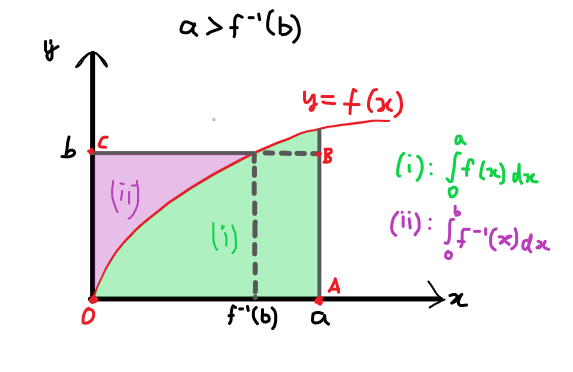
\includegraphics[scale=.55]{images/youngs_inequality_1}
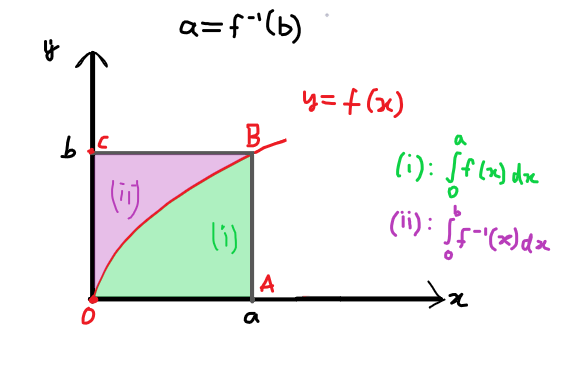
\includegraphics[scale=.55]{images/youngs_inequality_2}
\end{figure}
\begin{figure}[h]
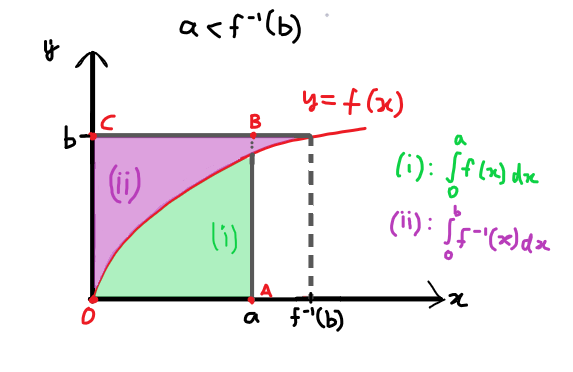
\includegraphics[scale=.55]{images/youngs_inequality_3}
\end{figure}\\
In all of the cases,\\
\[\text{Area of region {\color{green}(i)}} + \text{Area of region {\color{purple}(ii)}} \geq \text{Area of rectangle } {\color{red}OABC}\]
\[\Rightarrow {\color{green}\int\limits_0^a f(x) \dif x} + {\color{purple} \int\limits_0^b f^{-1}(x) \dif x} \geq ab\]
\[\int\limits_0^a f(x) \dif x + \int\limits_0^b f^{-1}(x) \dif x \geq ab\]
\begin{flushright}
\qedsymbol
\end{flushright}
\pagebreak
\subsection{Problems}
\begin{prob}
$\displaystyle \int\limits_1^5 (x-1)(x-2)(x-3)(x-4)(x-5) \dif x$
\begin{align*}
I &= \int\limits_1^5 (x-1)(x-2)(x-3)(x-4)(x-5) \dif x && \text{Using } \int\limits_a^bf(x)\dif x = \int\limits_a^b f(a+b-x) \dif x\\
&= \int\limits_1^5 (6-x-1)(6-x-2)(6-x-3)(6-x-4)(6-x-5) \dif x\\
&= \int\limits_1^5 (5-x)(4-x)(3-x)(2-x)(1-x) \dif x\\
&= -\int\limits_1^5 (x-1)(x-2)(x-3)(x-4)(x-5) \dif x\\
&= -I
\end{align*}
\[I = - I\]
\[\Rightarrow I = 0\]
\end{prob}
\begin{prob}
$\displaystyle\int\limits_{\sqrt{\ln(2)}}^{\sqrt{\ln(3)}}\dfrac{x \sin\left( x^2 \right)}{\sin\left(x^2\right) + \sin\left(\ln(6) - x^2 \right)} \dif x$
\[I = \int\limits_{\sqrt{\ln(2)}}^{\sqrt{\ln(3)}}\dfrac{x \sin\left( x^2 \right)}{\sin\left(x^2\right) + \sin\left(\ln(6) - x^2 \right)} \dif x\]
Substitute $x^2 = t \Rightarrow 2x \dif x = \dif t$\\
$x = \sqrt{\ln(2)} \Rightarrow t = \ln(2)$ and $x = \sqrt{\ln(3)} \Rightarrow t = \ln(3)$
\begin{equation}\label{ln_integral_1}
\Rightarrow I =\dfrac12 \int\limits_{\ln(2)}^{\ln(3)} \dfrac{\sin(t)}{\sin(t) + \sin\left(\ln(6) - t \right)} \dif t
\end{equation}
Using $\displaystyle\int\limits_a^b f(x)\dif x = \int\limits_a^b f(a+b-x) \dif x$
\begin{equation}\label{ln_integral_2}
\Rightarrow I =\dfrac12 \int\limits_{\ln(2)}^{\ln(3)} \dfrac{\sin(\ln(6) - t)}{\sin(\ln(6) - t) + \sin\left(t \right)} \dif t
\end{equation}
Add \eqref{ln_integral_1} and \eqref{ln_integral_2},
\[2I = \dfrac12 \int\limits_{\ln(2)}^{\ln(3)} \dfrac{\cancel{\sin(t) + \sin\left(\ln(6) - t\right)}}{\cancel{\sin(t) + \sin\left(\ln(6) - t\right)}} \dif t = \dfrac12\left( \ln(3) - \ln(2) \right)\]
\[\Rightarrow I = \dfrac14 \left(\ln(3) - \ln(2)\right) = \dfrac14 \ln\left(\dfrac32 \right)\]
\end{prob}
\pagebreak
\begin{prob}
$\displaystyle\int\limits_0^{\dfrac{\pi}{2}} \dfrac{\sqrt{\sin(x)}}{\sqrt{\sin(x)} + \sqrt{\cos(x)}} \dif x$
\begin{equation}
I = \int\limits_0^{\dfrac{\pi}{2}} \dfrac{\sqrt{\sin(x)}}{\sqrt{\sin(x)} + \sqrt{\cos(x)}} \dif x
\end{equation}
Using property $\displaystyle \int\limits_0^a f(x) \dif x = \displaystyle \int\limits_0^a f(a-x) \dif x$
\[I = \bigint\limits_0^{\dfrac{\pi}{2}}\dfrac{\sqrt{\sin\left(\dfrac{\pi}2 - x\right)}}{\sqrt{\sin\left(\dfrac{\pi}2 - x\right)} + \sqrt{\cos\left(\dfrac{\pi}2 - x\right)}} \dif x\]
\begin{equation}
\Rightarrow I = \int\limits_0^{\dfrac{\pi}{2}}\dfrac{\sqrt{\cos(x)}}{\sqrt{\cos(x)} + \sqrt{\sin(x)}} \dif x
\end{equation}
Add equations (1) and (2)\\
\[2I = \int\limits_0^{\dfrac{\pi}{2}} \dfrac{\sqrt{\sin(x)}}{\sqrt{\cos(x)} + \sqrt{\sin(x)}} \dif x + \int\limits_0^{\dfrac{\pi}{2}}\dfrac{\sqrt{\cos(x)}}{\sqrt{\cos(x)} + \sqrt{\sin(x)}} \dif x\]
We can combine the integrals here.
\[\Rightarrow 2I = \int\limits_0^{\dfrac{\pi}{2}} \dfrac{\cancel{\sqrt{\cos(x)} + \sqrt{\sin(x)}}}{\cancel{\sqrt{\cos(x)} + \sqrt{\sin(x)}}} \dif x\]
\[\Rightarrow 2I = \dfrac{\pi}{2}\]
\[\Rightarrow I = \dfrac{\pi}{4}\]
\end{prob}
\pagebreak
\begin{prob}
Let $A = \displaystyle\int\limits_0^1 \dfrac{e^t}{t + 1} \dif t$\\
Then, express the following in terms of A.\\
(i) $I_1 = \displaystyle\int\limits_0^1 \dfrac{t\cdot {\rm e}^{t^2}}{t^2 + 1} \dif t$\\
Let $x = t^2 \quad \Rightarrow \dif x = 2t \dif t$\\
\[\Rightarrow \displaystyle\int\limits_0^1 \dfrac{t\cdot {\rm e}^{t^2}}{t^2 + 1} \dif t = \dfrac12 \int\limits_0^1 \dfrac{{\rm e}^x}{x + 1} \dif x = \dfrac12 \int\limits_0^1 \dfrac{e^t}{t + 1} \dif t = \dfrac12 (A) = \dfrac{A}2\]\\\\
(ii) $I_2 = \displaystyle\int\limits_{a-1}^a \dfrac{{\rm e}^{-t}}{t-a-1} \dif t$\\
Let $u = t - a + 1 \quad \Rightarrow \dif u = \dif t$\\
$\Rightarrow t = u + a - 1$
\[\Rightarrow \int\limits_{a-1}^a \dfrac{{\rm e}^{-t}}{t-a-1} \dif t = \int\limits_0^1 \dfrac{{\rm e}^{-u-a+1}}{u+\cancel{a}-1-\cancel{a}-1} \dif u = \int\limits_0^1 \dfrac{{\rm e}^{-u-a+1}}{u-2} \dif u \]
Using $\displaystyle \int\limits_0^a f(x) \dif x = \int\limits_0^a f(a-x) \dif x$
\[\Rightarrow I_2 = \int\limits_0^1 \dfrac{{\rm e}^{u-\cancel{1}-a+\cancel{1}}}{1-u-2} = \int\limits_0^1 \dfrac{{\rm e}^{u-a}}{-u-1} \dif u = -{\rm e}^{-a} \int\limits_0^1 \dfrac{{\rm e}^{u}}{u + 1} \dif u= -{\rm e}^{-a} \int\limits_0^1 \dfrac{{\rm e}^{t}}{t + 1} \dif t = -{\rm e}^{-a} \cdot (A)\]\\\\
(iii) $I_3 = \displaystyle \int\limits_0^1 \dfrac{{\rm e}^t}{(t+1)^2} \dif t$\\
Integrating by parts.\\
Let $u = {\rm e}^t$ and $\dif v = \dfrac{\dif t}{(t+1)^2}$\\
$\Rightarrow \dif u = {\rm e}^t \dif t$ and $v = \dfrac{-1}{t+1}$\\
$\int u \dif v = uv - \int v \dif u$
\[I_3 = \left[\dfrac{-{\rm e}^t}{t+1}\right]_0^1 - \int\limits_0^1 \dfrac{-{\rm e}^t}{t+1} \dif t = \dfrac{- {\rm e}}{2}  - (-1)  + \int\limits_0^1 \dfrac{{\rm e}^t}{t+1} \dif t = 1 - \dfrac{\rm e}{2} + A\]
\end{prob}
\pagebreak
\begin{prob}
Let $f(x) = \displaystyle \int\limits_1^x \dfrac{\ln(t)}{t+1} \dif t$. If $x > 0$, compute $f(x) + f\left( \dfrac1{x} \right)$  . Hence or otherwise, show that $f(2) + f\left(\dfrac12\right) = \dfrac12 \left( \ln(2) \right)^2$.\\
\textbf{Solution:}\\
\begin{align*}
f(x) &= \int\limits_1^x \dfrac{\ln(t)}{t+1} \dif t = \int\limits_1^x \dfrac{\ln(u)}{u+1} \dif u\\
f\left( \dfrac1x \right) &= \int\limits_1^{1/x} \dfrac{\ln(t)}{t+1} \dif t && \parbox[t]{5cm}{Let $t = \dfrac1u \quad \Rightarrow \dif t = \dfrac{-1}{u^2} \dif u$\\\\
$t = 1 \Rightarrow u = 1$\\\\
$t = \dfrac1x \Rightarrow u = x$}\\\\
&= \bigint\limits_1^x \dfrac{-\ln\left( \dfrac1u \right)}{\dfrac1u + 1}\left(\dfrac{\dif u}{u^2}\right)\\
&= \int\limits_1^x \dfrac{\ln(u)}{u(u+1)} \dif u\\
\text{Now, } f(x) + f\left(\dfrac1{x}\right) &= \int\limits_1^x \left[\dfrac{\ln(u)}{u+1} + \dfrac{\ln(u)}{u(u+1)} \right] \dif u\\
&= \int\limits_1^x \dfrac{u \ln(u) + \ln(u)}{u(u+1)} \dif u\\
&= \int\limits_1^x \dfrac{\ln(u) \cdot \cancel{\left( u + 1 \right)}}{u\cancel{(u+1)}} \dif u && \text{Let } v = \ln(u)\quad \Rightarrow \dfrac1u \dif u = \dif v\\
&= \int\limits_0^{\ln(x)} v \dif v = \left[ \dfrac{v^2}2 \right]_0^{\ln(x)}\\
&=  \dfrac12 \left(\ln(x)\right)^2\\
\therefore f(2) + f\left( \dfrac12 \right) &= \dfrac12 \left(\ln(2) \right)^2
\end{align*}
\begin{flushright}
\qedsymbol
\end{flushright}
\end{prob}
\pagebreak
\begin{prob}
A function $F$ is defined by the following definite integral.
\[F(x) = \int\limits_1^x \dfrac{{\rm e}^t}{t} \dif t\]
Prove that $\displaystyle\int\limits_1^x \dfrac{{\rm e}^t}{t+a} \dif t = {\rm e}^{-a} \left[ F(x+a) - F(1+a) \right]$.\\
\begin{proof}
\begin{align*}
I &= \int\limits_1^x \dfrac{{\rm e}^t}{t+a} \dif t && \parbox[t]{3cm}{
	Let $t+a = u$\\
	$\Rightarrow \dif t = \dif u$\\
	$t = 1 \Rightarrow u = 1 + a$\\
	$t = x \Rightarrow u = x + a$
}\\
&= \int\limits_{1+a}^{x+a} \dfrac{{\rm e}^{u-a}}{u} \dif u\\
&= {\rm e}^{-a}\int\limits_{1+a}^{x+a} \dfrac{{\rm e}^{u}}{u} \dif u && \text{Using } \int\limits_a^c f + \int\limits_c^b f = \int\limits_a^b f\\ 
&= {\rm e}^{-a} \left[\int\limits_{1+a}^1 \dfrac{{\rm e}^{u}}{u} \dif u + \int\limits_1^{x+a} \dfrac{{\rm e}^{u}}{u} \dif u \right] && \text{Using } \int\limits_a^b f = - \int\limits_b^a f\\
&= {\rm e}^{-a} \left[-\int\limits_1^{1+a} \dfrac{{\rm e}^{u}}{u} \dif u + \int\limits_1^{x+a} \dfrac{{\rm e}^{u}}{u} \dif u \right]\\
&= {\rm e}^{-a} \left[ \int\limits_1^{x+a} \dfrac{{\rm e}^{u}}{u} \dif u -\int\limits_1^{1+a} \dfrac{{\rm e}^{u}}{u} \dif u \right]\\
&= {\rm e}^{-a} \left[F(x+a) - F(1+a) \right]
\end{align*}
\end{proof}
\end{prob}
\pagebreak
\begin{prob}
Find a continuous function $f$ such that
\[\left[ f(x) \right]^2 = \int\limits_0^x \dfrac{f(t) \cdot \sin(t)}{2 + \cos(t)} \dif t\]
\textbf{Solution:}\\
\begin{align*}
\left[ f(x) \right]^2 &= \int\limits_0^x \dfrac{f(t) \cdot \sin(t)}{2 + \cos(t)} \dif t && \text{Differentiate both sides}\\
\Rightarrow 2\cancel{f(x)} \cdot f'(x) &= \dfrac{\cancel{f(x)} \cdot \sin(x)}{2 + \cos(x)} && \text{Divide by } 2\\
\Rightarrow f'(x) &= \dfrac12 \cdot \dfrac{\sin(x)}{2+\cos(x)}\\\\
f(x) &= \int f'(x) \dif x\\
&= \dfrac12 \int\dfrac{\sin(x)}{2+\cos(x)} \dif x && \parbox[t]{3cm}{Let $\cos(x) = t$\\
$\Rightarrow -\sin(x) \dif x = \dif t$}\\
&= -\dfrac12 \int\dfrac{\dif t}{2+t}\\
&= -\dfrac12 \ln\left(\;\abs{2+t}\right) + c\\
&= -\dfrac12 \ln\left(\;\abs{2+\cos(x)}\right) + c && c \text{ is an arbitrary constant}
\end{align*}
One such function is $f(x) = -\dfrac12 \ln\left(\;\abs{2+\cos(x)}\right)$
\end{prob}
\pagebreak
\begin{prob}
Prove that for any integral with finite limits $a$ and $b$, one can always choose a linear substitution $x = pt + q$, (where $p$ and $q$ are constants) so as to transform the integral into a new one with limits from $0$ to $1$.
\begin{proof}\text{ }\\
Let us consider any such integral $I = \displaystyle\int\limits_a^b f(x) \dif x$\\
Let $x = pt + q$\\
$\Rightarrow \dif x = p \dif t$\\
Now,
\[x = a \text{ at } t = 0\]
\[\Rightarrow pt+q = a \text{ at } t = 0\]
\[\therefore q = a\]
And,
\[x = b \text{ at } t = 1\]
\[\Rightarrow pt+q = b \text{ at } t = 1\]
\[\Rightarrow p + q = b\]
\[\Rightarrow p = b - a\]
So,
\[\int\limits_a^b f(x) \dif x = p \int\limits_0^1 f(pt+q) \dif t\]
where $p = b - a$ and $q = a$.\\
So for any integral with finite limits $a$ to $b$, we can substitute $x = (b-a)t + a$ to change the limits to $0$ to $1$.
\[\int\limits_a^b f(x) \dif x = (b-a) \cdot \int\limits_0^1 f\left((b-a)t + a\right) \dif t\]
\end{proof}\text{}\\
\textbf{Problem-Solving Tip: } In a general problem involving addition of two integrals, try to convert both of them into an integral of the form $\displaystyle\int\limits_0^1$ and then add.
\end{prob}
\pagebreak
\begin{prob}
$\displaystyle\int\limits_{-4}^{-5} {\rm e}^{(x+5)^2} \dif x + 3\int\limits_{1/3}^{2/3} {\rm e}^{9\left(x - \frac23\right)^2}\dif x$\\\\
Let $p(x) = {\rm e}^{(x+5)^2}$ and $q(x) = {\rm e}^{9\left(x - \frac23\right)^2}$
\begin{align*}
I &= \int\limits_{-4}^{-5} {\rm e}^{(x+5)^2} \dif x + 3\int\limits_{1/3}^{2/3} {\rm e}^{9\left(x - \frac23\right)^2}\dif x\\
&= \int\limits_{-4}^{-5} p(x) \dif x + 3\int\limits_{1/3}^{2/3} q(x) \dif x && \text{Using } \displaystyle\int\limits_a^b f(x) \dif x = (b-a) \int\limits_0^1 f\left( (b-a)t + a \right)\dif t\\
&= \int\limits_0^1 p(-t-4) \dif t + \int\limits_0^1 q\left( \dfrac13 t + \dfrac13 \right) \dif t\\
&= -1\int\limits_0^1 {\rm e}^{\left( (-t-4) + 5 \right)^2} \dif t + 3 \left( \dfrac13 \right) \int\limits_0^1 {\rm e}^{9\left(\frac13 t + \frac13 - \frac23\right)^2}\dif t\\
&= -\int\limits_0^1 {\rm e}^{\left( 1-t \right)^2} \dif t +  \int\limits_0^1 {\rm e}^{9\left(\frac{t-1}{3} \right)^2}\dif t\\
&= -\int\limits_0^1 {\rm e}^{\left( 1-t \right)^2} \dif t + \int\limits_0^1 {\rm e}^{\left( t-1 \right)^2}\dif t\\
&= \cancel{-\int\limits_0^1 {\rm e}^{\left( t-1 \right)^2} \dif t} +  \cancel{\int\limits_0^1 {\rm e}^{\left( t-1 \right)^2}\dif t}\\
&= 0
\end{align*}
\end{prob}
\begin{prob}
Let $f: \mathbb{R} \to \mathbb{R}$ and $g:\mathbb{R} \to \mathbb{R}$ be continuous functions. Then find the value of
\[ I = \int\limits_{-\pi/2}^{\pi/2} \left[ f(x) + f(-x) \right] \cdot \left[ g(x) - g(-x) \right] \dif x \]
Let $h(x) = \left[ f(x) + f(-x) \right] \cdot \left[ g(x) - g(-x) \right]$\\
\begin{align*}
h(x) &= \left[ f(x) + f(-x) \right] \cdot \left[ g(x) - g(-x) \right]\\
\Rightarrow h(-x) &= \left[ f(-x) + f(x) \right] \cdot \left[ g(-x) - g(x) \right]\\
&= \left[ f(-x) + f(x) \right] \cdot (-1) \left[ g(x) - g(-x) \right]\\
&= -h(x)
\end{align*}
$\Rightarrow h(x)$ is an odd function.\\
We know that $\displaystyle\int_{-a}^a f = 0$ if $f(-x) = -f(x)$\\\
$\therefore I = 0$\\
And we're done.
\end{prob}
\pagebreak
\paragraph{Remark:} It is often a good idea to shift the origin to the midpoint of the limits of integration, thereby making them of the form $\int\limits_{-a}^a$.
\begin{prob}
$\displaystyle \int\limits_{-2}^0 \left( x^3 + 3x^2 + 3x + 3 + (x+1)\cos(x+1) \right) \dif x$\\
\begin{align*}
I &= \int\limits_{-2}^0 \left( x^3 + 3x^2 + 3x + 3 + (x+1)\cdot\cos(x+1) \right) \dif x\\
&= \int\limits_{-2}^0 \left( (x+1)^3 + 2 + (x+1)\cdot \cos(x+1) \right) \dif x
\end{align*}
Let us shift the origin this time.\\
Let $x + 1 = t$\\
$\Rightarrow \dif x = \dif t$
\begin{align*}
\Rightarrow I &= \int\limits_{-1}^1 \left( t^3 + 2 + t \cos(t) \right) \dif t && \text{Note that } t^3 + t\cos(t) \text{ is an odd function}\\
&= \int\limits_{-1}^1 2 \dif t\\
&= \left[ 2x \right]_{-1}^1\\
&= 4
\end{align*}
\end{prob}
\begin{prob}
$\displaystyle\int\limits_0^1 \sqrt[3]{2x^3 - 3x^2 - x + 1} \dif x \quad\quad$ [Putnam]
\[I = \int\limits_0^1 \sqrt[3]{2x^3 - 3x^2 - x + 1} \dif x\]
Shifting origin again,\\
Let $x - \dfrac12 = t$\\
$\Rightarrow \dif x = \dif t$
\begin{align*}
\Rightarrow I &= \int\limits_{-1/2}^{1/2} \sqrt[3]{2\left( t - \dfrac12 \right)^3 - 3 \left( t - \dfrac12 \right)^2 - \left( t - \dfrac12 \right) + 1  } \dif t\\
&= \int\limits_{-1/2}^{1/2}\sqrt[3]{2t^3 - \dfrac{5t}2} \dif t && \text{This is an odd function}\\
&= 0
\end{align*}
\end{prob}
\pagebreak
\begin{prob}
$\displaystyle \int\limits_{1/2014}^{2014} \dfrac{\tan^{-1}(x)}{x}\dif x$
\begin{equation}\label{p114eq1}
I = \int\limits_{1/2014}^{2014} \dfrac{\tan^{-1}(x)}{x}\dif x
\end{equation}
Let $x = \dfrac1t$\\
$\Rightarrow \dif x = \dfrac{-1}{t^2} \dif t$
\begin{align*}
\Rightarrow I &= \bigints\limits_{2014}^{1/2014} \dfrac{\tan^{-1} \left( \dfrac1t \right)}{\dfrac1t} \cdot \left( \dfrac{-\dif t}{t^2} \right)\\
&= -\bigints\limits_{2014}^{1/2014} \dfrac{\tan^{-1}\left( \dfrac1t \right)}{t} \dif t
\end{align*}
\begin{equation}\label{p114eq2}
\Rightarrow I = \bigints\limits_{1/2014}^{2014} \dfrac{\tan^{-1}\left( \dfrac1x \right)}{x} \dif x
\end{equation}
Adding \eqref{p114eq1} and \eqref{p114eq2},
\begin{align*}
2I &= \bigints\limits_{1/2014}^{2014} \dfrac{\tan^{-1}(x) +\tan^{-1}\left( \dfrac1x \right)}{x} && \text{Using } \tan^{-1}(x) + \tan^{-1}\left( \dfrac1x \right) = \dfrac{\pi}{2}\\
&= \dfrac{\pi}{2} \left[\ln(x)\right]_{1/2014}^{2014}\\
&= \pi \ln(2014)\\
\Rightarrow I &= \dfrac{\pi}2 \ln(2014)
\end{align*}
\end{prob}
\pagebreak
\begin{prob}
Let $f$ be a differentiable function such that $f\left( f(x) \right) = x \; \forall x \in [0, 1]$. Suppose $f(0) = 1$. Determine the value of the following integral:
\[\int\limits_0^1 \left( x - f(x) \right)^{2016} \dif x\]
\textbf{Solution:}\\
\[f\left(f(x)\right) = x \; \forall x \in [0, 1]\]
\[\Rightarrow f\left(f(0)\right) = 0\]
\[\Rightarrow f(1) = 0\]
Since $f$ is given as a differentiable function, we are allowed to differentiate it.
\[f\left(f(x)\right) = x\]
\[\Rightarrow f'\left(f(x)\right) \cdot f'(x) = 1\]
So, $f'(x)$ can never be zero.\\
By Darboux's Theorem, $f'$ has intermediate value property.\\
$\Rightarrow f'$ must preserve its sign.\\
$\Rightarrow f'(x) > 0 \; \forall x$ or $f'(x) < 0 \; \forall x$\\
But $f(0) = 1$ and $f(1) = 0$, is inconsistent with the condition that $f'(x) > 0 \; \forall x$\\
$\Rightarrow f'(x) < 0 \; \forall x$\\
$\Rightarrow f$ is strictly decreasing.\\
$\Rightarrow f : [0, 1] \to [0, 1]$ is one-one and onto, implying $f$ is invertible. 
\begin{equation} \label{p115e1}
I = \int\limits_0^1 \left( x - f(x) \right)^{2016} \dif x = \int\limits_0^1 \left( t - f(t) \right)^{2016} \dif t
\end{equation}
Substitute $x = f(t)$. This is allowed because $f$ is one-one.\\
$\Rightarrow \dif x = f'(t) \dif t$\\
$x = 0 \Rightarrow t = 1$ and $x = 1 \Rightarrow t = 0$
\begin{align*}
\Rightarrow I &= \int\limits_1^0 \left( f(t) - f\left( f(t) \right) \right)^{2016} \cdot f'(t) \dif t\\
&= -\int\limits_0^1 \left( f(t) - t \right)^{2016} \cdot f'(t) \dif t\\
\end{align*}
\begin{equation}\label{p115e2}
\Rightarrow I = -\int\limits_0^1 \left( t - f(t) \right)^{2016} \cdot f'(t) \dif t
\end{equation}
Add \eqref{p115e1} and \eqref{p115e2},
\[2I = \int\limits_0^1 \left( t - f(t)\right)^{2016} \cdot \left(1 - f'(t)\right) \dif t\]
\pagebreak
\[2I = \int\limits_0^1 \left( t - f(t)\right)^{2016} \cdot \left(1 - f'(t)\right) \dif t\]
Let $t - f(t) = u$\\
$\Rightarrow \left(1 - f'(t)\right) \dif t = \dif u$\\\\
At $t = 0$,\\ 
$u = t - f(t)\\ = 0 - f(0)\\ = 0 - 1\\ = -1$\\\\
At $t = 1$,\\
$u = t - f(t)\\ = 1 - f(1)\\ = 1 - 0 \\= 1$
\begin{align*}
\Rightarrow 2I &= \int\limits_{-1}^1 u^{2016} \dif u\\
&= \left[ \dfrac{u^{2017}}{2017} \right]_{-1}^1\\
&= \dfrac1{2017} - \dfrac{(-1)}{2017}\\
&= \dfrac2{2017}\\
\Rightarrow I &= \dfrac1{2017}
\end{align*}
\end{prob}
\begin{prob}
$\displaystyle\int\limits_{-1}^1 \dfrac{\sqrt[3]{x}}{\sqrt[3]{1 - x} + \sqrt[3]{1+x}} \dif x$
\[I = \int\limits_{-1}^1 \dfrac{\sqrt[3]{x}}{\sqrt[3]{1 - x} + \sqrt[3]{1+x}} \dif x\]
\[\text{Let } f(x) = \dfrac{\sqrt[3]{x}}{\sqrt[3]{1 - x} + \sqrt[3]{1+x}}\]
\[\Rightarrow f(-x) = \dfrac{\sqrt[3]{-x}}{\sqrt[3]{1 + x} + \sqrt[3]{1-x}} = \dfrac{-\sqrt[3]{x}}{\sqrt[3]{1 - x} + \sqrt[3]{1+x}} = -f(x)\]
$\Rightarrow f$ is an odd function.\\
\[\Rightarrow I = \int\limits_{-1}^1 f(x) \dif x = 0\]
\end{prob}
\pagebreak
\begin{prob}
Let $a$ and $b$ be positive real numbers. Evaluate:
\[\int\limits_a^b \dfrac{{\rm e}^{x/a} - {\rm e}^{b/x}}{x} \dif x\]
\textbf{Solution:}
\[I = \displaystyle\int\limits_a^b\dfrac{{\rm e}^{x/a} - {\rm e}^{b/x}}{x} \dif x\]
Let $x = \dfrac{ab}{t}$\\
$\Rightarrow \dif x = \dfrac{-ab}{t^2} \dif t$\\\\
Now, $\dfrac{x}{a} = \dfrac{\left( \dfrac{\cancel{a}b}{t} \right)}{\cancel{a}} = \dfrac{b}{t}$\\\\
$\dfrac{b}{x} = \dfrac{\cancel{b}}{\left( \dfrac{a\cancel{b}}{t} \right)} = \dfrac{t}a$
\begin{align*}
I & = \bigints\limits_b^a \dfrac{{\rm e}^{b/t} - {\rm e}^{t/a}}{\left(\dfrac{ab}{t}\right)} \cdot \dfrac{(-ab)}{t^2} \dif t\\
&= \int\limits_b^a \dfrac{{\rm e}^{t/a} - {\rm e}^{b/t}}{t} \dif t\\
&= -\int\limits_a^b \dfrac{{\rm e}^{t/a} - {\rm e}^{b/t}}{t} \dif t\\
&= -\int\limits_a^b \dfrac{{\rm e}^{x/a} - {\rm e}^{b/x}}{t} \dif x\\
&= -I\\
\Rightarrow I &= 0
\end{align*}
\end{prob}
\pagebreak
\subsection{Comparison Theorem}
\subsubsection{Statement}
\begin{theorem}
Say $f$ and $g$ are two functions such that $f(x) \geq g(x) \quad \forall x \in (a, b)$, then\\ $\displaystyle \int\limits_a^b f(x) \dif x \geq \int\limits_a^b g(x) \dif x$ and the equality holds iff $f(x) = g(x) \quad \forall x \in (a, b)$.
\end{theorem}
\subsubsection{Corollaries}
\begin{corollary}
If $f(x) \geq 0 \quad \forall x \in (a, b)$, then $\displaystyle\int\limits_a^b f(x) \geq 0$.
\end{corollary}
\begin{corollary}
If $f(x) \geq 0 \quad \forall x \in (a, b)$ and $\displaystyle\int\limits_a^b f(x) \dif x = 0$, then $f(x) = 0$.
\end{corollary}
\subsubsection{Problems}
\begin{prob}
Arrange $I_1, I_2, I_3$ and $I_4$ in decreasing order.\\
$I_1 = \displaystyle\int\limits_0^{\pi/4}{\rm e}^{x^2} \dif x$\\
$I_2 = \displaystyle\int\limits_0^{\pi/4}{\rm e}^{x} \dif x$\\
$I_3 = \displaystyle\int\limits_0^{\pi/4}{\rm e}^{x^2} \cdot \cos(x) \dif x$\\
$I_4 = \displaystyle\int\limits_0^{\pi/4}{\rm e}^{x^2} \cdot \sin(x) \dif x$\\
\textbf{Solution: } For $x \in \left(0, \dfrac{\pi}{4} \right)$, which is a subset of $(0, 1)$,
\[{\rm e}^x > {\rm e}^{x^2} > {\rm e}^{x^2} \cdot \cos(x) > {\rm e}^{x^2} \cdot \sin(x)\]
Using Comparison Theorem,
\[\Rightarrow \int\limits_0^{\pi/4} {\rm e}^x > \int\limits_0^{\pi/4} {\rm e}^{x^2} > \int\limits_0^{\pi/4} {\rm e}^{x^2} \cdot \cos(x) > \int\limits_0^{\pi/4} {\rm e}^{x^2} \cdot \sin(x)\]
\[\Rightarrow I_2 > I_1 > I_3 > I_4\]
\end{prob}
\pagebreak
\begin{prob}
Find the total number of distinct $x \in [0, 1]$ for which $\displaystyle\int\limits_0^x \dfrac{t^2}{1+t^4} \dif t = 2x-1$.\\
\textbf{Solution:}\\
\[\text{Let } f(x) = \int\limits_0^x \dfrac{t^2}{1+t^4} \dif t - 2x + 1\]
We are concerned with the number of roots of $f(x)$ in $[0, 1]$.\\
Note that $f$ is continuous in $[0, 1]$ and differentiable in $(0, 1)$. Applying Bolzano's Theorem:
\[f(0) = \int\limits_0^0 \dfrac{t^2}{1+t^4} \dif t - 0 + 1 = 1\]
\[\Rightarrow f(0) > 0\]
\[f(1) = \int\limits_0^1 \dfrac{t^2}{1+t^4} \dif t - 1\]
Now, for $t \in (0, 1)$, $t^2 < 1$ and $1 + t^4 > 1$\\
$\Rightarrow t^2 < 1 + t^4$\\
$\Rightarrow \dfrac{t^2}{1+t^4} < 1$\\
Applying Comparison Theorem,\\
$\Rightarrow \displaystyle\int\limits_0^1 \dfrac{t^2}{1+t^4} \dif t < 1$ 
\[\Rightarrow f(1) < 0\]
By Bolzano's Theorem, since $f$ is continuous, $f(0) > 0$ and $f(1) < 0$, there exists \textbf{at least one} root of $f(x)$ in $(0, 1)$.\\
Now, assume for the purpose of contradiction that $f$ has two (or more) roots in $(0, 1)$.\\
Then, by Rolle's Theorem, $f'(x)$ has at least one root in $(0, 1)$.
\[f'(x) = \dfrac{x^2}{1+x^4} -2\]
Since $\dfrac{x^2}{1+x^4} < 1 \; \forall x \in (0, 1)$, this implies $f'(x)$ can't be zero for any $x \in (0, 1)$\\
$\Rightarrow f'(x)$ has no root in $(0, 1)$. This is a contradiction.\\
$\therefore f(x)$ has exactly one root in $(0, 1)$.\\
Therefore, there exists exactly one value of $x \in [0, 1]$ such that $\displaystyle\int\limits_0^x \dfrac{t^2}{1+t^4} \dif t = 2x-1$.
\end{prob}
\pagebreak
\begin{prob}
Find all continuous functions $f:[0, 1] \to \mathbb{R}$ satisfying 
\[\int\limits_0^1 f(x) \dif x = \dfrac13 + \int\limits_0^1 \left( f\left( x^2 \right) \right)^2 \dif x\]
\textbf{Solution:}
\[\int\limits_0^1 f(x) \dif x = \dfrac13 + \int\limits_0^1 \left( f\left( x^2 \right) \right)^2 \dif x\]
Let us try to express $\dfrac13$ as an integral, it may help us simplify stuff.\\
$\dfrac13 = \displaystyle\int\limits_0^1 x^2 \dif x$
\[\Rightarrow \int\limits_0^1 f(x) \dif x = \int\limits_0^1 x^2 \dif x + \int\limits_0^1 \left( f\left( x^2 \right) \right)^2 \dif x\]
Now let us try to express the whole thing in terms of $x^2$.\\
Substitute $x = t^2$ in LHS. This is allowed because $t^2$ is one-one for $t \in (0,1)$\\
$\Rightarrow \dif x = 2t \dif t$
\[\Rightarrow \int\limits_0^1 f\left(t^2\right) \cdot 2t \dif t = \int\limits_0^1 x^2 \dif x + \int\limits_0^1 \left( f\left( x^2 \right) \right)^2 \dif x\]
\[\Rightarrow \int\limits_0^1 f\left(x^2\right) \cdot 2x \dif x = \int\limits_0^1 x^2 \dif x + \int\limits_0^1 \left( f\left( x^2 \right) \right)^2 \dif x\]
Combine the integrals, bring to one side.
\[\Rightarrow \bigintsss\limits_0^1 \left[ \left( f\left( x^2 \right) \right)^2 + x^2 - 2x \cdot f\left(x^2\right)    \right] \dif x = 0\]
\[\Rightarrow \bigintsss\limits_0^1 \left( f\left(x^2\right) - x \right)^2 \dif x = 0\]
Now, $\left( f\left(x^2\right) - x \right)^2 \geq 0 \; \forall x$ ($\because$ the square of a real number is always non-negative)\\
$\Rightarrow \displaystyle\bigintsss\limits_0^1 \left( f\left(x^2\right) - x \right)^2 \dif x \geq 0$\\
By Comparison Theorem, $\left( f\left(x^2\right) - x \right)^2 = 0$
\[\Rightarrow f\left( x^2 \right) = x\]
\[\Rightarrow f(x) = \sqrt{x}\]
Therefore, $f(x) = \sqrt{x}$ is the only continuous function that satisfies the property.
\end{prob}
\pagebreak
\begin{prob}
Determine the continuous functions $f:[0, 1] \to \mathbb{R}$ satisfying
\[ \int\limits_0^1 f(x) \cdot \left( x - f(x)\right) \dif x = \dfrac1{12} \]
\textbf{Solution:}
\[ \int\limits_0^1 f(x) \cdot \left( x - f(x)\right) \dif x = \dfrac1{12} \]
Let us try to express $\dfrac1{12}$ as an integral with limits 0 to 1.\\
\[ \Rightarrow \int\limits_0^1 \left(x \cdot f(x) - \left(f(x)\right)^2 \right) \dif x = \int\limits_0^1 \dfrac{x^2}{4} \dif x \]
\[ \Rightarrow \bigintsss\limits_0^1\left( \left(f(x)\right)^2 - x \cdot f(x) + \dfrac{x^2}{4} \right) \dif x = 0\]
\[\Rightarrow \int\limits_0^1 \left( f(x) - \dfrac{x}2 \right)^2 \dif x = 0\]
Now, $\left( f(x) - \dfrac{x}2 \right)^2 \geq 0 \; \forall x$\\
$\Rightarrow \displaystyle\int\limits_0^1 \left( f(x) - \dfrac{x}2 \right)^2 \dif x \geq 0 $\\\\
Using the comparison theorem (Corollary 2),
\[\Rightarrow f(x) - \dfrac{x}2 = 0\]
\[\Rightarrow f(x) = \dfrac{x}2\]
\end{prob}
\subsection{Average Value of a Function}
The average value of a function $f$ on an interval $[a, b]$ is defined as
\[\dfrac{\displaystyle\int\limits_a^b f(x) \dif x}{b-a}\]
The average value of a function $f$ over a function $g$ on the interval $[a, b]$ is defined as
\[\dfrac{\displaystyle\int\limits_a^b f(x)\cdot g(x) \dif x}{\displaystyle \int\limits_a^b g(x) \dif x}\]
\pagebreak
\subsection{Mean Value Theorems for Integrals}
\begin{theorem}
Say a function $f$ is continuous on $[a, b]$, then there exists $c \in (a, b)$ such that:
\[\int\limits_a^b f(x) \dif x = f(c) \cdot (b-a)\]
\end{theorem}
\begin{proof}
Since $f$ is continuous on a closed interval, $f$ will have at least one absolute minimum and at least one absolute maximum value.\\
Let $m$ and $M$ be the minimum and maximum values attained by $f$ respectively.
\[m \leq f(x) \leq M\]
Using Comparison Theorem, integrating throughout.
\[\int\limits_a^b m \dif x \leq \int\limits_a^b f(x) \dif x \leq \int\limits_a^b M \dif x\]
\[\Rightarrow m(b-a) \leq \int\limits_a^b f(x) \dif x \leq M(b-a)\]
Since $b \geq a$, we can divide by $b-a$ without changing the signs of the inequality.
\[\Rightarrow m \leq \dfrac{\displaystyle\int\limits_a^b f(x)\dif x}{b-a} \leq M\]
By Intermediate Value Theorem, $\dfrac{\displaystyle\int\limits_a^b f(x)\dif x}{b-a}$ will take all the values between its maximum $M$ and minimum $m$.
\[\exists\; c \in [a, b] : \dfrac{\displaystyle\int\limits_a^b f(x)\dif x}{b-a} = f(c)\]
\[\Rightarrow \exists\; c \in [a, b] : \int\limits_a^b f(x)\dif x = f(c) \cdot (b-a)\]
\end{proof}
\pagebreak
\subsubsection{The General Mean Value Theorems}
\begin{theorem}
Let $f$ and $g$ be two continuous functions in $[a, b]$ such that on the given interval, $g$ does not change sign. Then there exists some  $c \in [a, b]$ such that:
\[\int\limits_a^b f(x) \cdot g(x) \dif x = f(c) \cdot \int\limits_a^b g(x) \dif x\]
\end{theorem}
\begin{proof}
It is given that $g$ doesn't change sign.\\
WLOG, consider the case where $g(x) > 0$.\\
Since $f$ is continuous on a closed interval, $f$ will have at least one absolute minimum and at least one absolute maximum value.\\
Let $m$ and $M$ be the minimum and maximum values attained by $f$ respectively.
\[m \leq f(x) \leq M\]
Multiply by $g(x)$
\[m \cdot g(x) \leq f(x) \cdot g(x) \leq M \cdot g(x)\]
Again, using comparison theorem, we can integrate.
\[\int\limits_a^b m \cdot g(x) \dif x \leq \int\limits_a^b f(x) \cdot g(x) \dif x \leq \int\limits_a^b M \cdot g(x) \dif x\]
\[\Rightarrow m \cdot \int\limits_a^b  g(x) \dif x \leq \int\limits_a^b f(x) \cdot g(x) \dif x \leq M \cdot \int\limits_a^b  g(x) \dif x\]
Since $g(x) > 0$, by comparison theorem, $\displaystyle\int\limits_a^b g(x) \dif x > 0$.\\
Divide by $\displaystyle\int\limits_a^b g(x) \dif x$.
\[m \leq \dfrac{\displaystyle\int\limits_a^b f(x) \cdot g(x) \dif x}{\displaystyle\int\limits_a^b g(x) \dif x} \leq M\]
By Intermediate Value Theorem $ \dfrac{\displaystyle\int\limits_a^b f(x) \cdot g(x) \dif x}{\displaystyle\int\limits_a^b g(x) \dif x}$ will take all values between its minimum $m$ and maximum $M$.\\ $\therefore\exists\; c \in [a, b]$ such that $\displaystyle \int\limits_a^b f(x) \cdot g(x) \dif x = f(c) \cdot \int\limits_a^b g(x) \dif x$
\end{proof}
\pagebreak
\begin{theorem}
Say $f$ and $g$ are continuous functions and say the derivative of $f$ is continuous and does not change sign. Then, there exists some $c \in [a, b]$ such that:
\[\int\limits_a^b f(x) \cdot g(x) \dif x = f(a) \int\limits_a^c g(x) \dif x + f(b) \int\limits_c^b g(x) \dif x\]
\end{theorem}
\begin{proof}
\[\text{Let } G(x) = \int\limits_a^x g(t) \dif t\]
\[\Rightarrow G'(x) = g(x) - g(a)\cdot \dfrac{\dif}{\dif x}(a) = g(x)\]
\[\text{Let }I = \int\limits_a^b f(x) \cdot g(x) \dif x\]
\[\Rightarrow I = \int\limits_a^b f(x) \cdot G'(x) \dif x\]
Integrating by parts.\\
Let $u = f(x)$ and $\dif v = G'(x) \dif x$\\
Then, $\dif u = f'(x) \dif x$ and $v = G(x)$\\
$\int u \dif v = uv - \int v \dif u$
\begin{align*}
\Rightarrow I &= \left[ f(x) \cdot G(x) \right]_a^b - \int\limits_a^b f'(x) \cdot G(x) \dif x\\
&= f(b) \int\limits_a^b g(x) \dif x - f(a) \int\limits_a^a g(x) \dif x - \int\limits_a^b f'(x) \cdot G(x) \dif x && \parbox[t]{3cm}{Using the previous general mean value theorem.}\\
&= f(b) \int\limits_a^b g(x) \dif x - G(c) \int\limits_a^b f'(x) \dif x && \text{For some $c$}\\
&= f(b) \int\limits_a^b g(x) \dif x - \left(\int\limits_a^c g(x) \dif x \right)\cdot\left(f(b) - f(a) \right)\\
&= f(b) \int\limits_a^b g(x) \dif x - f(b) \int\limits_a^c g(x) \dif x + f(a) \int\limits_a^c g(x) \dif x\\
&= - f(b) \int\limits_b^c g(x) \dif x + f(a) \int\limits_a^c g(x) \dif x\\
&= f(a) \int\limits_a^c g(x) \dif x + f(b) \int\limits_c^b g(x) \dif x
\end{align*}
\end{proof}
\pagebreak
\begin{prob}
Let $f : [0, \infty) \to \mathbb{R}$ be a non-decreasing continuous function. If $0 \leq x < y < z$, show that:
\[(z-x) \int\limits_y^z f(u) \dif u \geq (z - y) \int\limits_x^z f(u) \dif u\]
\begin{proof}
Effectively, we have to prove that:
\[\dfrac{\displaystyle\int\limits_y^z f(u) \dif u}{(z - y)} \geq \dfrac{\displaystyle\int\limits_x^z f(u) \dif u}{(z - x)}\]
i.e. Fundamentally, we have to prove that the average of the function is a non-decreasing function.
\[\text{Let } g(t) = \dfrac{\displaystyle\int\limits_t^z f(u) \dif u}{(z - t)}\]
\begin{align*}
g'(t) &= \dfrac{-(z-t) \cdot f(t) - \left(\displaystyle\int\limits_t^z f(u) \dif u\right) (-1)}{(z-t)^2}\\
&= \dfrac{\displaystyle\int\limits_t^z f(u) \dif u-(z-t) \cdot f(t)}{(z-t)^2} && \parbox[t]{4.5cm}{Wishful thinking:\\ Denominator is non-negative. If we can prove the numerator is non-negative, we are done}\\
\text{Now, } \int\limits_t^z f(u) \dif u = (z-t) f(c) &\text{ } \text{for some } c \in (t, z) && \parbox[t]{4.5cm}{Using Mean Value Theorem for integrals}\\
\Rightarrow g'(t) &= \dfrac{(z-t) f(c) - (z-t) f(t)}{(z-t)^2}\\
&= \dfrac{(z-t) \left(f(c) - f(t)\right)}{(z-t)^2}
\end{align*}
Now, $c \in [t, z] \Rightarrow c > t$\\
$\Rightarrow f(c) \geq f(t)$, since $f$ is non-decreasing.\\
Also, $t \leq z$.
\[\Rightarrow g'(t) \geq 0\]
$\Rightarrow g(t)$ is non-decreasing.\\
\[\Rightarrow \dfrac{\displaystyle\int\limits_y^z f(u) \dif u}{(z - y)} \geq \dfrac{\displaystyle\int\limits_x^z f(u) \dif u}{(z - x)}\]
\[\Rightarrow (z-x) \int\limits_y^z f(u) \dif u \geq (z - y) \int\limits_x^z f(u) \dif u\]
\end{proof}
\end{prob}
\pagebreak
\begin{prob}
If $\phi''$ is continuous and non-zero on the closed interval $[a, b]$ and if there is a constant $m > 0$ such that $\phi'(t) \geq m \; \forall t \in [a, b]$, then prove that $\abs{\displaystyle\int\limits_a^b \sin\left(\phi(t)\right) \dif t} \leq \dfrac4m$
\begin{proof}
Let $I = \displaystyle\int\limits_a^b \sin\left(\phi(t)\right) \dif t$
\[\Rightarrow I = \int\limits_a^b \dfrac{\sin\left(\phi(t)\right)}{\phi'(t)} \cdot \phi'(t) \dif t\]
Let $f(t) = \dfrac1{\phi'(t)}$ and $g(t) = \sin\left(\phi(t)\right) \cdot \phi'(t)$\\
Then, 
\[I = \int\limits_a^b f(t)\cdot g(t) \dif t\]
$f'(t) = \dfrac{-\phi'(t)}{\left[ \phi''(t) \right]^2}$\\
Since $\phi''$ is continuous and non-zero, this implies $\phi''$ preserves its sign.\\
Using the Second General Mean Value Theorem, $\exists c \in [a, b]$ such that
\begin{align*}
I &= f(a) \int\limits_a^c g(t) \dif t + f(b) \int\limits_c^b g(t) \dif t\\
\Rightarrow \int\limits_a^b \dfrac{\sin\left(\phi(t)\right)}{\phi'(t)} \cdot \phi'(t) \dif t &= \dfrac1{\phi'(a)} \int\limits_a^c \sin\left(\phi(t)\right) \cdot \phi'(t) \dif t + \dfrac1{\phi'(b)} \int\limits_c^b \sin\left(\phi(t)\right) \cdot \phi'(t) \dif t
\end{align*}
Using the Triangle Inequality $\abs{x+y} \leq \abs{x} + \abs{y} \; \forall x, y \in \mathbb{C}$,
\[\Rightarrow \abs{I} \leq \abs{\dfrac1{\phi'(a)}\int\limits_a^c \sin\left(\phi(t)\right)\phi'(t) \dif t} + \abs{\dfrac1{\phi'(b)}\int\limits_c^b \sin\left(\phi(t)\right)\phi'(t) \dif t}\]%//
\[\Rightarrow \abs{I} \leq \abs{\dfrac{\left[-\cos\left(\phi(t)\right) \right]_a^c}{\phi'(a)}} + \abs{\dfrac{\left[-\cos\left(\phi(t)\right)\right]_c^b}{\phi'(b)}}\]
Now,
\[\phi'(t) \geq m \Rightarrow \dfrac1{\phi'(t)} \leq \dfrac1{m}\]
And the maximum difference of $\cos(x)$ is $2$.
\[\Rightarrow \abs{I} \leq \dfrac2m + \dfrac2m\]
\[\Rightarrow \abs{\int\limits_a^b \sin\left(\phi(t)\right) \dif t} \leq \dfrac4m\]
\end{proof}
\end{prob}
\pagebreak
\subsection{Estimation of Integrals}
\textbf{Note:} Estimates may be good or bad, but are seldom incorrect.
\subsubsection{Method - 1: Comparison Theorem}
Suppose we need to estimate $\displaystyle\int\limits_a^b f(x) \dif x$.\\
We will estimate $f(x)$ between two functions whose integrals can be evaluated.
\[g(x) < f(x) < h(x)\]
Then, we'll use comparison theorem and evaluate.\\
Also, we can use the fact that $\abs{\displaystyle\int\limits_a^b f(x) \dif x} \geq \displaystyle\int\limits_a^b \abs{f(x)} \dif x$.\\
For example, if we need to estimate $\displaystyle\int\limits_0^1 {\rm e}^{-x^2} \dif x$, then ${\rm e}^{-x^2}$ can be estimated in two ways:
\[1-x^2 \leq {\rm e}^{-x^2} \leq \dfrac1{1 - x^2} \text{\quad\quad Better, More precise}\]
\[{\rm e}^{-x} \leq {\rm e}^{-x^2} \leq 1 \text{\quad\quad Not as precise}\]
\subsubsection{Method - 2: Using a Minimum and Maximum Value}
Say $f$ is a continuous function.\\
To estimate $\displaystyle\int\limits_a^b f(x) \dif x$, we can find the minimum and maximum values of $f$. Say the minimum is $m$ and the maximum is $M$.
\[m \leq f(x) \leq M\]
Apply comparison theorem,
\[m(b-a) \leq \int\limits_a^b f(x) \dif x \leq M(b-a)\]
\subsubsection{Method - 3: Mean Value Theorem for Integrals}
\[\int\limits_a^b f(x) \dif x = f(c) \cdot (b-a), \quad \text{for some }c \in [a, b]\]
If $f$ is a non-decreasing function,\\
then $a \leq c \leq b \Rightarrow f(a) \leq f(c) \leq f(b)$
\[\Rightarrow f(a) \cdot (b-a) \leq \int\limits_a^b f(x) \dif x \leq f(b) \cdot (b-a)\]
If $f$ is a non-increasing function,\\
then $a \leq c \leq b \Rightarrow f(a) \geq f(c) \geq f(b)$
\[\Rightarrow f(a) \cdot (b-a) \geq \int\limits_a^b f(x) \dif x \geq f(b) \cdot (b-a)\]
\pagebreak
\subsubsection{Method - 4: General Mean value Theorem for Integrals}
\[\int\limits_a^b f(x) \cdot g(x) \dif x  = f(c) \cdot \int\limits_a^b g(x) \dif x, \quad \text{for some }c \in [a, b]\]
If $f$ is a non-decreasing function,\\
then $a \leq c \leq b \Rightarrow f(a) \leq f(c) \leq f(b)$
\[\Rightarrow f(a) \cdot \int\limits_a^b g(x) \dif x \leq \int\limits_a^b f(x) \cdot g(x) \dif x \leq f(b) \cdot \int\limits_a^b g(x) \dif x\]
If $f$ is a non-increasing function,\\
then $a \leq c \leq b \Rightarrow f(a) \geq f(c) \geq f(b)$
\[\Rightarrow f(a) \cdot \int\limits_a^b g(x) \dif x \geq \int\limits_a^b f(x) \cdot g(x) \dif x \geq f(b) \cdot \int\limits_a^b g(x) \dif x\]
\subsubsection{Method - 5: Cauchy-Schwarz Inequality}
If $f$ and $g$ are two functions integrable on $[a,b]$. Then,
\[\abs{\int\limits_a^b f(x) \cdot g(x) \dif x} \leq \sqrt{\int\limits_a^b \left( f(x) \right)^2 \dif x \cdot \int\limits_a^b \left( g(x) \right)^2 \dif x}\]
and equality holds iff $f(x) = \lambda \cdot g(x)$ for some constant $\lambda$.
\begin{proof}
\[\text{Let } F(x) = \left[ f(x) - \lambda \cdot g(x) \right]^2\]
Now, $F(x) \geq 0 \; \forall x \in \mathbb{R}$, because the square of a real number is always non-negative.\\
Using comparison theorem,
\[\int\limits_a^b \left( f(x) - \lambda \cdot g(x) \right)^2 \dif x \geq 0\]
\[\Rightarrow \int\limits_a^b \left(f(x) \right)^2 \dif x - 2\lambda \int\limits_a^b f(x) \cdot g(x) \dif x + \lambda^2 \int\limits_a^b \left(g(x)\right)^2 \dif x \geq 0\]
\[\Rightarrow \lambda^2 \left( \int\limits_a^b \left(g(x)\right)^2 \right) - 2\lambda \left(\int\limits_a^b f(x) \cdot g(x) \dif x \right) + \int\limits_a^b \left(f(x) \right)^2 \geq 0\]
This is a quadratic in $\lambda$. For the quadratic to be non-negative for all real $\lambda$, $D \leq 0$.
\[\Rightarrow 4 \lambda^2 \left( \int\limits_a^b f(x) \cdot g(x) \dif x \right)^2 - 4 \int\limits_a^b \left(g(x)\right)^2 \cdot \int\limits_a^b \left(f(x) \right)^2 \leq 0\]
\[\Rightarrow \abs{\int\limits_a^b f(x) \cdot g(x) \dif x} \leq \sqrt{\int\limits_a^b \left( f(x) \right)^2 \dif x \cdot \int\limits_a^b \left( g(x) \right)^2 \dif x}\]
\end{proof}
\pagebreak
\subsubsection{Method - 6: Estimation Based on Shapes}
Say $f$ is a strictly increasing function.\\
If $f$ is concave up,
\begin{figure}[h]
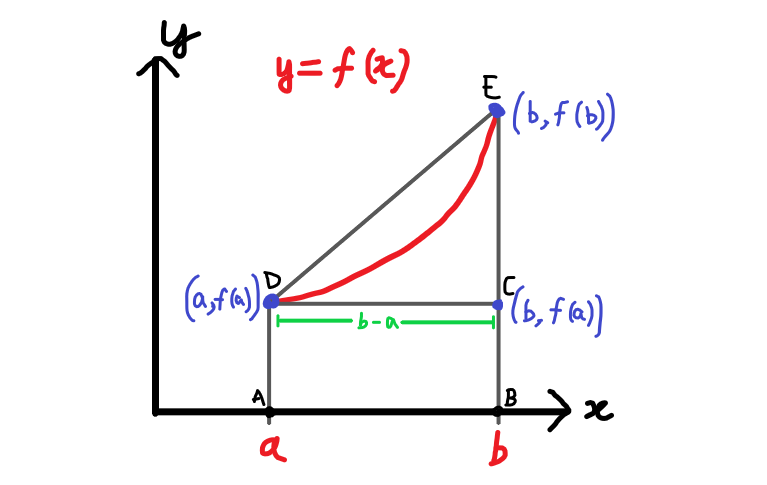
\includegraphics[scale=.5]{images/shape_estimation_1}
\end{figure}
\[\text{Area of rectangle ABCD} \leq \text{Area under curve } f \leq \text{Area of trapezium ABED}\]
\[\Rightarrow (b-a)\cdot f(a) \leq \int\limits_a^b f(x) \dif x \leq \dfrac12 \left( f(a) + f(b) \right)(b-a)\]
Similarly, if $f$ is concave down,
\begin{figure}[h]
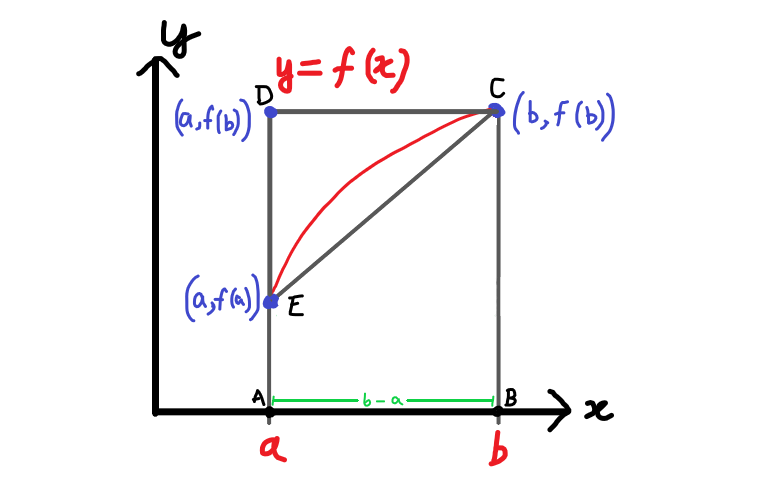
\includegraphics[scale=.5]{images/shape_estimation_2}
\end{figure}
\[\text{Area of trapezium ABCE} \leq \text{Area under curve } f \leq \text{Area of rectangle ABCD}\]
\[\dfrac12 \left( f(a) + f(b) \right)(b-a) \leq \int\limits_a^b f(x) \dif x \leq (b-a) \cdot f(b)\]
\pagebreak
\begin{prob}
Show that $0 < \displaystyle \int\limits_0^1 \dfrac{x^7}{\sqrt[3]{1+x^9}} \dif x < \dfrac18$\\
For $x \in (0, 1)$,
\[\dfrac{x^7}{\sqrt[3]{1+x^9}} > 0\]
By comparison theorem,
\[\int\limits_0^1 \dfrac{x^7}{\sqrt[3]{1+x^9}} \dif x > 0\]
Also, for $x \in (0, 1)$,
\[\Rightarrow \dfrac{x^7}{\sqrt[3]{1 + x^9}} < \dfrac{x^7}1\]
By comparison theorem,
\[\Rightarrow \int\limits_0^1 \dfrac{x^7}{\sqrt[3]{1+x^9}} \dif x < \int\limits_0^1 x^7 \dif x\]
\[\Rightarrow \int\limits_0^1 \dfrac{x^7}{\sqrt[3]{1+x^9}} \dif x < \left[\dfrac{x^8}{8}\right]_0^1\]
\[\Rightarrow\int\limits_0^1 \dfrac{x^7}{\sqrt[3]{1+x^9}} \dif x < \dfrac18\]
Therefore,
\[0 < \int\limits_0^1 \dfrac{x^7}{\sqrt[3]{1+x^9}} \dif x < \dfrac18\]
\end{prob}
\begin{prob}
Show that $0 < \displaystyle\int\limits_0^1 {\rm e}^{x^2} \dif x < {\rm e}$\\
For $x \in (0, 1)$,
\[x^2 < x\]
Since $\exp(x)$ is an increasing function,
\[0 < {\rm e}^{x^2} < {\rm e}^x\]
Apply comparison theorem,
\[\int\limits_0^1 0\dif x < \int\limits_0^1{\rm e}^{x^2} \dif x < \int\limits_0^1{\rm e}^x \dif x\]
\[\Rightarrow 0 < \int\limits_0^1 {\rm e}^{x^2} \dif x < \left[ {\rm e}^x \right]_0^1\]
\[\Rightarrow 0 < \int\limits_0^1 {\rm e}^{x^2} \dif x < {\rm e} - 1 < {\rm e} \]
\[\Rightarrow 0 < \int\limits_0^1 {\rm e}^{x^2} \dif x < {\rm e} \]
\end{prob}
\pagebreak
\begin{prob}
Estimate $\displaystyle\int\limits_{\pi/4}^{\pi/3} \dfrac{\sin(x)}{x} \dif x$\\
We'll approach this with multiple methods.
\paragraph{Method 1}
\[\text{Let } f(x) = \dfrac{\sin(x)}{x}\]
\begin{align*}
\Rightarrow f'(x) &= \dfrac{x\cos(x) - \sin(x)}{x^2}\\
&= \dfrac{\cos(x) \left[ x - \tan(x) \right]}{x^2}
\end{align*}
Now, for $x \in \left[\dfrac{\pi}{4}, \dfrac{\pi}{3} \right]$,
\[\cos(x) > 0, \quad x^2 > 0 \quad \text{ and } \quad \tan(x) > x\]
\[\Rightarrow f'(x) < 0\]
$\Rightarrow f(x)$ is strictly decreasing for $x\in \left[\dfrac{\pi}{4}, \dfrac{\pi}{3} \right]$.\\
Also, since $f(x)$ is continuous in $\left[\dfrac{\pi}{4}, \dfrac{\pi}{3} \right]$,
\[f\left(\dfrac{\pi}{4}\right) \geq f(x) \geq f\left( \dfrac{\pi}{3} \right)\]
So for $x \in \left(\dfrac{\pi}{4}, \dfrac{\pi}{3} \right)$,
\[\Rightarrow \dfrac{\sin\left(\dfrac{\pi}{3}\right)}{\left(\dfrac{\pi}3\right)} < \dfrac{\sin(x)}{x} <\dfrac{\sin\left(\dfrac{\pi}{4}\right)}
{\left(\dfrac{\pi}4\right)} \]
\[\Rightarrow \dfrac3{\pi} \cdot \dfrac{\sqrt{3}}{2} < \dfrac{\sin(x)}{x} < \dfrac{4}{\pi} \cdot \dfrac{1}{\sqrt{2}}\]
Using comparison theorem,
\[\int\limits_{\pi/4}^{\pi/3} \dfrac{3 \sqrt3}{2\pi} \dif x < \int\limits_{\pi/4}^{\pi/3} \dfrac{\sin(x)}{x} \dif x < \int\limits_{\pi/4}^{\pi/3} \dfrac{4}{\pi \sqrt2} \dif x \]
\[\Rightarrow \dfrac{3\sqrt3}{2\pi} \left[ \dfrac{\pi}{3} - \dfrac{\pi}{4}\right] < \int\limits_{\pi/4}^{\pi/3} \dfrac{\sin(x)}{x} \dif x < \dfrac{4}{\pi \sqrt2} \left[ \dfrac{\pi}{3} - \dfrac{\pi}{4} \right] \]
\[\Rightarrow \dfrac{\sqrt3}{8} < \int\limits_{\pi/4}^{\pi/3} \dfrac{\sin(x)}{x} \dif x < \dfrac{\sqrt2}{6}\]
\pagebreak
\paragraph{Method 2}
For $x \in \left[\dfrac{\pi}{4}, \dfrac{\pi}{3} \right]$,
\[\sin(x) < x\]
\[\Rightarrow \dfrac{\sin(x)}{x} < 1\]
By Comparison Theorem,
\[\int\limits_{\pi/4}^{\pi/3} \dfrac{\sin(x)}{x} \dif x < \int\limits_{\pi/4}^{\pi/3} 1 \dif x\]
\[\Rightarrow \int\limits_{\pi/3}^{\pi/4} \dfrac{\sin(x)}{x} \dif x < \dfrac{\pi}4 - \dfrac{\pi}3\]
\[\Rightarrow \int\limits_{\pi/4}^{\pi/3} \dfrac{\sin(x)}{x} \dif x < \dfrac{\pi}{12}\]
\paragraph{Method 3}
\[\text{Let } I = \int\limits_{\pi/4}^{\pi/3} \dfrac{\sin(x)}{x} \dif x\]
\[\Rightarrow I = \int\limits_{\pi/4}^{\pi/3} \left( \dfrac1x\right) \left(\sin(x) \right)\dif x\]
Using the General Mean Value Theorem for integrals, $\exists c \in \left(\dfrac{\pi}{4}, \dfrac{\pi}{3} \right)$ such that
\begin{align*}
I &= \dfrac1{c} \int\limits_{\pi/4}^{\pi/3} \dfrac{\sin(x)}{x} \dif x\\
&= \dfrac1c \left[ -cos(x) \right]_{\pi/4}^{\pi/3}\\
&= \dfrac1c \left[ -\cos\left( \dfrac{\pi}3 \right) + \cos\left( \dfrac{\pi}{4} \right) \right]\\
&= \dfrac1c \left[\dfrac1{\sqrt2} - \dfrac12 \right]\\
\end{align*}
Now, $\dfrac{\pi}{4} < c < \dfrac{\pi}{3}\quad \Rightarrow \dfrac{3}{\pi} < \dfrac1c < \dfrac{4}{\pi}$
\[\Rightarrow \dfrac{3}{\pi} \left[\dfrac1{\sqrt2} - \dfrac12 \right] <\int\limits_{\pi/4}^{\pi/3} \dfrac{\sin(x)}{x} \dif x < \dfrac{4}{\pi}\left[\dfrac1{\sqrt2} - \dfrac12 \right]\]
\end{prob}
\pagebreak
\begin{prob}
Show that $\dfrac1{10\sqrt{2}} \leq \displaystyle\int\limits_0^1 \dfrac{x^9}{\sqrt{1+x}} \dif x \leq \dfrac1{10}$\\
For $x \in (0, 1)$,
\[ \dfrac{x^9}{\sqrt{1+1}} \leq \dfrac{x^9}{\sqrt{1+x}} \leq \dfrac{x^9}{1}\]
Using Comparison Theorem,
\[\int\limits_0^1 \dfrac{x^9}{\sqrt2} \dif x \leq \int\limits_0^1 \dfrac{x^9}{\sqrt{1+x}} \dif x \leq \int\limits_0^1 \dfrac{x^9}{1} \dif x\]
\[\Rightarrow \dfrac1{\sqrt2} \left[ \dfrac{x^{10}}{10} \right]_0^1 \leq \int\limits_0^1 \dfrac{x^9}{\sqrt{1+x}} \dif x \leq \left[\dfrac{x^{10}}{10}\right]_0^1\]
\[\Rightarrow \dfrac1{10\sqrt2} \leq \int\limits_0^1\dfrac{x^9}{\sqrt{1+x}} \leq \dfrac1{10}\]
\end{prob}
\begin{prob}
Show that $0.692 \leq \displaystyle\int\limits_0^1 x^x \dif x \leq 1$\\
\[x^x \leq 1 \; \forall x \in (0, 1)\]
Applying Comparison Theorem
\[\int\limits_0^1 x^x \dif x \leq 1\]
Now, let $f(x) = x^x$
\[\Rightarrow f'(x) = x^x \left[ 1 + \ln(x)\right]\]
\[f'(x) = 0 \Leftrightarrow x = \dfrac1{\rm e}\]
$f(x)$ attains its minimum value at $x = \dfrac1{\rm e}$\\
So the minimum value of $f$ becomes $f\left( \dfrac1{\rm e} \right) = \left(\dfrac{1}{\rm e}\right)^{\dfrac1{\rm e}}$
\[\Rightarrow \left(\dfrac{1}{\rm e}\right)^{\dfrac1{\rm e}} \leq x^x \; \forall x \in (0, 1)\]
Using Comparison Theorem,
\[\Rightarrow \left({\dfrac1{\rm e}}\right)^{1/{\rm e}} \leq \int\limits_0^1 x^x \dif x\]
\[\Rightarrow 0.692 \leq \int\limits_0^1 x^x \dif x\]
\[\Rightarrow 0.692 \leq \int\limits_0^1 x^x \dif x \leq \dfrac1{10}\]
\end{prob}
\pagebreak
\begin{prob}
Show that $0.41 < \displaystyle\int\limits_0^1 x^{\sin(x) + \cos(x)} \dif x < 0.5$\\
We know that
\[1 < \sin(x) + \cos(x) < \sqrt2 \quad \forall x \in (0, 1)\]
\[\Rightarrow x^{\sqrt2} < x^{\sin(x) + \cos(x)} < x \quad \left[ \because x \in (0, 1) \right]\]
Using Comparison Theorem,
\[\Rightarrow \int\limits_0^1 x^{\sqrt2} \dif x < \int\limits_0^1 x^{\sin(x) + \cos(x)} \dif x < \int\limits_0^1 x \dif x\]
\[\Rightarrow \dfrac1{\sqrt2 + 1} < \int\limits_0^1 x^{\sin(x) + \cos(x)} \dif x < \dfrac12\]
\[\Rightarrow \sqrt2 - 1 < \int\limits_0^1 x^{\sin(x) + \cos(x)} \dif x < \dfrac12\]
Since $0.41 < \sqrt 2 - 1$,
\[\Rightarrow 0.41 < \int\limits_0^1 x^{\sin(x) + \cos(x)} \dif x < 0.5\]
\end{prob}
\begin{prob}
Show that $4 \leq =\displaystyle\int\limits_1^3 \sqrt{3 + x^3} \dif x \leq 2 \sqrt{30}$\\
\[\text{Let } f(x) = \sqrt{3+x^3}\]
\[f'(x) = \dfrac1{2\sqrt{3+x^2}} \cdot 3x^2\]
Since $f'(x) > 0 \; \forall x \in (1, 3)$, $f$ is strictly increasing.
\[\Rightarrow f(1) \leq f(x) \leq f(3) \quad \forall x \in (1, 3)\]
\[\Rightarrow \sqrt{3+1^2} \leq \sqrt{3+x^2} \leq \sqrt{3+3^2}\]
\[\Rightarrow 2 \leq \sqrt{3+x^2} \leq 2\sqrt3\]
Using Comparison Theorem,
\[2 \cdot (3-1) \leq \int\limits_1^3 \sqrt{3+x^2} \dif x \leq 2\sqrt3 \cdot (3-1)\]
\[\Rightarrow 4 \leq \int\limits_1^3 \sqrt{3+x^2} \dif x \leq 4\sqrt{3} < 2\sqrt{30}\]
\[\Rightarrow 4 \leq \int\limits_1^3 \sqrt{3+x^2} \dif x \leq 2\sqrt{30}\]
\end{prob}
\pagebreak
\begin{prob}
Show that $\displaystyle\int\limits_0^{\pi/2} {\rm e}^{-R \sin(x)} \dif x < \dfrac{\pi}{2R} \left(1- {\rm e}^{-R}\right)$ for $R>0$.\\
The right-hand side can be written as
\[\dfrac{\pi}{2R} \left(1- {\rm e}^{-R}\right) = \int\limits_0^{\pi/2} {\rm e}^{\frac{-2Rx}{\pi}} \dif x\]
So we have to prove:
\[\int\limits_0^{\pi/2} {\rm e}^{-R\sin(x)} \dif x < \int\limits_0^{\pi/2} {\rm e}^{\frac{-2Rx}{\pi}} \dif x\]
So, by Comparison Theorem, if we can prove
${\rm e}^{-R \sin(x)} < {\rm e}^{\frac{-2Rx}{\pi}}\quad \forall x  \in \left( 0, \dfrac{\pi}2\right)$, we're done.
\begin{proof}
Consider $f(x) = \dfrac{\sin(x)}{x}$\\
We know by differentiation that $f(x)$ is continuous and decreasing in $\left(0, \dfrac{\pi}{2} \right]$,\\ So it takes its least value at $\dfrac{\pi}2$.
\[\Rightarrow \dfrac{\sin(x)}{x} < \dfrac2{\pi}\; \forall x \in \left(0, \dfrac{\pi}{2}\right)\]
Since $x > 0$,
\[\Rightarrow \sin(x) < \dfrac{2x}{\pi}\; \forall x \in \left(0, \dfrac{\pi}{2}\right)\]
Since $R > 0$,
\[\Rightarrow -R \sin(x) > \dfrac{-2Rx}{\pi}\]
Now, since ${\rm e}^x$ is strictly increasing,
\[\Rightarrow {\rm e}^{-R \sin(x)} < {\rm e}^{\frac{-2Rx}{\pi}}\; \forall x  \in \left( 0, \dfrac{\pi}2\right)\]
Using Comparison Theorem,
\[\Rightarrow \int\limits_0^{\pi/2}{\rm e}^{-R \sin(x)}\dif x <  \int\limits_0^{\pi/2} {\rm e}^{\frac{-2Rx}{\pi}} \dif x\]
\end{proof}
\end{prob}
\pagebreak
\begin{prob}
Let $I = \displaystyle\sum\limits_{k=1}^{98} \int\limits_k^{k+1}\dfrac{k+1}{x(x+1)} \dif x$.\\
Then which of the following is/are correct?\\
\begin{enumerate*}[label=(\Alph*)]
\item $I < \dfrac{49}{50}\quad\quad
$\item $I < \ln(99)\quad\quad$
\item $I > \dfrac{49}{50}\quad\quad$
\item $I > \ln(99)\quad\quad$
\end{enumerate*}\\\\
\textbf{Solution: (B, C) }\\
For $x \in (k, k+1)$,
\[\dfrac{k+1}{x(x+1)} < \dfrac{\cancel{k+1}}{x(\cancel{k+1})}\]
\[\Rightarrow \dfrac{k+1}{x(x+1)} < \dfrac{1}{x}\]
Using Comparison Theorem,
\[\int\limits_k^{k+1} \dfrac{k+1}{x(x+1)} < \left[\ln\left(\;\abs{x}\right) \right]_k^{k+1}\]
\[\int\limits_k^{k+1} \dfrac{k+1}{x(x+1)} < \ln(k+1) - \ln(k)\]
Therefore,
\[\sum\limits_{k=1}^{98} \int\limits_k^{k+1} \dfrac{k+1}{x(x+1)} < \sum\limits_{k=1}^{98} \left(\ln(k+1) - \ln(k)\right)\]
Now the right hand side becomes a telescopic sum.
Let $v_k = \ln(k+1) - \ln(k)$
\begin{align*}
v_1 &= \cancel{\ln(2)} - \ln(1)\\
v_2 &= \cancel{\ln(3)} - \cancel{\ln(2)}\\
\vdots \;\; & \;\; \quad\quad\vdots \quad\quad \vdots\\
v_{97} &= \cancel{\ln(98)} - \cancel{\ln(97)}\\
v_{98} &= \ln(99) - \cancel{\ln(98)}\\
\cline{1-2}
\sum\limits_{k=1}^{98} v_k &= \ln(99) - \ln(1) = \ln(99)\\
\cline{1-2}
\end{align*}
\[\therefore I < \ln(99)\]
Similarly, for $x \in (k, k+1)$,
\[\dfrac{\cancel{k+1}}{(\cancel{k+1})(x+1)} < \dfrac{k+1}{x(x+1)}\]
By Comparison Theorem,
\[I > \sum\limits_{k=1}^{98} \left[\ln(k+2) - \ln(k+1) \right] = \ln(100) - \ln(2) = \ln(50)\]
\[\Rightarrow I > \ln(50) > \dfrac{49}{50}\]
Therefore, options B and C are correct.
\end{prob}
\pagebreak
\begin{prob}
Let $f(x)$ (where $x \geq 0$) be a continuous and non-negative function and let \\$F(x) = \displaystyle\int\limits_0^x f(t) \dif t$ ($x \geq 0$). If for some $c > 0$, $f(x) \leq c F(x)\; \forall x \geq 0$, show that $f(x) = 0 \; \forall x \geq 0$.
\begin{proof}
\[F(x) = \int\limits_0^x f(t) \dif t\]
Using the Fundamental Theorem of Calculus,
\[F'(x) = f(x)\]
Now, it is given that there exists $c > 0$ such that
\[f(x) \leq c F(x) \quad \forall x \geq 0\]
\[\Rightarrow F'(x) - cF(x) \leq 0\]
Multiply by integrating factor ${\rm e}^{-cx}$
\[\Rightarrow {\rm e}^{-cx} F'(x) - c\cdot{\rm e}^{-cx} F(x) \leq 0\]
\[\Rightarrow \dfrac{\dif}{\dif x} \left[ {\rm e}^{-cx} F(x) \right] \leq 0\]
Let $g(x) = {\rm e}^{-cx} F(x)$. Then $g(x)$ is non-increasing $\forall x \geq 0$
\[\Rightarrow g(x) \leq g(0) \quad \forall x \geq 0\]
Now, $g(0) = {\rm e}^0 F(0) = F(0) = \displaystyle\int\limits_0^0 f(t)\dif t = 0$
\[\Rightarrow g(x) \leq 0 \quad \forall x \geq 0 \]
\[\Rightarrow {\rm e}^{-cx} F(x) \leq 0 \quad \forall x \geq 0\]
But ${\rm e}^{-cx} > 0 \quad \forall x \in \mathbb{R}$,
\[\Rightarrow F(x) \leq 0 \quad \forall x \geq 0\]
Now, it is given that $f(x) \geq 0$. By Comparison Theorem, for all non-negative $x$,
\[F(x) = \int\limits_0^x f(x) \geq 0 \quad \forall x \geq 0\]
\[\Rightarrow F(x) \leq 0 \quad \forall x \geq 0 \text{ and } F(x) \geq 0 \quad \forall x \geq 0\]
\[\Rightarrow F(x) = 0 \quad \forall x \geq 0\]
\end{proof}
\end{prob}
\pagebreak
\begin{prob}
Let $f$ be a function on $[a, b]$ such that $f(x) \geq 0$.\\
Prove that the expression $\displaystyle\int\limits_a^b f(x) \dif x \cdot \int\limits_a^b \dfrac1{f(x)} \dif x$ takes its least value when $f$ is a constant function.
\begin{proof}
Using the Cauchy-Schwarz Inequality
\[\left( \int\limits_a^b \sqrt{f(x)} \cdot \dfrac1{\sqrt{f(x)}} \dif x \right)^2 \leq \int\limits_a^b \left(\sqrt{f(x)}\right)^2 \dif x \cdot \int\limits_a^b \left(\dfrac1{\sqrt{f(x)}} \right)^2 \dif x\]
\[\Rightarrow \int\limits_a^b f(x) \dif x \cdot \int\limits_a^b \dfrac1{f(x)} \dif x \geq (b-a)^2\]
We know that for the Cauchy-Schwarz Inequality, the equality holds when $f(x) = \lambda g(x)$.\\
So in this case, the expression will take its minimum value when the equality holds, i.e. when
\[f(x) = \lambda \cdot \dfrac1{f(x)}\]
\[\Rightarrow \left(f(x)\right)^2 = \lambda\]
\[\Rightarrow \abs{f(x)} = \sqrt{\lambda}\]
i.e. $f(x)$ is a constant function.\\
\end{proof}
\end{prob}
\pagebreak
\subsection{Reduction Formulae}
\subsubsection{The Beta Function}
The Beta Function is defined as:
\[\beta(m,n) = \int\limits_0^1 x^{m-1} (1-x)^{n-1} \dif x\]
\textbf{Claim: } $\beta(m, n) = \beta(n, m)$
\begin{proof}\text{}\\
Using $\displaystyle \int\limits_a^b f(x) \dif x = \int\limits_a^b f(a+b-x) \dif x$
\begin{align*}
\beta(m, n) &= \int\limits_0^1 x^{m-1} (1-x)^{n-1} \dif x\\
&= \int\limits_0^1 (1-x)^{m-1} (1-1+x)^{n-1} \dif x\\
&= \int\limits_0^1 (1-x)^{m-1} (x)^{n-1} \dif x\\
&= \beta(n, m)
\end{align*}
\end{proof}
\subsubsection*{Finding a Reduction Formula}
\[\beta(m+1, n+1) = \int\limits_0^1 x^m (1-x)^n \dif x\]
Integrating by parts. \\
Let us choose $u = (1-x)^n$ and $\dif v = x^m \dif x$\\
Then $\dif u = -n(1-x)^{n-1}$ and $v = \dfrac{x^{m+1}}{m+1}$\\
$\int u \dif v = uv - \int v \dif u$
\begin{align*}
\Rightarrow \beta(m+1, n+1) &= \left[(1-x^n)\cdot \dfrac{x^{m+1}}{m+1} \right]_0^1 - \int\limits_0^1 \dfrac{x^{m+1}}{m+1} \cdot \left(-n(1-x)^{n-1} \right)\dif x\\
&= 0 + \dfrac{n}{m+1}\int\limits_0^1 x^{m+1}(1-x)^{n-1} \dif x\\
\Rightarrow \beta(m+1, n+1) &= \dfrac{n}{m+1} \beta(m+2, n)
\end{align*}
And we have our reduction formula.
\pagebreak
\subsubsection*{Finding an explicit formula}
\begin{align*}
\beta(m+1, n+1) &= \dfrac{n}{m+1} \cdot \beta(m+2, n)\\
&= \dfrac{n}{m+1} \cdot \dfrac{(n-1)}{(m+2)} \cdot \beta(m+3, n-1)\\
&= \dfrac{n}{m+1} \cdot \dfrac{(n-1)}{(m+2)} \cdot \dfrac{(n-2)}{(m+3)} \cdot \beta(m+4, n-2)\\
&= \dfrac{n}{m+1} \cdot \dfrac{(n-1)}{(m+2)} \cdot \dfrac{(n-2)}{(m+3)} \cdot \cdots \cdot  \dfrac{2}{(m+n-1)} \cdot \dfrac{1}{(m+n)} \cdot \beta(m+n+1, 1)\\
&= \dfrac{n!}{(m+1)(m+2)(m+3)\cdots (m+n-1)(m+n)}\cdot\beta(m+n+1, 1)\\
&= \dfrac{n!}{(m+1)(m+2)(m+3)\cdots (m+n-1)(m+n)}\cdot \int\limits_0^1 x^{m+n} (1-x)^0 \dif x\\
&= \dfrac{n!}{(m+1)(m+2)(m+3)\cdots (m+n-1)(m+n)}\cdot \int\limits_0^1 x^{m+n} \dif x\\
\text{Multiply and divide by } m!\\
&= \dfrac{n! \cdot m!}{m!(m+1)(m+2)(m+3)\cdots (m+n-1)(m+n)}\cdot \int\limits_0^1 x^{m+n} \dif x\\
&= \dfrac{n!\cdot m!}{(m+n)!}\cdot \dfrac1{(m+n+1)}\\
&= \dfrac1{^{m+n}C_n} \cdot \dfrac1{(m+n+1)}
\end{align*}
\[\therefore \beta(m+1, n+1) = \int\limits_0^1 x^m (1-x)^n \dif x =  \dfrac1{^{m+n}C_n} \cdot \dfrac1{(m+n+1)}\]
This idea connects discrete and continuous mathematics -- combinatorics and calculus.\\
Such intersections of two seemingly divergent branches of mathematics don't appear very often. But when they do, they can produce some really elegant results.\\\\
There is another method to derive the same result. That involves introducing a parameter (say $t$) and invoking the Binomial Theorem. While we can surely use Reduction Formulae to solve problems, the other method has its own elegance, and can offer new insight into problem-solving.
\pagebreak
\subsubsection*{Another Method (Variation of Parameter, Binomial Theorem)}
\[\beta(m+1, n+1) = \int\limits_0^1 x^m (1-x)^n \dif x\]
\textbf{Wishful thinking: }$x^m (1-x)^n$ is highly reminiscent of a term in a binomial expansion.\\
Assume that $t$ is a parameter independent of $x$ and consider the expansion of $\left(tx + (1-x) \right)^{m+n}$.
\begin{align*}
\int\limits_0^1 \left(tx + (1-x) \right)^{m+n} \dif x &= \int\limits_0^1 \left( x(t-1) + 1 \right)^{m+n} \dif x\\
&= \left[ \dfrac{ \left(x(t-1) + 1 \right)^{m+n+1} }{(m+n+1)(t-1)} \right]_0^1\\
&=\dfrac{t^{m+n+1} - 1}{(m+n+1)(t-1)}\\
&= \dfrac{t^{m+n+1} - 1}{t-1} \cdot \dfrac1{m+n+1}
\end{align*}
Now, $\dfrac{t^{m+n+1} - 1}{t-1}$ can be thought of as the sum of a geometric progression.
\[\Rightarrow \int\limits_0^1 \left(tx + (1-x) \right)^{m+n} \dif x = \left(1 + t + t^2 + \cdots + t^{m+n} \right)\cdot \dfrac1{m+n+1}\]
Now, using Binomial Theorem,
\begin{align*}
\int\limits_0^1 \left(tx + (1-x) \right)^{m+n} \dif x &= \int\limits_0^1 \sum\limits_{r=0}^{m+n} \; ^{m+n}C_r \cdot (tx)^r \cdot (1-x)^{m+n-r} \dif x\\
&= \sum\limits_{r=0}^{m+n} \int\limits_0^1 \; ^{m+n}C_r \cdot t^r x^r \cdot (1-x)^{m+n-r} \dif x\\
&= \sum\limits_{r=0}^{m+n} \; ^{m+n}C_r \cdot t^r \int\limits_0^1 x^r (1-x)^{m+n-r} \dif x
\end{align*}
This should give us a polynomial in $t$. However, we have already evaluated the integral as a polynomial in $t$. Equating them now.
\[\Rightarrow \sum\limits_{r=0}^{m+n} \; ^{m+n}C_r \cdot t^r \int\limits_0^1 x^r (1-x)^{m+n-r} \dif x = \left(1 + t + t^2 + \cdots + t^{m+n} \right)\cdot \dfrac1{m+n+1}\]
Equating the coefficient of $t^m$ from both sides.
\[^{m+n}C_m \cdot \int\limits_0^1 x^m (1-x)^{n} \dif x = \dfrac1{m+n+1}\]
Isolate the integral, and we have our result:
\[\beta(m+1, n+1) = \int\limits_0^1 x^m (1-x)^n \dif x = \dfrac1{^{m+n}C_m}\cdot\dfrac1{m+n+1}\]
\pagebreak
\[\beta(m+1, n+1)=\int\limits_0^1 x^m (1-x)^n \dif x = \dfrac1{^{m+n}C_m}\cdot\dfrac1{m+n+1}\]
\subsubsection*{A Special Case}
Note that the following is just a special case of the above result:
\[\beta(r+1, n-r+1)=\int\limits_0^1 x^r (1-x)^{n-r} \dif x = \dfrac1{^nC_r} \cdot \dfrac1{n+1}\]
\[\Rightarrow \int\limits_0^1 x^r (1-x)^{n-r} \dif x = \dfrac1{(n+1)\cdot\;^nC_r}\]
\[\Rightarrow \dfrac1{^nC_r} = (n+1) \int\limits_0^1 x^r(1-x)^{n-r} \dif x\]
This can serve as a nice result for problem-solving.
\begin{prob}
$\displaystyle\int\limits_0^1 x^{70} (1-x)^{30} \dif x$\\
\textbf{Solution:} (Directly using Beta Function)
\begin{align*}
\int\limits_0^1 x^{70} (1-x)^{30} \dif x = \beta(71, 31) &= \dfrac1{^{70+30}C_{30}} \cdot \dfrac1{70+30+1}\\
&= \dfrac1{101 \cdot \; ^{100}C_{30}}
\end{align*}
\end{prob}
\begin{prob}
Evaluate $\displaystyle \sum\limits_{r=0}^n \dfrac{(-1)^r}{^nC_r}$\\
\textbf{Solution:} Note that this problem could be easily solved with prior knowledge on an ad-hoc basis if $n$ were odd.\\
For the case where $n$ is odd,\\
Using $^nC_r =\; ^nC_{n-r}$
\begin{align*}
\sum\limits_{r=0}^{n} \dfrac{(-1)^r}{^nC_r} &= \dfrac1{^nC_0} - \dfrac1{^nC_1} + \cdots - \dfrac1{^nC_{(n-1)/2}} + \dfrac1{^nC_{(n+1)/2}} - \cdots + \dfrac1{^nC_{n-1}} - \dfrac1{^nC_n}\\
&= \cancel{\dfrac1{^nC_0}} - \cancel{\dfrac1{^nC_1}} + \cdots - \cancel{\dfrac1{^nC_{(n-1)/2}}} + \cancel{\dfrac1{^nC_{(n-1)/2}}} - \cdots + \cancel{\dfrac1{^nC_1}} - \cancel{\dfrac1{^nC_0}}\\
&= 0
\end{align*}
If $n$ were odd, everything would beautifully cancel, and give us 0.\\
However, we are interested in the general case, where $n$ is any non-negative integer.\\
For that we'll make the substitution for $\dfrac1{^nC_r}$ that we derived above:
\[\dfrac1{^nC_r} = (n+1)\int\limits_0^1 x^r (1-x)^{n-r} \dif x\]
\pagebreak
\begin{align*}
\sum\limits_{r=0}^{n} \dfrac{(-1)^r}{^nC_r} &= \sum\limits_{r=0}^{n} (-1)^r \cdot (n+1)\int\limits_0^1 x^r(1-x)^{n-r} \dif x\\
&= (n+1)\sum\limits_{r=0}^{n}\int\limits_0^1 (-1)^r \cdot x^r(1-x)^{n-r} \dif x\\
&= (n+1)\int\limits_0^1 \sum\limits_{r=0}^{n} (-1)^r \cdot x^r(1-x)^{n-r} \dif x\\
&= (n+1) \int\limits_0^1 \left[ (1-x)^n - x(1-x)^{n-1} + x^2(1-x)^{n-2} - \cdots + (-1)^n x^n \right] \dif x
\end{align*}
Now, notice that $\left[ (1-x)^n - x(1-x)^{n-1} + x^2(1-x)^{n-2} - \cdots + (-1)^n x^n \right]$ is just the sum of terms of a geometric progression of $n+1$ terms with common ratio $\dfrac{-x}{1-x}$ and first term $(1-x)^n$. So we can use the GP sum formula.
\begin{align*}
\Rightarrow \sum\limits_{r=0}^{n} \dfrac{(-1)^r}{^nC_r} &=
(n+1) \bigint\limits_0^1 (1-x)^n \cdot \left(\dfrac{ 1 - \left( \dfrac{-x}{1-x} \right)^{n+1} }{1-\left( \dfrac{-x}{1-x} \right)} \right) \dif x\\
&= (n+1) \int\limits_0^1 (1-x)^{n+1} \cdot \left(1 - \left( \dfrac{-x}{1-x} \right)^{n+1} \right) \dif x\\
&= (n+1) \int\limits_0^1 \left( (1-x)^{n+1} - (1-x)^{n+1} \cdot \left( \dfrac{-x}{1-x} \right)^{n+1} \right) \dif x\\
&= (n+1) \int\limits_0^1 \left( (1-x)^{n+1} - (-x)^{n+1} \right) \dif x\\
&= (n+1) \int\limits_0^1 \left( (1-x)^{n+1} - (-1)^{n+1}(x)^{n+1} \right) \dif x\\
&= (n+1) \int\limits_0^1 \left( (1-x)^{n+1} + (-1)^{n+2}(x)^{n+1} \right) \dif x\\
&= (n+1) \left[\int\limits_0^1 (1-x)^{n+1} \dif x + (-1)^{n+2}\int\limits_0^1 x^{n+1} \dif x \right]\\
&= (n+1) \left\{ \left[\dfrac{-(1-x)^{n+2}}{n+2}\right]_0^1 + (-1)^{n+2} \left[ \dfrac{x^{n+2}}{n+2} \right]_0^1 \right\}\\
\Rightarrow \sum\limits_{r=0}^{n} \dfrac{(-1)^r}{^nC_r} &= (n+1) \left[ \dfrac1{n+2} + \dfrac{(-1)^{n+2}}{n+2} \right] = \dfrac{(n+1)}{(n+2)}\left[ 1 + (-1)^{n} \right]
\end{align*}
And we have our answer for the general case. Also we can see from the general formula that the sum will equal $0$ if $n$ is odd.
\end{prob}
\subsubsection{Wallis Product and $\displaystyle\int\limits_0^{\pi/2} \sin^n(x) \dif x$}
\subsubsection*{Finding a Reduction Formula}
Let $I_n = \displaystyle\int\limits_0^{\pi/2} \sin^n(x) \dif x$
\begin{align*}
I_n &= \displaystyle\int\limits_0^{\pi/2} \sin(x) \dif x\\
&= \displaystyle \int\limits_0^{\pi/2} \sin^{n-1}(x) \cdot\sin^n(x) \dif x && \text{Integrating by parts}
\end{align*}
Let $u = \sin^{n-1}(x)$ and $\dif v = \sin(x) \dif x$\\
Then $\dif u = (n-1) \sin^{n-2}(x) \cos(x) \dif x$ and $ v = -\cos(x)$\\
$\int u \dif v = uv - \int v \dif u$
\begin{align*}
\Rightarrow I_n &= \left[ -\sin^{n-1}(x) \cos(x) \right]_0^{\pi/2} - \int\limits_0^{\pi/2} -\cos^2(x) \cdot (n-1) \sin^{n-2}(x) \dif x\\
&=-\left[ \sin^{n-1}(x) \cos(x) \right]_0^{\pi/2} + (n-1) \int\limits_0^{\pi/2} \cos^2(x) \sin^{n-2}(x) \dif x\\
&= 0 + (n-1) \int\limits_0^{\pi/2} \left[ 1 - \sin^2(x) \right] \sin^{n-2}(x) \dif x\\
&= (n-1) \int\limits_0^{\pi/2} \left( \sin^{n-2}(x) - \sin^n(x) \right) \dif x\\
&= (n-1)\left[ \int\limits_0^{\pi/2} \sin^{n-2}(x) \dif x - \int\limits_0^{\pi/2} \sin^n(x) \dif x\right]\\
&= (n-1) I_{n-2} - (n-1)I_n \\
\Rightarrow I_n + (n-1)I_n &= (n-1)I_{n-2}\\
\Rightarrow n \cdot I_n &= (n-1) I_{n-2}\\
\Rightarrow I_n &= \left(\dfrac{n-1}{n}\right) I_{n-2}\\
\end{align*}
And we have our reduction formula
\[I_n = \dfrac{n-1}{n} \cdot I_{n-2}\]
\pagebreak
\subsubsection*{Finding an Explicit Formula}
\textbf{Case 1:} If $n$ is odd, i.e. $n = 2m+1$ for some $m$
\begin{align*}
I_n &= \dfrac{n-1}{n} \cdot I_{n-2}\\
\Rightarrow I_{2m+1} &= \dfrac{2m}{2m+1} \cdot I_{2m-1}\\
&= \dfrac{2m}{2m+1} \cdot \dfrac{2m-2}{2m-1} \cdot I_{2m-3}\\
&= \dfrac{2m}{2m+1} \cdot \dfrac{2m-2}{2m-1} \cdot \dfrac{2m-4}{2m-3} \cdot \; \cdots \; \cdot \dfrac67 \cdot \dfrac{4}{5} \cdot \dfrac23 \cdot I_1\\
&= \dfrac{2m}{2m+1} \cdot \dfrac{2m-2}{2m-1} \cdot \dfrac{2m-4}{2m-3} \cdot \; \cdots \; \cdot \dfrac67 \cdot \dfrac{4}{5} \cdot \dfrac23 \cdot \int\limits_0^{\pi/2} \sin(x) \dif x\\
&= \dfrac{2m}{2m+1} \cdot \dfrac{2m-2}{2m-1} \cdot \dfrac{2m-4}{2m-3} \cdot \; \cdots \; \cdot \dfrac67 \cdot \dfrac{4}{5} \cdot \dfrac23 \cdot \left[ -\cos(x) \right]_0^{\pi/2}\\
&=\dfrac{ (2m)(2m-2)(2m-4)\cdot \; \cdots \; \cdot 4 \cdot 2 }{ (2m+1)(2m-1)(2m-3) \cdot \; \cdots \; \cdot 5 \cdot 3 } && \parbox[t]{2.5cm}{[Multiply and divide by \\numerator]}\\
&=\dfrac{ (2m)(2m-2)(2m-4)\cdot \; \cdots \; \cdot 4 \cdot 2 }{ (2m+1)(2m-1)(2m-3) \cdot \; \cdots \; \cdot 5 \cdot 3 } \cdot \dfrac{(2m)(2m-2)(2m-4)\cdot \; \cdots \; \cdot 4 \cdot 2}{(2m)(2m-2)(2m-4)\cdot \; \cdots \; \cdot 4 \cdot 2}\\
&= \dfrac{\left(2^m \cdot m!\right)^2}{(2m+1)!}
\end{align*}
\[\Rightarrow \int\limits_0^{\pi/2} \sin^{2m+1}(x) \dif x =\dfrac{\left(2^m \cdot m!\right)^2}{(2m+1)!} \]
\textbf{Case - 2}: If $n$ is even, i.e. $n = 2m$ for some $m$
\begin{align*}
I_n &= \dfrac{n-1}{n} \cdot I_{n-2}\\
\Rightarrow I_{2m} &= \dfrac{2m-1}{2m} \cdot I_{2m-2}\\
&= \dfrac{2m-1}{2m} \cdot \dfrac{2m-3}{2m-2} \cdot I_{2m-4}\\
&= \dfrac{2m-1}{2m} \cdot \dfrac{2m-3}{2m-2} \cdot \; \cdots \; \cdot \dfrac34 \cdot \dfrac12 \cdot I_0\\
&= \dfrac{ (2m-1)(2m-3) \cdots \; \cdot 3 \cdot 1 }{(2m)(2m-2) \cdots\; \cdot 4 \cdot 2} \cdot \int\limits_0^{\pi/2} \cancelto{1}{\sin^0(x)}\;\;\; \dif x\\
&= \dfrac{ (2m-1)(2m-3) \cdots \; \cdot 3 \cdot 1 }{(2m)(2m-2) \cdots\; \cdot 4 \cdot 2} \cdot \dfrac{\pi}{2} && \parbox[t]{2.5cm}{[Multiply and \\divide by \begin{math}{(2m) \cdots4\cdot 2}\end{math}]}\\
&= \dfrac{ (2m-1)(2m-3) \cdots \; \cdot 3 \cdot 1 }{(2m)(2m-2) \cdots\; \cdot 4 \cdot 2} \cdot \dfrac{(2m)(2m-2) \cdots\; \cdot 4 \cdot 2}{(2m)(2m-2) \cdots\; \cdot 4 \cdot 2} \cdot \dfrac{\pi}{2}\\
&= \dfrac{(2m)!}{\left(2^m \cdot m!\right)^2}
\end{align*}
\[\Rightarrow \int\limits_0^{\pi/2} \sin^{2m}(x) \dif x = \dfrac{(2m)!}{\left(2^m \cdot m!\right)^2}\]
Now,
\nopagebreak
\[\sin^{2m+1}(x) \leq \sin^{2m}(x) \leq \sin^{2m-1}(x) \quad \forall x \in \left( 0, \dfrac{\pi}{2} \right)\]
Using Comparison Theorem,
\[\Rightarrow \int\limits_0^{\pi/2} \sin^{2m+1}(x) \dif x \leq \int\limits_0^{\pi/2} \sin^{2m}(x) \dif x \leq \int\limits_0^{\pi/2} \sin^{2m-1}(x) \dif x\]
\[\Rightarrow I_{2m+1} \leq I_{2m} \leq I_{2m-1}\]
Divide by $I_{2m+1}$. This won't change the sign as $I_{2m+1}>0$ (By Comparison Theorem).
\begin{equation}\label{wallis_ineq_1}
\Rightarrow 1 \leq \dfrac{I_{2m}}{I_{2m+1}} \leq \dfrac{I_{2m-1}}{I_{2m+1}}
\end{equation}
Now,
\[I_{2m+1} = \dfrac{\left(2^m \cdot m!\right)^2}{(2m+1)!}\]
\[I_{2m-1} = I_{2\cdot(m-1)+1} = \dfrac{\left(2^{(m-1)} \cdot (m-1)!\right)^2}{(2m-1)!}\]
\[\Rightarrow\dfrac{I_{2m-1}}{I_{2m+1}} = 
\dfrac{ \left( \dfrac{\left(2^{m-1} \cdot (m-1)!\right)^2}{(2m-1)!} \right) } 
{ \left( \dfrac{\left(2^m \cdot m!\right)^2}{(2m+1)!} \right) } = \dfrac{2m+1}{2m} =  1 + \dfrac1{2m}\]
Substitute in \eqref{wallis_ineq_1},
\[\Rightarrow 1 \leq \dfrac{I_{2m}}{I_{2m+1}} \leq 1 + \dfrac1{2m}\]
Now, \[\lim\limits_{m \to \infty} \left( 1 + \dfrac1{2m} \right) = 1+0 = 1\]
Therefore, using Squeeze Theorem,
\[\lim\limits_{m \to \infty} \dfrac{I_{2m}}{I_{2m+1}} = 1\]
\[\Rightarrow \lim\limits_{m \to \infty} I_{2m} \cdot \dfrac{1}{I_{2m+1}} = 1 \]
\[\Rightarrow \lim\limits_{m \to \infty} \left(
\dfrac{ (2m-1)(2m-3) \cdots \; \cdot 3 \cdot 1 }{(2m)(2m-2) \cdots\; \cdot 4 \cdot 2} \cdot \dfrac{\pi}{2} \cdot
\dfrac{ (2m+1)(2m-1) \cdot \; \cdots \; \cdot 5 \cdot 3 }{ (2m)(2m-2)\cdot \; \cdots \; \cdot 4 \cdot 2 }\right) = 1
\]
\[\Rightarrow \lim\limits_{m \to \infty} \left(
\dfrac{(2m)(2m-2) \cdots\; \cdot 4 \cdot 2}{ (2m-1)(2m-3) \cdots \; \cdot 3 \cdot 1 } \cdot \dfrac2{\pi} \cdot
\dfrac{ (2m)(2m-2)\cdot \; \cdots \; \cdot 4 \cdot 2 }{ (2m+1)(2m-1) \cdot \; \cdots \; \cdot 5 \cdot 3 }\right) = 1
\]
\[\Rightarrow \lim\limits_{m \to \infty} \dfrac{2\cdot 2 \cdot 4 \cdot 4 \cdot \; \cdots \; \cdot (2m)\cdot (2m)}{1\cdot 1 \cdot 3 \cdot 3 \cdot\; \cdots \; \cdot (2m-1)(2m-1)(2m+1)} = \dfrac{\pi}{2}\]
\[\Rightarrow \lim\limits_{m \to \infty} \dfrac{2 \cdot 4  \cdot \; \cdots \; \cdot (2m)}{1 \cdot 3 \cdot\; \cdots \; \cdot (2m-1)} \cdot \dfrac1{\sqrt{2m+1}} = \sqrt{\dfrac{\pi}{2}}\]
This is known as the Wallis Product.
\pagebreak
\subsubsection{Another Wallis Integral}
Let us define
\[J_{p, q} = \int\limits_0^{\pi/2} \sin^p(\theta) \cdot \cos^q(\theta) \dif \theta\]
\subsubsection*{Finding a Reduction Formula}
\textbf{Claim: } $J_{p, q} = \dfrac{p-1}{p+q} \cdot J_{p, q-2}$
\begin{proof}
\begin{align*}
J_{p, q}&= \int\limits_0^{\pi/2} \sin^p(\theta) \cdot \cos^{q-1}(\theta) \cdot \cos(\theta) \dif \theta\\
\end{align*}
Integrating by parts\\
Let $u = \sin^{p}(\theta) \cdot \cos^{q-1}(\theta)$ and $\dif v = \cos(\theta) \dif \theta$\\
Then,\\
$\dif u = \left[ p \cdot \sin^{p-1}(\theta) \cos^q(\theta) - (q-1) \cos^{q-2}(\theta) \cdot \sin^{p+1}(\theta) \right] \dif \theta$\\
And\\
$v = \sin(\theta)$\\
$\int u \dif v = uv - \int v \dif u$
\begin{align*}
\Rightarrow J_{p, q} &= \left[\sin^{p+1}(\theta) \cdot \cos^{q-1}(\theta) \right]_0^{\pi/2} - \int\limits_0^{\pi/2} \left[ p \cdot \sin^{p}(\theta) \cos^q(\theta) - (q-1) \cos^{q-2}(\theta) \cdot \sin^{p+2}(\theta) \right] \dif \theta\\
&= 0 - p \int\limits_0^{\pi/2}\sin^p(\theta) \cdot \cos^{q}(\theta) \dif \theta + (q-1)\int\limits_0^{\pi/2}\cos^{q-2}(\theta) \cdot \sin^{p+2}(\theta) \dif\theta\\
&= -p \cdot J_{p, q} + (q-1) \int\limits_0^{\pi/2} \cos^{q-2}(\theta)\sin^{p}(\theta) \cdot \sin^2(\theta) \dif \theta\\
\Rightarrow J_{p,q} \cdot (1+p) &= (q-1) \int\limits_0^{\pi/2} \cos^{q-2}(\theta) \cdot \sin^{p} (\theta) \cdot \left( 1 - \cos^2(\theta)\right) \dif \theta\\
\Rightarrow J_{p,q} &= \dfrac{(q-1)}{(p+1)} \cdot \left[ \int\limits_0^{\pi/2} \cos^{q-2}(\theta) \cdot \sin^{p}(\theta) \dif \theta - \int\limits_0^{\pi/2} \sin^p(\theta)\cdot \cos^q(\theta) \dif \theta \right]\\
&=\dfrac{(q-1)}{(p+1)} \cdot \left[ J_{p, q-2} - J_{p, q} \right]\\
\Rightarrow J_{p, q} \cdot \left[ 1 + \dfrac{q-1}{p+1} \right] &= \dfrac{q-1}{p+1} \cdot J_{p, q-2}\\
\Rightarrow J_{p, q} \cdot \left[ \dfrac{p+q}{\cancel{p+1}} \right] &= \dfrac{q-1}{\cancel{p+1}} \cdot J_{p, q-2}\\
\Rightarrow J_{p, q} &= \dfrac{q-1}{p+q} \cdot J_{p, q-2}
\end{align*}
\end{proof}
\subsubsection*{Relation Between the Beta Function and $J_{p, q}$}
We have
\[\beta(m+1, n+1) = \int\limits_0^1 x^m (1-x)^n \dif x\]
Let us substitute $x = \sin^2(\theta)$. Note that this substitution is valid because $\sin^2(\theta)$ is one-one in $\left(0, \dfrac{\pi}{2}\right)$.\\
$\dif x = 2 \sin(\theta) \cdot \cos(\theta) \dif \theta$\
\begin{align*}
\Rightarrow \beta(m+1, n+1) &= \int\limits_0^{\pi/2} \sin^{2m}(\theta) \cdot \left[ 1- \sin^{2}(\theta)\right]^n \cdot 2 \sin(\theta) \cos(\theta) \dif \theta\\
&= \int\limits_0^{\pi/2} \sin^{2m}(\theta) \cdot \cos^{2n}(\theta) \cdot 2 \sin(\theta) \cos(\theta) \dif \theta\\
&= 2 \int\limits_0^{\pi/2} \sin^{2m+1}(\theta) \cos^{2n+1}(\theta) \dif \theta\\
&= 2 \cdot J_{2m+1, 2n+1} && \text{Using } J_{p, q} = \dfrac{q-1}{p+q} \cdot J_{p, q-2}\\
&= 2 \cdot \dfrac{2n}{2m+2n+2} \cdot J_{2m+1, 2n-1}\\
&= 2 \cdot \dfrac{2n}{2m+2n+2} \cdot \dfrac{2n-2}{2m+2n} J_{2m+1, 2n-3}\\
&= 2 \cdot \dfrac{2n}{2m+2n+2} \cdot \dfrac{2n-2}{2m+2n} \cdot \; \cdots \; \cdot \dfrac2{2m+4} J_{2m+1, 1}\\
&= 2 \cdot \dfrac{2n}{2m+2n+2}\cdot \dfrac{2n-2}{2m+2n} \cdot \; \cdots \; \cdot \dfrac2{2m+4} \int\limits_0^{\pi/2}\sin^{2m+1}(\theta) \cos(\theta) \dif \theta && \quad\parbox[t]{3cm}{Let $\sin(\theta) = t\\\Rightarrow \cos(\theta)\dif \theta = \dif t $}\\ 
&= 2 \cdot \dfrac{2n}{2m+2n+2}\cdot \dfrac{2n-2}{2m+2n} \cdot \; \cdots \; \cdot \dfrac2{2m+4} \cdot \int\limits_0^1 t^{2m+1} \dif t\\
&= 2 \cdot \dfrac{\cancel{2}n}{\cancel{2}(m+n+1)}\cdot \dfrac{\cancel{2}(n-1)}{\cancel{2}(m+n)} \cdot \; \cdots \; \cdot \dfrac{\cancel{2}}{\cancel{2}(m+2)} \cdot \left(\dfrac1{2m+2}\right)\\
&= \dfrac{n}{(m+n+1)}\cdot \dfrac{(n-1)}{(m+n)} \cdot \; \cdots \; \cdot \dfrac{1}{(m+2)} \cdot \left(\dfrac{\cancel{2}}{\cancel{2}(m+1)}\right) && \text{Multiply and divide by } m!\\
&= \dfrac1{m+n+1} \cdot \dfrac{m!\cdot n!}{(m+n) \cdots (m+2)(m+1)m!}\\
&= \dfrac1{m+n+1} \cdot \dfrac{m! \cdot n!}{(m+n)!}\\
&= \dfrac1{m+n+1} \cdot \dfrac1{^{m+n}C_m}\\
\end{align*}
\pagebreak
\begin{prob}
Let $I_n = \displaystyle \int\limits_0^{\pi/2} \theta \cdot \sin^{n}(\theta) \dif \theta$. Then prove that $I_n = \dfrac{n-1}{n} \cdot I_{n-2} + \dfrac1{n^2}$.
\begin{proof}
\begin{align*}
I_n &= \int\limits_0^{\pi/2} \theta \cdot \sin^{n}(\theta) \dif \theta\\
&= \int\limits_0^{\pi/2} \sin^{n-1}(\theta) \cdot \theta \cdot \sin^{n-1}(\theta)
\end{align*}
Integrating by parts,\\
Let $u = \sin^{n-1}(\theta)$ and $\dif v = \theta \cdot \sin(\theta) \dif \theta$\\
$\Rightarrow \dif u = (n-1)\sin^{n-2}(\theta) \cdot \cos(\theta) \dif \theta$\\
And $v = \int\displaystyle\theta \cdot \sin(\theta) \dif \theta$.\\
Let $p = \theta$ and $\dif q = \sin(\theta) \dif \theta$\\
$\Rightarrow v = \int p \dif q = pq - \int q \dif p = \sin(\theta) - \theta \cdot \cos(\theta)$\\\\
$\int u \dif v = uv - \int v \dif u$
\begin{align*}
\Rightarrow I_n &= \left[ \sin^n(\theta) - \theta \cdot \sin^{n-1}(\theta) \cdot \cos(\theta) \right]_0^{\pi/2} - \int\limits_0^{\pi/2} \left[\sin(\theta) - \theta \cdot \cos(\theta) \right] \cdot (n-1)\sin^{n-2}(\theta) \cdot \cos(\theta) \dif \theta\\
&= 1 - (n-1) \int\limits_0^{\pi/2} \left[\sin(\theta) - \theta \cdot \cos(\theta) \right] \sin^{n-2}(\theta) \cdot \cos(\theta) \dif \theta\\
&= 1 - (n-1) \left[ \int\limits_0^{\pi/2} \sin^{n-1}(\theta) \cdot \cos(\theta) \dif \theta - \int\limits_0^{\pi/2} \theta \cdot \sin^{n-2}(\theta) \cdot \cos^2(\theta) \dif \theta \right]\\
& \text{Let } \sin(\theta) = t \Rightarrow \cos(\theta) \dif \theta = \dif t\\
\Rightarrow I_n &= 1 - (n-1)\left[ \int\limits_0^1 t^{n-1} \dif t - \int\limits_0^{\pi/2} \theta \cdot \sin^{n-2}(\theta) \cdot \left(1- \sin^2(\theta)\right) \dif \theta \right]\\
\Rightarrow I_n &= 1 - (n-1)\left[ \dfrac1{n} - \int\limits_0^{\pi/2} \theta \cdot \sin^{n-2}(\theta) \dif \theta + \int\limits_0^{\pi/2} \theta \sin^n(\theta)  \dif \theta \right]\\
&= 1 - \dfrac{n-1}{n} + (n-1) \cdot I_{n-2} - (n-1) \cdot I_n\\
\Rightarrow I_n \cdot (n) &= \cancel{1} - \cancel{1} + \dfrac1n + (n-1) \cdot I_{n-2}\\
\Rightarrow I_n &= \dfrac1{n^2} + \dfrac{n-1}{n} \cdot I_{n-2}
\end{align*}
\end{proof}
\end{prob}
\pagebreak
\begin{prob}
Show that $\displaystyle\int\limits_0^1 \left( 1-x^2 \right)^n \dif x = \dfrac23 \cdot \dfrac45 \cdot \dfrac67\cdot \; \cdots \; \cdot \dfrac{2n}{2n+1}$\\
\begin{proof}
\[\text{Let } I_n = \int\limits_0^1 \left( 1-x^2 \right)^n \dif x\]
Substitute $x = \sin(\theta)$\\
$\Rightarrow \dif x = \cos(\theta) \dif \theta$
\begin{align*}
\Rightarrow I_n &= \int\limits_0^{\pi/2} \left( 1 - \sin^2(\theta) \right) \cdot \cos(\theta) \dif \theta\\
&= \int\limits_0^{\pi/2} \left(\cos^2(\theta)\right)^n \cdot \cos(\theta) \dif \theta\\
&= \int\limits_0^{\pi/2} \left(\cos^{2n+1}(\theta)\right) \dif \theta && \text{Using } \int\limits_a^b f(x) \dif x = \int\limits_a^b f(a+b-x) \dif x\\
&= \int\limits_0^{\pi/2} \sin^{2n+1}(\theta) \dif \theta && \text{This is just the Wallis integral}\\
&= \dfrac{\left( 2^n \cdot n! \right)^2}{(2n+1)!}\\
&= \dfrac23 \cdot \dfrac45 \cdot \dfrac67\cdot \; \cdots \; \cdot \dfrac{2n}{2n+1}
\end{align*}
\end{proof}
\end{prob}
\begin{prob}
Show that $\displaystyle\int\limits_0^{\infty} \dfrac1{\left( 1 + x^2 \right)^n} \dif x = \dfrac12 \cdot \dfrac34 \cdot \dfrac56 \cdot \; \cdots \; \cdot \dfrac{2n-3}{2n-2} \cdot \dfrac{\pi}{2}$
\begin{proof} (Similar to the previous problem)
\[\text{Let } I_n = \int\limits_0^{\infty} \dfrac1{\left( 1 + x^2 \right)^n} \dif x\]
Substitute $x = \tan(\theta)$\\
$\Rightarrow \dif x = \sec^2(\theta) \dif \theta$
\begin{align*}
\Rightarrow I_n &= \int\limits_0^{\pi/2} \dfrac1{\left(1 + \tan^2(\theta) \right)^n} \cdot \sec^2(\theta) \dif \theta\\
&= \int\limits_0^{\pi/2}\dfrac1{\sec^{2n-2}(\theta)} \dif \theta = \int\limits_0^{\pi/2} \cos^{2n-1}(\theta) \dif \theta\\
&= \int\limits_0^{\pi/2} \sin^{2n-2}(\theta) \dif \theta = \dfrac12 \cdot \dfrac34 \cdot \dfrac56 \cdot \; \cdots \; \cdot \dfrac{2n-3}{2n-2} \cdot \dfrac{\pi}{2}
\end{align*}
\end{proof}
\end{prob}
\pagebreak
\subsubsection{Finding $\displaystyle\int\limits_0^{\infty} {\rm e}^{-x^2} \dif x$}
This is going to be interesting because the antiderivative of ${\rm e}^{-x^2}$ cannot be expressed in terms of elementary functions, meaning we can't find it using the tools we have. However, we can find out the value of the definite integral $\displaystyle\int\limits_0^{\infty} {\rm e}^{-x^2} \dif x$, which we will attempt now.\\\\
\textbf{Claim 1:} $1-x^2 \leq {\rm e}^{-x^2}$ for $0 \leq x \leq 1$
\begin{proof}
Let $x^2 = t$\\
$0 \leq x \leq 1 \implies 0 \leq x^2 \leq 1 \implies 0 \leq t \leq 1$\\
Let $f(t) = {\rm e}^{-t} + t -1$\\
Then, for $0 \leq t \leq 1$,
\[f(t) = {\rm e}^{-t} + t - 1\]
\[\Rightarrow f'(t) =  - {\rm e}^{-t} + 1 = 1 - {\rm e}^{-t} = 1 - \dfrac1{{\rm e}^t} \geq 0\]
$\Rightarrow f$ is strictly increasing.\\
$\Rightarrow f(t) > f(0) \quad \forall t > 0$\\
Also,
\[f(0) = 0\]
$\Rightarrow f(t) \geq 0$ for $0 \leq t \leq 1$\\
$\Rightarrow f(x^2)\geq 0$ for $0 \leq x \leq 1$
\[\Rightarrow {\rm e}^{-x^2} \geq 1 - x^2 \quad \forall x \in [0, 1]\]
\end{proof}
\textbf{Claim 2:} ${\rm e}^{-x^2} \leq \dfrac1{1+x^2}$ for $x \geq 0$
\begin{proof}
Again, let $x^2 = t$\\
$x \geq 0 \implies x^2 \geq 0 \implies t \geq 0$\\
Let $f(t) = (1+t) \cdot {\rm e^{-t}} - 1$\\
Then, for $t \geq 0$,
\[f(t) = (t+1) \cdot {\rm e}^{-t} - 1\]
\[\Rightarrow f'(t) = -(t+1)\cdot{\rm e}^{-t} + {\rm e}^{-t} = -t \cdot {\rm e}^{-t} \leq 0\]
$\Rightarrow f$ is strictly decreasing\\
$\Rightarrow f(t) < f(0)$ for $t > 0$\\
Also,
\[f(0) = -1\]
$\Rightarrow f(t) \leq 0$ for $t \geq 0$\\
$\Rightarrow f(x^2) \leq 0$ for $x^2 \geq 0$
\[\Rightarrow (1+x^2) \cdot {\rm e}^{-x^2} - 1 \leq 0 \quad \forall x \geq 0\]
\[\Rightarrow {\rm e}^{-x^2} \leq \dfrac1{1+x^2} \quad \forall x \geq 0\] 
\end{proof}
Then, we have the following result for $x \in [0, 1]$:
\[1-x^2 \leq {\rm e}^{-x^2} \leq \dfrac1{1+x^2} \quad \forall x \in [0, 1]\]
[This is a nice inequality to remember.]
\pagebreak
\[1-x^2 \leq {\rm e}^{-x^2} \leq \dfrac1{1+x^2} \quad \forall x \in [0, 1]\]
Raise to the $n^{th}$ power (where $n \geq 0$). Note that we don't need to worry about the sign since all terms are non-negative.
\[\left(1-x^2\right)^n \leq {\rm e}^{-nx^2} \leq \dfrac1{\left( 1+x^2 \right)^n}\]
Using comparison theorem,
\[\int\limits_0^1 \left(1-x^2\right)^n \dif x \leq \int\limits_0^1 {\rm e}^{-nx^2} \dif x \leq \int\limits_0^1 \dfrac1{\left( 1+x^2\right)^n} \dif x \]
\[\Rightarrow\int\limits_0^1 \left(1-x^2\right)^n \dif x \leq \int\limits_0^1 {\rm e}^{-nx^2} \dif x \leq \int\limits_0^1 \dfrac1{\left( 1+x^2\right)^n} \dif x \leq \int\limits_0^{\infty} \dfrac1{\left( 1+x^2 \right)^n} \dif x \]
\[\Rightarrow\int\limits_0^1 \left(1-x^2\right)^n \dif x \leq \int\limits_0^1 {\rm e}^{-nx^2} \dif x \leq \int\limits_0^{\infty} \dfrac1{\left( 1+x^2 \right)^n} \dif x \]
Let $y = \sqrt{n} \cdot x$\\
$\Rightarrow \dif y = \sqrt{n} \cdot \dif x$\\
\[\Rightarrow\int\limits_0^1 \left(1-x^2\right)^n \dif x \leq \dfrac1{\sqrt{n}}\int\limits_0^{\sqrt{n}} {\rm e}^{-y^2} \dif y \leq \int\limits_0^{\infty} \dfrac1{\left( 1+x^2 \right)^n} \dif x \]
Multiply by $\sqrt{n}$\\
\[\Rightarrow \sqrt{n}\int\limits_0^1 \left(1-x^2\right)^n \dif x \leq \int\limits_0^{\sqrt{n}} {\rm e}^{-y^2} \dif y \leq \sqrt{n} \int\limits_0^{\infty} \dfrac1{\left( 1+x^2 \right)^n} \dif x\]
Take the limit as $n \to \infty$
\[\Rightarrow \lim\limits_{n \to \infty} \sqrt{n}\int\limits_0^1 \left(1-x^2\right)^n \dif x \leq \lim\limits_{n \to \infty} \int\limits_0^{\sqrt{n}} {\rm e}^{-y^2} \dif y \leq \lim\limits_{n \to \infty} \sqrt{n} \int\limits_0^{\infty} \dfrac1{\left( 1+x^2 \right)^n} \dif x \]
\[\Rightarrow \lim\limits_{n \to \infty} \sqrt{n}\int\limits_0^1 \left(1-x^2\right)^n \dif x \leq \int\limits_0^{\infty} {\rm e}^{-y^2} \dif y \leq \lim\limits_{n \to \infty} \sqrt{n} \int\limits_0^{\infty} \dfrac1{\left( 1+x^2 \right)^n} \dif x \]
\[\Rightarrow \lim\limits_{n \to \infty} \sqrt{n}\int\limits_0^{\pi/2} \left(1-\sin^2(\theta)\right)^n \cdot \cos(\theta) \dif \theta \leq \int\limits_0^{\infty} {\rm e}^{-y^2} \dif y \leq \lim\limits_{n \to \infty} \sqrt{n} \int\limits_0^{\pi/2} \dfrac1{\left( 1+\tan^2(\theta) \right)^n} \cdot \sec^2(\theta) \dif \theta \]
\[\Rightarrow \lim\limits_{n \to \infty} \sqrt{n}\int\limits_0^{\pi/2} \cos^{2n+1}(\theta) \dif \theta \leq \int\limits_0^{\infty} {\rm e}^{-y^2} \dif y \leq \lim\limits_{n \to \infty} \sqrt{n} \int\limits_0^{\pi/2} \cos^{2n-2}(\theta) \dif \theta \]
\[\Rightarrow \lim\limits_{n \to \infty} \sqrt{n}\int\limits_0^{\pi/2} \sin^{2n+1}(\theta) \dif \theta \leq \int\limits_0^{\infty} {\rm e}^{-y^2} \dif y \leq \lim\limits_{n \to \infty} \sqrt{n} \int\limits_0^{\pi/2} \sin^{2n-2}(\theta) \dif \theta \]
\pagebreak
\[\Rightarrow \lim\limits_{n \to \infty} \sqrt{n}\int\limits_0^{\pi/2} \sin^{2n+1}(\theta) \dif \theta \leq \int\limits_0^{\infty} {\rm e}^{-y^2} \dif y \leq \lim\limits_{n \to \infty} \sqrt{n} \int\limits_0^{\pi/2} \sin^{2n-2}(\theta) \dif \theta \]
Now, we will use\\
$\displaystyle\int\limits_0^{\pi/2} \sin^{2n+1}(\theta) \dif \theta = \dfrac23 \cdot \dfrac45 \cdot \dfrac67\cdot \; \cdots \; \cdot \dfrac{2n}{2n+1} \quad$ and $\quad\displaystyle\int\limits_0^{\pi/2} \sin^{2n-2}(\theta) \dif \theta = \dfrac12 \cdot \dfrac34 \cdot \dfrac56 \cdot \; \cdots \; \cdot \dfrac{2n-3}{2n-2} \cdot \dfrac{\pi}{2}$\\
Also, Wallis Product:
\[\lim\limits_{m \to \infty} \dfrac{2 \cdot 4  \cdot \; \cdots \; \cdot (2m)}{1 \cdot 3 \cdot\; \cdots \; \cdot (2m-1)} \cdot \dfrac1{\sqrt{2m+1}} = \sqrt{\dfrac{\pi}{2}}\]
So,
\begin{align*}
\lim\limits_{n \to \infty} \sqrt{n}\int\limits_0^{\pi/2} \sin^{2n+1}(\theta) \dif \theta &=\lim\limits_{n \to \infty} \sqrt{n} \cdot \dfrac23 \cdot \dfrac45 \cdot \dfrac67\cdot \; \cdots \; \cdot \dfrac{2n-2}{2n-1} \cdot \dfrac{2n}{2n+1}\\
&=\lim\limits_{n \to \infty} \cdot \dfrac23 \cdot \dfrac45 \cdot \dfrac67\cdot \; \cdots \; \cdot \dfrac{2n-2}{2n-1} \cdot \dfrac{2n}{\sqrt{2n+1}} \dfrac{\sqrt{n}}{\sqrt{2n+1}} && \text{Using Wallis Product}\\
&= \sqrt{\dfrac{\pi}{2}} \cdot \lim\limits_{n \to \infty} \sqrt{\dfrac{n}{2n+1}}\\
&= \sqrt{\dfrac{\pi}{2}} \cdot \lim\limits_{n \to \infty}\sqrt{\dfrac{\cancel{n}}{\cancel{n}\left(2 + \dfrac1n\right)}} = \sqrt{\dfrac{\pi}{2}} \cdot \dfrac1{\sqrt2} = \dfrac{\sqrt{\pi}}2
\end{align*}\\
Similarly,
\begin{align*}
\lim\limits_{n \to \infty} \sqrt{n}\int\limits_0^{\pi/2} \sin^{2n-2}(\theta) \dif \theta &= \lim\limits_{n \to \infty} \sqrt{n} \cdot \dfrac12 \cdot \dfrac34 \cdot \dfrac56 \cdot \; \cdots \; \cdot \dfrac{2n-3}{2n-2} \cdot \dfrac{\pi}{2}\\
&= \lim\limits_{n \to \infty} \sqrt{n} \cdot \dfrac12 \cdot \dfrac34 \cdot \dfrac56 \cdot \; \cdots \; \cdot \dfrac{2n-3}{2n-2} \cdot \dfrac{2n-1}{2n} \cdot \dfrac{\pi}{2}\\
&= \lim\limits_{n \to \infty} \dfrac{\sqrt{n}}{\sqrt{2n+1}} \cdot \dfrac12 \cdot \dfrac34 \cdot \dfrac56 \cdot \; \cdots \; \cdot \dfrac{2n-3}{2n-2} \cdot \dfrac{2n-1}{2n} \cdot  \sqrt{2n+1} \cdot \dfrac{\pi}{2} && \text{Using Wallis Product}\\
&= \sqrt{\dfrac2{\pi}} \cdot\lim\limits_{n \to \infty} \dfrac{\sqrt{n}}{\sqrt{2n+1}} \cdot \dfrac{\pi}{2}\\
&= \sqrt{\dfrac2{\pi}} \cdot \dfrac{\pi}{2\sqrt2} = \dfrac{\cancel{\sqrt{2}}}{\sqrt{\pi}} \cdot \dfrac{\pi}{2\cancel{\sqrt2}} = \dfrac{\sqrt{\pi}}2
\end{align*}
\[\Rightarrow \dfrac{\sqrt{\pi}}2 \leq \int\limits_0^{\infty} {\rm e}^{-y^2} \dif y \leq \dfrac{\sqrt{\pi}}{2}\]
\[\Rightarrow \int\limits_0^{\infty} {\rm e}^{-y^2} \dif y = \dfrac{\sqrt{\pi}}{2}\]
\[\Rightarrow \int\limits_0^{\infty} {\rm e}^{-x^2} \dif x = \dfrac{\sqrt{\pi}}{2}\]
\pagebreak
\subsubsection{The Gamma Function}
The Gamma Function is defined as:
\[\Gamma(x) = \int\limits_0^{\infty} {\rm e}^{-t} \cdot t^{x-1} \dif t\]
\end{document}

